\QuickQAC{chp:How To Use This Book}{How To Use This Book}
\QuickQ{}
	Where are the answers to the Quick Quizzes found?
\QuickA{}
	In Appendix~\ref{chp:Answers to Quick Quizzes} starting on
	page~\pageref{chp:Answers to Quick Quizzes}.

	Hey, I thought I owed you an easy one!

\QuickQ{}
	Some of the Quick Quiz questions seem to be from the viewpoint
	of the reader rather than the author.
	Is that really the intent?
\QuickA{}
	Indeed it is!
	Many are questions that Paul E. McKenney would probably have
	asked if he was a novice student in a class covering this material.
	It is worth noting that Paul was taught most of this material by
	parallel hardware and software, not by professors.
	In Paul's experience, professors are much more likely to provide
	answers to verbal questions than are parallel systems,
	Watson notwithstanding.
	Of course, we could have a lengthy debate over which of professors
	or parallel systems provide the most useful answers to these sorts
	of questions,
	but for the time being let's just agree that usefulness of
	answers varies widely across the population both of professors
	and of parallel systems.

	Other quizzes are quite similar to actual questions that have been
	asked during conference presentations and lectures covering the
	material in this book.
	A few others are from the viewpoint of the author.

\QuickQ{}
	These Quick Quizzes are just not my cup of tea.
	What can I do about it?
\QuickA{}
Here are a few possible strategies:

\begin{enumerate}
\item	Just ignore the Quick Quizzes and read the rest of
	the book.
	You might miss out on the interesting material in
	some of the Quick Quizzes, but the rest of the book
	has lots of good material as well.
	This is an eminently reasonable approach if your main
	goal is to gain a general understanding of the material
	or if you are skimming through to book to find a
	solution to a specific problem.
\item	If you find the Quick Quizzes distracting but impossible
	to ignore, you can always clone the \LaTeX{} source for
	this book from the git archive.
	You can then modify \co{Makefile} and \co{qqz.sty} to eliminate
	the Quick Quizzes from the PDF output.
	Alternatively, you could modify these two files so as
	to pull the answers inline, immediately following
	the questions.
\item	Look at the answer immediately rather than investing
	a large amount of time in coming up with your own
	answer.
	This approach is reasonable when a given Quick Quiz's
	answer holds the key to a specific problem you are
	trying to solve.
	This approach is also reasonable if you want a somewhat
	deeper understanding of the material, but when you do not
	expect to be called upon to generate parallel solutions given
	only a blank sheet of paper.
\end{enumerate}

\QuickQAC{chp:Introduction}{Introduction}
\QuickQ{}
	Come on now!!!
	Parallel programming has been known to be exceedingly
	hard for many decades.
	You seem to be hinting that it is not so hard.
	What sort of game are you playing?
\QuickA{}
	If you really believe that parallel programming is exceedingly
	hard, then you should have a ready answer to the question
	``Why is parallel programming hard?''
	One could list any number of reasons, ranging from deadlocks to
	race conditions to testing coverage, but the real answer is that
	{\em it is not really all that hard}.
	After all, if parallel programming was really so horribly difficult,
	how could a large number of open-source projects, ranging from Apache
	to MySQL to the Linux kernel, have managed to master it?

	A better question might be: ''Why is parallel programming {\em
	perceived} to be so difficult?''
	To see the answer, let's go back to the year 1991.
	Paul McKenney was walking across the parking lot to Sequent's
	benchmarking center carrying six dual-80486 Sequent Symmetry CPU
	boards, when he suddenly realized that he was carrying several
	times the price of the house he had just purchased.\footnote{
		Yes, this sudden realization {\em did} cause him to walk quite
		a bit more carefully.
		Why do you ask?}
	This high cost of parallel systems meant that
	parallel programming was restricted to a privileged few who
	worked for an employer who either manufactured or could afford to
	purchase machines costing upwards of \$100,000 --- in 1991 dollars US.

	In contrast, in 2006, Paul finds himself typing these words on a
	dual-core x86 laptop.
	Unlike the dual-80486 CPU boards, this laptop also contains
	2GB of main memory, a 60GB disk drive, a display, Ethernet,
	USB ports, wireless, and Bluetooth.
	And the laptop is more than an order of magnitude cheaper than
	even one of those dual-80486 CPU boards, even before taking inflation
	into account.

	Parallel systems have truly arrived.
	They are no longer the sole domain of a privileged few, but something
	available to almost everyone.

	The earlier restricted availability of parallel hardware is
	the \emph{real} reason that parallel programming is considered
	so difficult.
	After all, it is quite difficult to learn to program even the simplest
	machine if you have no access to it.
	Since the age of rare and expensive parallel machines is for the most
	part behind us, the age during which
	parallel programming is perceived to be mind-crushingly difficult is
	coming to a close.\footnote{
		Parallel programming is in some ways more difficult than
		sequential programming, for example, parallel validation
		is more difficult.
		But no longer mind-crushingly difficult.}

\QuickQ{}
	How could parallel programming \emph{ever} be as easy
	as sequential programming?
\QuickA{}
	It depends on the programming environment.
	SQL~\cite{DIS9075SQL92} is an underappreciated success
	story, as it permits programmers who know nothing about parallelism
	to keep a large parallel system productively busy.
	We can expect more variations on this theme as parallel
	computers continue to become cheaper and more readily available.
	For example, one possible contender in the scientific and
	technical computing arena is MATLAB*P,
	which is an attempt to automatically parallelize common
	matrix operations.

	Finally, on Linux and UNIX systems, consider the following
	shell command:

	{\small \tt get\_input | grep "interesting" | sort}

	This shell pipeline runs the \co{get_input}, \co{grep},
	and \co{sort} processes in parallel.
	There, that wasn't so hard, now was it?

	In short, parallel programming is just as easy as sequential
	programming---at least in those environments that hide the parallelism
	from the user!

\QuickQ{}
	Oh, really???
	What about correctness, maintainability, robustness, and so on?
\QuickA{}
	These are important goals, but they are just as important for
	sequential programs as they are for parallel programs.
	Therefore, important though they are, they do not belong on
	a list specific to parallel programming.

\QuickQ{}
	And if correctness, maintainability, and robustness don't
	make the list, why do productivity and generality?
\QuickA{}
	Given that parallel programming is perceived to be much harder
	than sequential programming, productivity is tantamount and
	therefore must not be omitted.
	Furthermore, high-productivity parallel-programming environments
	such as SQL serve a special purpose, hence generality must
	also be added to the list.

\QuickQ{}
	Given that parallel programs are much harder to prove
	correct than are sequential programs, again, shouldn't
	correctness \emph{really} be on the list?
\QuickA{}
	From an engineering standpoint, the difficulty in proving
	correctness, either formally or informally, would be important
	insofar as it impacts the primary goal of productivity.
	So, in cases where correctness proofs are important, they
	are subsumed under the ``productivity'' rubric.

\QuickQ{}
	What about just having fun?
\QuickA{}
	Having fun is important as well, but, unless you are a hobbyist,
	would not normally be a \emph{primary} goal.
	On the other hand, if you \emph{are} a hobbyist, go wild!

\QuickQ{}
	Are there no cases where parallel programming is about something
	other than performance?
\QuickA{}
	There certainly are cases where the problem to be solved is
	inherently parallel, for example, Monte Carlo methods and
	some numerical computations.
	Even in these cases, however, there will be some amount of
	extra work managing the parallelism.

	Parallelism is also sometimes used for reliability.
	For but one example,
	triple-modulo redundancy has three systems run in parallel
	and vote on the result.
	In extreme cases, the three systems will be independently
	implemented using different algorithms and technologies.

\QuickQ{}
	Why all this prattling on about non-technical issues???
	And not just \emph{any} non-technical issue, but \emph{productivity}
	of all things?
	Who cares?
\QuickA{}
	If you are a pure hobbyist, perhaps you don't need to care.
	But even pure hobbyists will often care about how much they
	can get done, and how quickly.
	After all, the most popular hobbyist tools are usually those
	that are the best suited for the job, and an important part of
	the definition of ``best suited'' involves productivity.
	And if someone is paying you to write parallel code, they will
	very likely care deeply about your productivity.
	And if the person paying you cares about something, you would
	be most wise to pay at least some attention to it!

	Besides, if you \emph{really} didn't care about productivity,
	you would be doing it by hand rather than using a computer!

\QuickQ{}
	Given how cheap parallel systems have become, how can anyone
	afford to pay people to program them?
\QuickA{}
	There are a number of answers to this question:
	\begin{enumerate}
	\item	Given a large computational cluster of parallel machines,
		the aggregate cost of the cluster can easily justify
		substantial developer effort, because the development
		cost can be spread over the large number of machines.
	\item	Popular software that is run by tens of millions of users
		can easily justify substantial developer effort,
		as the cost of this development can be spread over the tens
		of millions of users.
		Note that this includes things like kernels and system
		libraries.
	\item	If the low-cost parallel machine is controlling the operation
		of a valuable piece of equipment, then the cost of this
		piece of equipment might easily justify substantial
		developer effort.
	\item	If the software for the low-cost parallel machine produces an
		extremely valuable result (e.g., mineral exploration),
		then the valuable result might again justify substantial
		developer cost.
	\item	Safety-critical systems protect lives, which can clearly
		justify very large developer effort.
	\item	Hobbyists and researchers might seek knowledge, experience,
		fun, or glory rather than gold.
	\end{enumerate}
	So it is not the case that the decreasing cost of hardware renders
	software worthless, but rather that it is no longer possible to
	``hide'' the cost of software development within the cost of
	the hardware, at least not unless there are extremely large
	quantities of hardware.

\QuickQ{}
	This is a ridiculously unachievable ideal!
	Why not focus on something that is achievable in practice?
\QuickA{}
	This is eminently achievable.
	The cellphone is a computer that can be used to make phone
	calls and to send and receive text messages with little or
	no programming or configuration on the part of the end user.

	This might seem to be a trivial example at first glance,
	but if you consider it carefully you will see that it is
	both simple and profound.
	When we are willing to sacrifice generality, we can achieve
	truly astounding increases in productivity.
	Those who indulge in excessive generality will therefore fail to set
	the productivity bar high enough to succeed near the top of the
	software stack.
	This fact of life even has its own acronym: YAGNI, or ``You
	Ain't Gonna Need It.''

\QuickQ{}
	Wait a minute!
	Doesn't this approach simply shift the development effort from
	you to whoever wrote the existing parallel software you are using?
\QuickA{}
	Exactly!
	And that is the whole point of using existing software.
	One team's work can be used by many other teams, resulting in a
	large decrease in overall effort compared to all teams
	needlessly reinventing the wheel.

\QuickQ{}
	What other bottlenecks might prevent additional CPUs from
	providing additional performance?
\QuickA{}
	There are any number of potential bottlenecks:
	\begin{enumerate}
	\item	Main memory.  If a single thread consumes all available
		memory, additional threads will simply page themselves
		silly.
	\item	Cache.  If a single thread's cache footprint completely
		fills any shared CPU cache(s), then adding more threads
		will simply thrash those affected caches.
	\item	Memory bandwidth.  If a single thread consumes all available
		memory bandwidth, additional threads will simply
		result in additional queuing on the system interconnect.
	\item	I/O bandwidth.  If a single thread is I/O bound,
		adding more threads will simply result in them all
		waiting in line for the affected I/O resource.
	\end{enumerate}

	Specific hardware systems might have any number of additional
	bottlenecks.
	The fact is that every resource which is shared between
	multiple CPUs or threads is a potential bottleneck.

\QuickQ{}
	Other than CPU cache capacity, what might require limiting the
	number of concurrent threads?
\QuickA{}
	There are any number of potential limits on the number of
	threads:
	\begin{enumerate}
	\item	Main memory.  Each thread consumes some memory
		(for its stack if nothing else), so that excessive
		numbers of threads can exhaust memory, resulting
		in excessive paging or memory-allocation failures.
	\item	I/O bandwidth.  If each thread initiates a given
		amount of mass-storage I/O or networking traffic,
		excessive numbers of threads can result in excessive
		I/O queuing delays, again degrading performance.
		Some networking protocols may be subject to timeouts
		or other failures if there are so many threads that
		networking events cannot be responded to in a timely
		fashion.
	\item	Synchronization overhead.
		For many synchronization protocols, excessive numbers
		of threads can result in excessive spinning, blocking,
		or rollbacks, thus degrading performance.
	\end{enumerate}

	Specific applications and platforms may have any number of additional
	limiting factors.

\QuickQ{}
	Are there any other obstacles to parallel programming?
\QuickA{}
	There are a great many other potential obstacles to parallel
	programming.
	Here are a few of them:
	\begin{enumerate}
	\item	The only known algorithms for a given project might
		be inherently sequential in nature.
		In this case, either avoid parallel programming
		(there being no law saying that your project \emph{has}
		to run in parallel) or invent a new parallel algorithm.
	\item	The project allows binary-only plugins that share the same
		address space, such that no one developer has access to
		all of the source code for the project.
		Because many parallel bugs, including deadlocks, are
		global in nature, such binary-only plugins pose a severe
		challenge to current software development methodologies.
		This might well change, but for the time being, all
		developers of parallel code sharing a given address space
		need to be able to see \emph{all} of the code running in
		that address space.
	\item	The project contains heavily used APIs that were designed
		without regard to
		parallelism~\cite{HagitAttiya2011LawsOfOrder,Clements:2013:SCR:2517349.2522712}.
		Some of the more ornate features of the System V
		message-queue API form a case in point.
		Of course, if your project has been around for a few
		decades, and its developers did not have access to
		parallel hardware, it undoubtedly has at least
		its share of such APIs.
	\item	The project was implemented without regard to parallelism.
		Given that there are a great many techniques that work
		extremely well in a sequential environment, but that
		fail miserably in parallel environments, if your project
		ran only on sequential hardware for most of its lifetime,
		then your project undoubtably has at least its share of
		parallel-unfriendly code.
	\item	The project was implemented without regard to good
		software-development practice.
		The cruel truth is that shared-memory parallel
		environments are often much less forgiving of sloppy
		development practices than are sequential environments.
		You may be well-served to clean up the existing design
		and code prior to attempting parallelization.
	\item	The people who originally did the development on your
		project have since moved on, and the people remaining,
		while well able to maintain it or add small features,
		are unable to make ``big animal'' changes.
		In this case, unless you can work out a very simple
		way to parallelize your project, you will probably
		be best off leaving it sequential.
		That said, there are a number of simple approaches that
		you might use
		to parallelize your project, including running multiple
		instances of it, using a parallel implementation of
		some heavily used library function, or making use of
		some other parallel project, such as a database.
	\end{enumerate}

	One can argue that many of these obstacles are non-technical
	in nature, but that does not make them any less real.
	In short, parallelization of a large body of code
	can be a large and complex effort.
	As with any large and complex effort, it makes sense to
	do your homework beforehand.

\QuickQAC{chp:Hardware and its Habits}{Hardware and its Habits}
\QuickQ{}
	Why should parallel programmers bother learning low-level
	properties of the hardware?
	Wouldn't it be easier, better, and more general to remain at
	a higher level of abstraction?
\QuickA{}
	It might well be easier to ignore the detailed properties of
	the hardware, but in most cases it would be quite foolish
	to do so.
	If you accept that the only purpose of parallelism is to
	increase performance, and if you further accept that
	performance depends on detailed properties of the hardware,
	then it logically follows that parallel programmers are going
	to need to know at least a few hardware properties.

	This is the case in most engineering disciplines.
	Would \emph{you} want to use a bridge designed by an
	engineer who did not understand the properties of
	the concrete and steel making up that bridge?
	If not, why would you expect a parallel programmer to be
	able to develop competent parallel software without at least
	\emph{some} understanding of the underlying hardware?

\QuickQ{}
	What types of machines would allow atomic operations on
	multiple data elements?
\QuickA{}
	One answer to this question is that it is often possible to
	pack multiple elements of data into a single machine word,
	which can then be manipulated atomically.

	A more trendy answer would be machines supporting transactional
	memory~\cite{DBLomet1977SIGSOFT}.
	As of early 2014, several mainstream systems provide limited
	hardware transactional memory implementations, which is covered
	in more detail in
	Section~\ref{sec:future:Hardware Transactional Memory}.
	The jury is still out on the applicability of software transactional
	memory~\cite{McKenney2007PLOSTM,DonaldEPorter2007TRANSACT,
	ChistopherJRossbach2007a,CalinCascaval2008tmtoy,
	AleksandarDragovejic2011STMnotToy,AlexanderMatveev2012PessimisticTM}.
	Additional information on software transactional memory may be
	found in
	Section~\ref{sec:future:Transactional Memory}.

\QuickQ{}
	So have CPU designers also greatly reduced the overhead of
	cache misses?
\QuickA{}
	Unfortunately, not so much.
	There has been some reduction given constant numbers of CPUs,
	but the finite speed of light and the atomic nature of
	matter limits their ability to reduce cache-miss overhead
	for larger systems.
	Section~\ref{sec:cpu:Hardware Free Lunch?}
	discusses some possible avenues for possible future progress.

\QuickQ{}
	This is a \emph{simplified} sequence of events?
	How could it \emph{possibly} be any more complex?
\QuickA{}
	This sequence ignored a number of possible complications,
	including:

	\begin{enumerate}
	\item	Other CPUs might be concurrently attempting to perform
		CAS operations involving this same cacheline.
	\item	The cacheline might have been replicated read-only in
		several CPUs' caches, in which case, it would need to
		be flushed from their caches.
	\item	CPU~7 might have been operating on the cache line when
		the request for it arrived, in which case CPU~7 might
		need to hold off the request until its own operation
		completed.
	\item	CPU~7 might have ejected the cacheline from its cache
		(for example, in order to make room for other data),
		so that by the time that the request arrived, the
		cacheline was on its way to memory.
	\item	A correctable error might have occurred in the cacheline,
		which would then need to be corrected at some point before
		the data was used.
	\end{enumerate}

	Production-quality cache-coherence mechanisms are extremely
	complicated due to these sorts of
	considerations~\cite{Hennessy95a,DavidECuller1999,MiloMKMartin2012scale,DanielJSorin2011MemModel}.


\QuickQ{}
	Why is it necessary to flush the cacheline from CPU~7's cache?
\QuickA{}
	If the cacheline was not flushed from CPU~7's cache, then
	CPUs~0 and 7 might have different values for the same set
	of variables in the cacheline.
	This sort of incoherence would greatly complicate parallel
	software, and so hardware architects have been convinced to
	avoid it.

\QuickQ{}
	Surely the hardware designers could be persuaded to improve
	this situation!
	Why have they been content with such abysmal performance
	for these single-instruction operations?
\QuickA{}
	The hardware designers \emph{have} been working on this
	problem, and have consulted with no less a luminary than
	the physicist Stephen Hawking.
	Hawking's observation was that the hardware designers have
	two basic problems~\cite{BryanGardiner2007}:

	\begin{enumerate}
	\item	the finite speed of light, and
	\item	the atomic nature of matter.
	\end{enumerate}

\begin{table}
\centering
\begin{tabular}{l||r|r}
				& 	 	& Ratio \\
	Operation		& Cost (ns) 	& (cost/clock) \\
	\hline
	\hline
	Clock period		&           0.4	&           1.0 \\
	\hline
	``Best-case'' CAS	&          12.2	&          33.8 \\
	\hline
	Best-case lock		&          25.6	&          71.2 \\
	\hline
	Single cache miss	&          12.9	&          35.8 \\
	\hline
	CAS cache miss		&           7.0	&          19.4 \\
	\hline
	Off-Core		&		&		\\
	\hline
	Single cache miss	&          31.2	&          86.6 \\
	\hline
	CAS cache miss		&          31.2	&          86.5 \\
	\hline
	Off-Socket		&		&		\\
	\hline
	Single cache miss	&          92.4	&         256.7 \\
	\hline
	CAS cache miss		&          95.9	&         266.4 \\
	\hline
	Comms Fabric		&       4,500	&       7,500 \\
	\hline
	Global Comms		& 195,000,000	& 324,000,000 \\
\end{tabular}
\caption{Performance of Synchronization Mechanisms on 16-CPU 2.8GHz Intel X5550 (Nehalem) System}
\label{tab:cpu:Performance of Synchronization Mechanisms on 16-CPU 2.8GHz Intel X5550 (Nehalem) System}
\end{table}

	The first problem limits raw speed, and the second limits
	miniaturization, which in turn limits frequency.
	And even this sidesteps the power-consumption issue that
	is currently holding production frequencies to well below
	10 GHz.

	Nevertheless, some progress is being made, as may be seen
	by comparing
	Table~\ref{tab:cpu:Performance of Synchronization Mechanisms on 16-CPU 2.8GHz Intel X5550 (Nehalem) System}
	with
	Table~\ref{tab:cpu:Performance of Synchronization Mechanisms on 4-CPU 1.8GHz AMD Opteron 844 System}
	on
	page~\pageref{tab:cpu:Performance of Synchronization Mechanisms on 4-CPU 1.8GHz AMD Opteron 844 System}.
	Integration of hardware threads in a single core and multiple
	cores on a die have improved latencies greatly, at least within the
	confines of a single core or single die.
	There has been some improvement in overall system latency,
	but only by about a factor of two.
	Unfortunately, neither the speed of light nor the atomic nature
	of matter has changed much in the past few years.

	Section~\ref{sec:cpu:Hardware Free Lunch?}
	looks at what else hardware designers might be
	able to do to ease the plight of parallel programmers.

\QuickQ{}
	These numbers are insanely large!
	How can I possibly get my head around them?
\QuickA{}
	Get a roll of toilet paper.
	In the USA, each roll will normally have somewhere around 350-500
	sheets.
	Tear off one sheet to represent a single clock cycle, setting it aside.
	Now unroll the rest of the roll.

	The resulting pile of toilet paper will likely represent a single
	CAS cache miss.

	For the more-expensive inter-system communications latencies,
	use several rolls (or multiple cases) of toilet paper to represent
	the communications latency.

	Important safety tip: make sure to account for the needs of
	those you live with when appropriating toilet paper!

\QuickQ{}
	But individual electrons don't move anywhere near that fast,
	even in conductors!!!
	The electron drift velocity in a conductor under the low voltages
	found in semiconductors is on the order of only one \emph{millimeter}
	per second.
	What gives???
\QuickA{}
	Electron drift velocity tracks the long-term movement of individual
	electrons.
	It turns out that individual electrons bounce around quite
	randomly, so that their instantaneous speed is very high, but
	over the long term, they don't move very far.
	In this, electrons resemble long-distance commuters, who
	might spend most of their time traveling at full highway
	speed, but over the long term going nowhere.
	These commuters' speed might be 70 miles per hour
	(113 kilometers per hour), but their long-term drift velocity
	relative to the planet's surface is zero.

	Therefore, we should pay attention not to the electrons'
	drift velocity, but to their instantaneous velocities.
	However, even their instantaneous velocities are nowhere near
	a significant fraction of the speed of light.
	Nevertheless, the measured velocity of electric waves
	in conductors \emph{is} a substantial fraction of the
	speed of light, so we still have a mystery on our hands.

	The other trick is that electrons interact with each other at
	significant distances (from an atomic perspective, anyway),
	courtesy of their negative charge.
	This interaction is carried out by photons, which \emph{do}
	move at the speed of light.
	So even with electricity's electrons, it is photons
	doing most of the fast footwork.

\QuickQ{}
	Given that distributed-systems communication is so horribly
	expensive, why does anyone bother with them?
\QuickA{}
	There are a number of reasons:

	\begin{enumerate}
	\item	Shared-memory multiprocessor systems have strict size limits.
		If you need more than a few thousand CPUs, you have no
		choice but to use a distributed system.
	\item	Extremely large shared-memory systems tend to be
		quite expensive and to have even longer cache-miss
		latencies than does the small four-CPU system
		shown in
		Table~\ref{tab:cpu:Performance of Synchronization Mechanisms on 4-CPU 1.8GHz AMD Opteron 844 System}.
	\item	The distributed-systems communications latencies do
		not necessarily consume the CPU, which can often allow
		computation to proceed in parallel with message transfer.
	\item	Many important problems are ``embarrassingly parallel'',
		so that extremely large quantities of processing may
		be enabled by a very small number of messages.
		SETI@HOME~\cite{SETIatHOME2008}
		is but one example of such an application.
		These sorts of applications can make good use of networks
		of computers despite extremely long communications
		latencies.
	\end{enumerate}

	It is likely that continued work on parallel applications will
	increase the number of embarrassingly parallel applications that
	can run well on machines and/or clusters having long communications
	latencies.
	That said, greatly reduced hardware latencies would be an
	extremely welcome development.

\QuickQ{}
	OK, if we are going to have to apply distributed-programming
	techniques to shared-memory parallel programs, why not just
	always use these distributed techniques and dispense with
	shared memory?
\QuickA{}
	Because it is often the case that only a small fraction of
	the program is performance-critical.
	Shared-memory parallelism allows us to focus distributed-programming
	techniques on that small fraction, allowing simpler shared-memory
	techniques to be used on the non-performance-critical bulk of
	the program.

\QuickQAC{chp:Tools of the Trade}{Tools of the Trade}
\QuickQ{}
	But this silly shell script isn't a \emph{real} parallel program!
	Why bother with such trivia???
\QuickA{}
	Because you should \emph{never} forget the simple stuff!

	Please keep in mind that the title of this book is
	``Is Parallel Programming Hard, And, If So, What Can You Do About It?''.
	One of the most effective things you can do about it is to
	avoid forgetting the simple stuff!
	After all, if you choose to do parallel programming the hard
	way, you have no one but yourself to blame.

\QuickQ{}
	Is there a simpler way to create a parallel shell script?
	If so, how?  If not, why not?
\QuickA{}
	One straightforward approach is the shell pipeline:
\vspace{5pt}
\begin{minipage}[t]{\columnwidth}
\small
\begin{verbatim}
grep $pattern1 | sed -e 's/a/b/' | sort
\end{verbatim}
\end{minipage}
\vspace{5pt}
	For a sufficiently large input file,
	\co{grep} will pattern-match in parallel with \co{sed}
	editing and with the input processing of \co{sort}.
	See the file \co{parallel.sh} for a demonstration of
	shell-script parallelism and pipelining.

\QuickQ{}
	But if script-based parallel programming is so easy, why
	bother with anything else?
\QuickA{}
	In fact, it is quite likely that a very large fraction of
	parallel programs in use today are script-based.
	However, script-based parallelism does have its limitations:
	\begin{enumerate}
	\item	Creation of new processes is usually quite heavyweight,
		involving the expensive \co{fork()} and \co{exec()}
		system calls.
	\item	Sharing of data, including pipelining, typically involves
		expensive file I/O.
	\item	The reliable synchronization primitives available to
		scripts also typically involve expensive file I/O.
	\end{enumerate}
	These limitations require that script-based parallelism use
	coarse-grained parallelism, with each unit of work having
	execution time of at least tens of milliseconds, and preferably
	much longer.

	Those requiring finer-grained parallelism are well advised to
	think hard about their problem to see if it can be expressed
	in a coarse-grained form.
	If not, they should consider using other parallel-programming
	environments, such as those discussed in
	Section~\ref{sec:toolsoftrade:POSIX Multiprocessing}.

\QuickQ{}
	Why does this \co{wait()} primitive need to be so complicated?
	Why not just make it work like the shell-script \co{wait} does?
\QuickA{}
	Some parallel applications need to take special action when
	specific children exit, and therefore need to wait for each
	child individually.
	In addition, some parallel applications need to detect the
	reason that the child died.
	As we saw in Figure~\ref{fig:toolsoftrade:Using the wait() Primitive},
	it is not hard to build a \co{waitall()} function out of
	the \co{wait()} function, but it would be impossible to
	do the reverse.
	Once the information about a specific child is lost, it is lost.

\QuickQ{}
	Isn't there a lot more to \co{fork()} and \co{wait()}
	than discussed here?
\QuickA{}
	Indeed there is, and
	it is quite possible that this section will be expanded in
	future versions to include messaging features (such as UNIX
	pipes, TCP/IP, and shared file I/O) and memory mapping
	(such as \co{mmap()} and \co{shmget()}).
	In the meantime, there are any number of textbooks that cover
	these primitives in great detail,
	and the truly motivated can read manpages, existing parallel
	applications using these primitives, as well as the
	source code of the Linux-kernel implementations themselves.

	It is important to note that the parent process in
	Figure~\ref{fig:toolsoftrade:Processes Created Via fork() Do Not Share Memory}
	waits until after the child terminates to do its \co{printf()}.
	Using \co{printf()}'s buffered I/O concurrently to the same file
	from multiple processes is non-trivial, and is best avoided.
	If you really need to do concurrent buffered I/O,
	consult the documentation for your OS.
	For UNIX/Linux systems, Stewart Weiss's lecture notes provide
	a good introduction with informative
	examples~\cite{StewartWeiss2013UNIX}.

\QuickQ{}
	If the \co{mythread()} function in
	Figure~\ref{fig:toolsoftrade:Threads Created Via pthread-create() Share Memory}
	can simply return, why bother with \co{pthread_exit()}?
\QuickA{}
	In this simple example, there is no reason whatsoever.
	However, imagine a more complex example, where \co{mythread()}
	invokes other functions, possibly separately compiled.
	In such a case, \co{pthread_exit()} allows these other functions
	to end the thread's execution without having to pass some sort
	of error return all the way back up to \co{mythread()}.

\QuickQ{}
	If the C language makes no guarantees in presence of a data
	race, then why does the Linux kernel have so many data races?
	Are you trying to tell me that the Linux kernel is completely
	broken???
\QuickA{}
	Ah, but the Linux kernel is written in a carefully selected
	superset of the C language that includes special gcc
	extensions, such as asms, that permit safe execution even
	in presence of data races.
	In addition, the Linux kernel does not run on a number of
	platforms where data races would be especially problematic.
	For an example, consider embedded systems with 32-bit pointers
	and 16-bit busses.
	On such a system, a data race involving a store to and a load
	from a given pointer might well result in the load returning the
	low-order 16 bits of the old value of the pointer concatenated
	with the high-order 16 bits of the new value of the pointer.

\QuickQ{}
	What if I want several threads to hold the same lock at the
	same time?
\QuickA{}
	The first thing you should do is to ask yourself why you would
	want to do such a thing.
	If the answer is ``because I have a lot of data that is read
	by many threads, and only occasionally updated'', then
	POSIX reader-writer locks might be what you are looking for.
	These are introduced in
	Section~\ref{sec:toolsoftrade:POSIX Reader-Writer Locking}.

	Another way to get the effect of multiple threads holding
	the same lock is for one thread to acquire the lock, and
	then use \co{pthread_create()} to create the other threads.
	The question of why this would ever be a good idea is left
	to the reader.

\QuickQ{}
	Why not simply make the argument to \co{lock_reader()}
	on line~5 of
	Figure~\ref{fig:toolsoftrade:Demonstration of Exclusive Locks}
	be a pointer to a \co{pthread_mutex_t}?
\QuickA{}
	Because we will need to pass \co{lock_reader()} to
	\co{pthread_create()}.
	Although we could cast the function when passing it to
	\co{pthread_create()}, function casts are quite a bit
	uglier and harder to get right than are simple pointer casts.

\QuickQ{}
	Writing four lines of code for each acquisition and release
	of a \co{pthread_mutex_t} sure seems painful!
	Isn't there a better way?
\QuickA{}
	Indeed!
	And for that reason, the \co{pthread_mutex_lock()} and
	\co{pthread_mutex_unlock()} primitives are normally wrapped
	in functions that do this error checking.
	Later on, we will wrapper them with the Linux kernel
	\co{spin_lock()} and \co{spin_unlock()} APIs.

\QuickQ{}
	Is ``x = 0'' the only possible output from the code fragment
	shown in
	Figure~\ref{fig:toolsoftrade:Demonstration of Same Exclusive Lock}?
	If so, why?
	If not, what other output could appear, and why?
\QuickA{}
	No.
	The reason that ``x = 0'' was output was that \co{lock_reader()}
	acquired the lock first.
	Had \co{lock_writer()} instead acquired the lock first, then
	the output would have been ``x = 3''.
	However, because the code fragment started \co{lock_reader()} first
	and because this run was performed on a multiprocessor,
	one would normally expect \co{lock_reader()} to acquire the
	lock first.
	However, there are no guarantees, especially on a busy system.

\QuickQ{}
	Using different locks could cause quite a bit of confusion,
	what with threads seeing each others' intermediate states.
	So should well-written parallel programs restrict themselves
	to using a single lock in order to avoid this kind of confusion?
\QuickA{}
	Although it is sometimes possible to write a program using a
	single global lock that both performs and scales well, such
	programs are exceptions to the rule.
	You will normally need to use multiple locks to attain good
	performance and scalability.

	One possible exception to this rule is ``transactional memory'',
	which is currently a research topic.
	Transactional-memory semantics can be loosely thought of as those
	of a single global lock with optimizations permitted and
	with the addition of rollback~\cite{HansJBoehm2009HOTPAR}.

\QuickQ{}
	In the code shown in
	Figure~\ref{fig:toolsoftrade:Demonstration of Different Exclusive Locks},
	is \co{lock_reader()} guaranteed to see all the values produced
	by \co{lock_writer()}?
	Why or why not?
\QuickA{}
	No.
	On a busy system, \co{lock_reader()} might be preempted
	for the entire duration of \co{lock_writer()}'s execution,
	in which case it would not see \emph{any} of \co{lock_writer()}'s
	intermediate states for \co{x}.

\QuickQ{}
	Wait a minute here!!!
	Figure~\ref{fig:toolsoftrade:Demonstration of Same Exclusive Lock}
	didn't initialize shared variable \co{x},
	so why does it need to be initialized in
	Figure~\ref{fig:toolsoftrade:Demonstration of Different Exclusive Locks}?
\QuickA{}
	See line~3 of
	Figure~\ref{fig:toolsoftrade:Demonstration of Exclusive Locks}.
	Because the code in
	Figure~\ref{fig:toolsoftrade:Demonstration of Same Exclusive Lock}
	ran first, it could rely on the compile-time initialization of
	\co{x}.
	The code in
	Figure~\ref{fig:toolsoftrade:Demonstration of Different Exclusive Locks}
	ran next, so it had to re-initialize \co{x}.

\QuickQ{}
	Instead of using \co{ACCESS_ONCE()} everywhere, why not just
	declare \co{goflag} as \co{volatile} on line~10 of
	Figure~\ref{fig:toolsoftrade:Measuring Reader-Writer Lock Scalability}?
\QuickA{}
	A \co{volatile} declaration is in fact a reasonable alternative in
	this particular case.
	However, use of \co{ACCESS_ONCE()} has the benefit of clearly
	flagging to the reader that \co{goflag} is subject to concurrent
	reads and updates.
	However, \co{ACCESS_ONCE()} is especially useful in cases where
	most of the accesses are protected by a lock (and thus \emph{not}
	subject to change), but where a few of the accesses are made outside
	of the lock.
	Using a volatile declaration in this case would make it harder
	for the reader to note the special accesses outside of the lock,
	and would also make it harder for the compiler to generate good
	code under the lock.

\QuickQ{}
	\co{ACCESS_ONCE()} only affects the compiler, not the CPU.
	Don't we also need memory barriers to make sure
	that the change in \co{goflag}'s value propagates to the
	CPU in a timely fashion in
	Figure~\ref{fig:toolsoftrade:Measuring Reader-Writer Lock Scalability}?
\QuickA{}
	No, memory barriers are not needed and won't help here.
	Memory barriers only enforce ordering among multiple
	memory references:  They do absolutely nothing to expedite
	the propagation of data from one part of the system to
	another.
	This leads to a quick rule of thumb:  You do not need
	memory barriers unless you are using more than one
	variable to communicate between multiple threads.

	But what about \co{nreadersrunning}?
	Isn't that a second variable used for communication?
	Indeed it is, and there really are the needed memory-barrier
	instructions buried in \co{__sync_fetch_and_add()},
	which make sure that the thread proclaims its presence
	before checking to see if it should start.

\QuickQ{}
	Would it ever be necessary to use \co{ACCESS_ONCE()} when accessing
	a per-thread variable, for example, a variable declared using
	the \co{gcc} \co{__thread} storage class?
\QuickA{}
	It depends.
	If the per-thread variable was accessed only from its thread,
	and never from a signal handler, then no.
	Otherwise, it is quite possible that \co{ACCESS_ONCE()} is needed.
	We will see examples of both situations in
	Section~\ref{sec:count:Signal-Theft Limit Counter Implementation}.

	This leads to the question of how one thread can gain access to
	another thread's \co{__thread} variable, and the answer is that
	the second thread must store a pointer to its \co{__thread}
	pointer somewhere that the first thread has access to.
	One common approach is to maintain a linked list with one 
	element per thread, and to store the address of each thread's
	\co{__thread} variable in the corresponding element.

\QuickQ{}
	Isn't comparing against single-CPU throughput a bit harsh?
\QuickA{}
	Not at all.
	In fact, this comparison was, if anything, overly lenient.
	A more balanced comparison would be against single-CPU
	throughput with the locking primitives commented out.

\QuickQ{}
	But 1,000 instructions is not a particularly small size for
	a critical section.
	What do I do if I need a much smaller critical section, for
	example, one containing only a few tens of instructions?
\QuickA{}
	If the data being read \emph{never} changes, then you do not
	need to hold any locks while accessing it.
	If the data changes sufficiently infrequently, you might be
	able to checkpoint execution, terminate all threads, change
	the data, then restart at the checkpoint.

	Another approach is to keep a single exclusive lock per
	thread, so that a thread read-acquires the larger aggregate
	reader-writer lock by acquiring its own lock, and write-acquires
	by acquiring all the per-thread locks~\cite{WilsonCHsieh92a}.
	This can work quite well for readers, but causes writers
	to incur increasingly large overheads as the number of threads
	increases.

	Some other ways of handling very small critical sections are
	described in Section~\ref{sec:defer:Read-Copy Update (RCU)}.

\QuickQ{}
	In
	Figure~\ref{fig:intro:Reader-Writer Lock Scalability},
	all of the traces other than the 100M trace deviate gently
	from the ideal line.
	In contrast, the 100M trace breaks sharply from the ideal
	line at 64 CPUs.
	In addition, the spacing between the 100M trace and the 10M
	trace is much smaller than that between the 10M trace and the
	1M trace.
	Why does the 100M trace behave so much differently than the
	other traces?
\QuickA{}
	Your first clue is that 64 CPUs is exactly half of the 128
	CPUs on the machine.
	The difference is an artifact of hardware threading.
	This system has 64 cores with two hardware threads per core.
	As long as fewer than 64 threads are running, each can run
	in its own core.
	But as soon as there are more than 64 threads, some of the threads
	must share cores.
	Because the pair of threads in any given core share some hardware
	resources, the throughput of two threads sharing a core is not
	quite as high as that of two threads each in their own core.
	So the performance of the 100M trace is limited not by the
	reader-writer lock, but rather by the sharing of hardware resources
	between hardware threads in a single core.

	This can also be seen in the 10M trace, which deviates gently from
	the ideal line up to 64 threads, then breaks sharply down, parallel
	to the 100M trace.
	Up to 64 threads, the 10M trace is limited primarily by reader-writer
	lock scalability, and beyond that, also by sharing of hardware
	resources between hardware threads in a single core.

\QuickQ{}
	Power-5 is several years old, and new hardware should
	be faster.
	So why should anyone worry about reader-writer locks being slow?
\QuickA{}
	In general, newer hardware is improving.
	However, it will need to improve more than two orders of magnitude
	to permit reader-writer lock to achieve ideal performance on
	128 CPUs.
	Worse yet, the greater the number of CPUs, the larger the
	required performance improvement.
	The performance problems of reader-writer locking are therefore
	very likely to be with us for quite some time to come.

\QuickQ{}
	Is it really necessary to have both sets of primitives?
\QuickA{}
	Strictly speaking, no.
	One could implement any member of the second set using the
	corresponding member of the first set.
	For example, one could implement \co{__sync_nand_and_fetch()}
	in terms of \co{__sync_fetch_and_nand()} as follows:

\vspace{5pt}
\begin{minipage}[t]{\columnwidth}
\scriptsize
\begin{verbatim}
tmp = v;
ret = __sync_fetch_and_nand(p, tmp);
ret = ~ret & tmp;
\end{verbatim}
\end{minipage}
\vspace{5pt}

	It is similarly possible to implement \co{__sync_fetch_and_add()},
	\co{__sync_fetch_and_sub()}, and \co{__sync_fetch_and_xor()}
	in terms of their post-value counterparts.

	However, the alternative forms can be quite convenient, both
	for the programmer and for the compiler/library implementor.

\QuickQ{}
	Given that these atomic operations will often be able to
	generate single atomic instructions that are directly
	supported by the underlying instruction set, shouldn't
	they be the fastest possible way to get things done?
\QuickA{}
	Unfortunately, no.
	See Chapter~\ref{chp:Counting} for some stark counterexamples.

\QuickQ{}
	What happened to the Linux-kernel equivalents to \co{fork()}
	and \co{wait()}?
\QuickA{}
	They don't really exist.
	All tasks executing within the Linux kernel share memory,
	at least unless you want to do a huge amount of memory-mapping
	work by hand.

\QuickQ{}
	Wouldn't the shell normally use \co{vfork()} rather than
	\co{fork()}?
\QuickA{}
	It might well do that, however, checking is left as an exercise
	for the reader.
	But in the meantime, I hope that we can agree that \co{vfork()}
	is a variant of \co{fork()}, so that we can use \co{fork()}
	as a generic term covering both.

\QuickQAC{chp:Counting}{Counting}
\QuickQ{}
	Why on earth should efficient and scalable counting be hard?
	After all, computers have special hardware for the sole purpose
	of doing counting,
	addition, subtraction, and lots more besides, don't they???
\QuickA{}
	Because the straightforward counting algorithms, for example,
	atomic operations on a shared counter, either are slow and scale
	badly, or are inaccurate, as will be seen in
	Section~\ref{sec:count:Why Isn't Concurrent Counting Trivial?}.

\QuickQ{}
	{ \bfseries Network-packet counting problem. }
	Suppose that you need to collect statistics on the number
	of networking packets (or total number of bytes) transmitted
	and/or received.
	Packets might be transmitted or received by any CPU on
	the system.
	Suppose further that this large machine is capable of
	handling a million packets per second, and that there
	is a systems-monitoring package that reads out the count
	every five seconds.
	How would you implement this statistical counter?
\QuickA{}
	Hint: The act of updating the counter must be blazingly
	fast, but because the counter is read out only about once
	in five million updates, the act of reading out the counter can be
	quite slow.
	In addition, the value read out normally need not be all that
	accurate---after all, since the counter is updated a thousand
	times per millisecond, we should be able to work with a value
	that is within a few thousand counts of the ``true value'',
	whatever ``true value'' might mean in this context.
	However, the value read out should maintain roughly the same
	absolute error over time.
	For example, a 1\% error might be just fine when the count
	is on the order of a million or so, but might be absolutely
	unacceptable once the count reaches a trillion.
	See Section~\ref{sec:count:Statistical Counters}.

\QuickQ{}
	{ \bfseries Approximate structure-allocation limit problem. }
	Suppose that you need to maintain a count of the number of
	structures allocated in order to fail any allocations
	once the number of structures in use exceeds a limit
	(say, 10,000).
	Suppose further that these structures are short-lived,
	that the limit is rarely exceeded, and that a ``sloppy''
	approximate limit is acceptable.
\QuickA{}
	Hint: The act of updating the counter must again be blazingly
	fast, but the counter is read out each time that the
	counter is increased.
	However, the value read out need not be accurate
	\emph{except} that it must distinguish approximately
	between values below the limit and values greater than or
	equal to the limit.
	See Section~\ref{sec:count:Approximate Limit Counters}.

\QuickQ{}
	{ \bfseries Exact structure-allocation limit problem. }
	Suppose that you need to maintain a count of the number of
	structures allocated in order to fail any allocations
	once the number of structures in use exceeds an exact limit
	(again, say 10,000).
	Suppose further that these structures are short-lived,
	and that the limit is rarely exceeded, that there is almost
	always at least one structure in use, and suppose further
	still that it is necessary to know exactly when this counter reaches
	zero, for example, in order to free up some memory
	that is not required unless there is at least one structure
	in use.
\QuickA{}
	Hint: The act of updating the counter must once again be blazingly
	fast, but the counter is read out each time that the
	counter is increased.
	However, the value read out need not be accurate
	\emph{except} that it absolutely must distinguish perfectly
	between values between the limit and zero on the one hand,
	and values that either are less than or equal to zero or
	are greater than or equal to the limit on the other hand.
	See Section~\ref{sec:count:Exact Limit Counters}.

\QuickQ{}
	{ \bfseries Removable I/O device access-count problem. }
	Suppose that you need to maintain a reference count on a
	heavily used removable mass-storage device, so that you
	can tell the user when it is safe to remove the device.
	This device follows the usual removal procedure where
	the user indicates a desire to remove the device, and
	the system tells the user when it is safe to do so.
\QuickA{}
	Hint: Yet again, the act of updating the counter must be blazingly
	fast and scalable in order to avoid slowing down I/O operations,
	but because the counter is read out only when the
	user wishes to remove the device, the counter read-out
	operation can be extremely slow.
	Furthermore, there is no need to be able to read out
	the counter at all unless the user has already indicated
	a desire to remove the device.
	In addition, the value read out need not be accurate
	\emph{except} that it absolutely must distinguish perfectly
	between non-zero and zero values, and even then only when
	the device is in the process of being removed.
	However, once it has read out a zero value, it must act
	to keep the value at zero until it has taken some action
	to prevent subsequent threads from gaining access to the
	device being removed.
	See Section~\ref{sec:count:Applying Specialized Parallel Counters}.

\QuickQ{}
	But doesn't the \co{++} operator produce an x86 add-to-memory
	instruction?
	And won't the CPU cache cause this to be atomic?
\QuickA{}
	Although the \co{++} operator \emph{could} be atomic, there
	is no requirement that it be so.
	And indeed, \co{gcc} often
	chooses to load the value to a register, increment
	the register, then store the value to memory, which is
	decidedly non-atomic.

\QuickQ{}
	The 8-figure accuracy on the number of failures indicates
	that you really did test this.
	Why would it be necessary to test such a trivial program,
	especially when the bug is easily seen by inspection?
\QuickA{}
	Not only are there very few
	trivial parallel programs, and most days I am
	not so sure that there are many trivial sequential programs, either.

	No matter how small or simple the program, if you haven't tested
	it, it does not work.
	And even if you have tested it, Murphy's Law says that there will
	be at least a few bugs still lurking.

	Furthermore, while proofs of correctness certainly do have their
	place, they never will replace testing, including the
	\url{counttorture.h} test setup used here.
	After all, proofs are only as good as the assumptions that they
	are based on.
	Furthermore, proofs can have bugs just as easily as programs can!

\QuickQ{}
	Why doesn't the dashed line on the x~axis meet the 
	diagonal line at $x=1$?
\QuickA{}
	Because of the overhead of the atomic operation.
	The dashed line on the x~axis represents the overhead of
	a single \emph{non-atomic} increment.
	After all, an \emph{ideal} algorithm would not only scale
	linearly, it would also incur no performance penalty compared
	to single-threaded code.

	This level of idealism may seem severe, but if it is good
	enough for Linus Torvalds, it is good enough for you.

\QuickQ{}
	But atomic increment is still pretty fast.
	And incrementing a single variable in a tight loop sounds
	pretty unrealistic to me, after all, most of the program's
	execution should be devoted to actually doing work, not accounting
	for the work it has done!
	Why should I care about making this go faster?
\QuickA{}
	In many cases, atomic increment will in fact be fast enough
	for you.
	In those cases, you should by all means use atomic increment.
	That said, there are many real-world situations where
	more elaborate counting algorithms are required.
	The canonical example of such a situation is counting packets
	and bytes in highly optimized networking stacks, where it is
	all too easy to find much of the execution time going into
	these sorts of accounting tasks, especially on large
	multiprocessors.

	In addition, as noted at the beginning of this chapter,
	counting provides an excellent view of the
	issues encountered in shared-memory parallel programs.

\QuickQ{}
	But why can't CPU designers simply ship the addition operation to the
	data, avoiding the need to circulate the cache line containing
	the global variable being incremented?
\QuickA{}
	It might well be possible to do this in some cases.
	However, there are a few complications:
	\begin{enumerate}
	\item	If the value of the variable is required, then the
		thread will be forced to wait for the operation
		to be shipped to the data, and then for the result
		to be shipped back.
	\item	If the atomic increment must be ordered with respect
		to prior and/or subsequent operations, then the thread
		will be forced to wait for the operation to be shipped
		to the data, and for an indication that the operation
		completed to be shipped back.
	\item	Shipping operations among CPUs will likely require
		more lines in the system interconnect, which will consume
		more die area and more electrical power.
	\end{enumerate}
	But what if neither of the first two conditions holds?
	Then you should think carefully about the algorithms discussed
	in Section~\ref{sec:count:Statistical Counters}, which achieve
	near-ideal performance on commodity hardware.

\begin{figure}[tb]
\begin{center}
\resizebox{3in}{!}{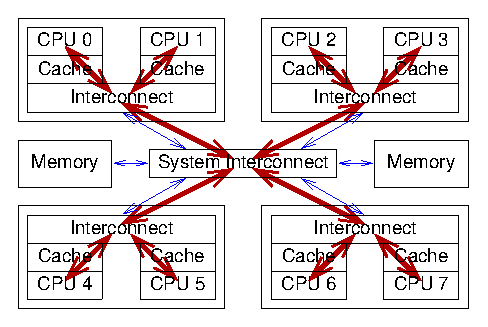
\includegraphics{count/GlobalTreeInc}}
\end{center}
\caption{Data Flow For Global Combining-Tree Atomic Increment}
\label{fig:count:Data Flow For Global Combining-Tree Atomic Increment}
\end{figure}

	If either or both of the first two conditions hold, there is
	\emph{some} hope for improved hardware.
	One could imagine the hardware implementing a combining tree,
	so that the increment requests from multiple CPUs are combined
	by the hardware into a single addition when the combined request
	reaches the hardware.
	The hardware could also apply an order to the requests, thus
	returning to each CPU the return value corresponding to its
	particular atomic increment.
	This results in instruction latency that varies as $O(log N)$,
	where $N$ is the number of CPUs, as shown in
	Figure~\ref{fig:count:Data Flow For Global Combining-Tree Atomic Increment}.
	And CPUs with this sort of hardware optimization are starting to
	appear as of 2011.

	This is a great improvement over the $O(N)$ performance
	of current hardware shown in
	Figure~\ref{fig:count:Data Flow For Global Atomic Increment},
	and it is possible that hardware latencies might decrease
	further if innovations such as three-dimensional fabrication prove
	practical.
	Nevertheless, we will see that in some important special cases,
	software can do \emph{much} better.

\QuickQ{}
	But doesn't the fact that C's ``integers'' are limited in size
	complicate things?
\QuickA{}
	No, because modulo addition is still commutative and associative.
	At least as long as you use unsigned integers.
	Recall that in the C standard, overflow of signed integers results
	in undefined behavior, never mind the fact that machines that
	do anything other than wrap on overflow are quite rare these days.
	Unfortunately, compilers frequently carry out optimizations that
	assume that signed integers will not overflow, so if your code
	allows signed integers to overflow, you can run into trouble
	even on twos-complement hardware.

	That said, one potential source of additional complexity arises
	when attempting to gather (say) a 64-bit sum from 32-bit
	per-thread counters.
	Dealing with this added complexity is left as
	an exercise for the reader, for whom some of the techniques
	introduced later in this chapter could be quite helpful.

\QuickQ{}
	An array???
	But doesn't that limit the number of threads?
\QuickA{}
	It can, and in this toy implementation, it does.
	But it is not that hard to come up with an alternative
	implementation that permits an arbitrary number of threads,
	for example, using the \co{gcc} \co{__thread} facility,
	as shown in
	Section~\ref{sec:count:Per-Thread-Variable-Based Implementation}.

\QuickQ{}
	What other choice does gcc have, anyway???
\QuickA{}
	According to the C standard, the effects of fetching a variable
	that might be concurrently modified by some other thread are
	undefined.
	It turns out that the C standard really has no other choice,
	given that C must support (for example) eight-bit architectures
	which are incapable of atomically loading a \co{long}.
	An upcoming version of the C standard aims to fill this gap,
	but until then, we depend on the kindness of the gcc developers.

	Alternatively, use of volatile accesses such as those provided
	by \co{ACCESS_ONCE()}~\cite{JonCorbet2012ACCESS:ONCE}
	can help constrain the compiler, at least
	in cases where the hardware is capable of accessing the value
	with a single memory-reference instruction.

\QuickQ{}
	How does the per-thread \co{counter} variable in
	Figure~\ref{fig:count:Array-Based Per-Thread Statistical Counters}
	get initialized?
\QuickA{}
	The C standard specifies that the initial value of
	global variables is zero, unless they are explicitly initialized.
	So the initial value of all the instances of \co{counter}
	will be zero.
	Furthermore, in the common case where the user is interested only
	in differences between consecutive reads
	from statistical counters, the initial value is irrelevant.

\QuickQ{}
	How is the code in
	Figure~\ref{fig:count:Array-Based Per-Thread Statistical Counters}
	supposed to permit more than one counter?
\QuickA{}
	Indeed, this toy example does not support more than one counter.
	Modifying it so that it can provide multiple counters is left
	as an exercise to the reader.

\QuickQ{}
	The read operation takes time to sum up the per-thread values,
	and during that time, the counter could well be changing.
	This means that the value returned by
	\co{read_count()} in
	Figure~\ref{fig:count:Array-Based Per-Thread Statistical Counters}
	will not necessarily be exact.
	Assume that the counter is being incremented at rate
	$r$ counts per unit time, and that \co{read_count()}'s
	execution consumes $\Delta$ units of time.
	What is the expected error in the return value?
\QuickA{}
	Let's do worst-case analysis first, followed by a less
	conservative analysis.

	In the worst case, the read operation completes immediately,
	but is then delayed for $\Delta$ time units before returning,
	in which case the worst-case error is simply $r \Delta$.

	This worst-case behavior is rather unlikely, so let us instead
	consider the case where the reads from each of the $N$
	counters is spaced equally over the time period $\Delta$.
	There will be $N+1$ intervals of duration $\frac{\Delta}{N+1}$
	between the $N$ reads.
	The error due to the delay after the read from the last thread's
	counter will be given by $\frac{r \Delta}{N \left( N + 1 \right)}$,
	the second-to-last thread's counter by
	$\frac{2 r \Delta}{N \left( N + 1 \right)}$,
	the third-to-last by
	$\frac{3 r \Delta}{N \left( N + 1 \right)}$,
	and so on.
	The total error is given by the sum of the errors due to the
	reads from each thread's counter, which is:

	\begin{equation}
		\frac{r \Delta}{N \left( N + 1 \right)}
			\sum_{i = 1}^N i
	\end{equation}

	Expressing the summation in closed form yields:

	\begin{equation}
		\frac{r \Delta}{N \left( N + 1 \right)}
			\frac{N \left( N + 1 \right)}{2}
	\end{equation}

	Cancelling yields the intuitively expected result:

	\begin{equation}
		\frac{r \Delta}{2}
	\label{eq:count:CounterErrorAverage}
	\end{equation}

	It is important to remember that error continues accumulating
	as the caller executes code making use of the count returned
	by the read operation.
	For example, if the caller spends time $t$ executing some
	computation based on the result of the returned count, the
	worst-case error will have increased to $r \left(\Delta + t\right)$.

	The expected error will have similarly increased to:

	\begin{equation}
		r \left( \frac{\Delta}{2} + t \right)
	\end{equation}

	Of course, it is sometimes unacceptable for the counter to
	continue incrementing during the read operation.
	Section~\ref{sec:count:Applying Specialized Parallel Counters}
	discusses a way to handle this situation.

	Thus far, we have been considering a counter that is only
	increased, never decreased.
	If the counter value is being changed by $r$ counts per unit
	time, but in either direction, we should expect the error
	to reduce.
	However, the worst case is unchanged because although the
	counter \emph{could} move in either direction, the worst
	case is whenthe read operation completes immediately,
	but then is delayed for $\Delta$ time units, during which
	time all the changes in the counter's value move it in
	the same direction, again giving us an absolute error
	of $r \Delta$.

	There are a number of ways to compute the average error,
	based on a variety of assumptions about the patterns of
	increments and decrements.
	For simplicity, let's assume that the $f$ fraction of
	the operations are decrements, and that the error of interest
	is the deviation from the counter's long-term trend line.
	Under this assumption, if $f$ is less than or equal to 0.5,
	each decrement will be cancelled by an increment, so that
	$2f$ of the operations will cancel each other, leaving
	$1-2f$ of the operations being uncancelled increments.
	On the other hand, if $f$ is greater than 0.5, $1-f$ of
	the decrements are cancelled by increments, so that the
	counter moves in the negative direction by $-1+2\left(1-f\right)$,
	which simplifies to $1-2f$, so that the counter moves an average
	of $1-2f$ per operation in either case.
	Therefore, that the long-term
	movement of the counter is given by $\left( 1-2f \right) r$.
	Plugging this into
	Equation~\ref{eq:count:CounterErrorAverage} yields:

	\begin{equation}
		\frac{\left( 1 - 2 f \right) r \Delta}{2}
	\end{equation}

	All that aside, in most uses of statistical counters, the
	error in the value returned by \co{read_count()} is
	irrelevant.
	This irrelevance is due to the fact that the time required
	for \co{read_count()} to execute is normally extremely
	small compared to the time interval between successive
	calls to \co{read_count()}.

\QuickQ{}
	Why doesn't \co{inc_count()} in
	Figure~\ref{fig:count:Array-Based Per-Thread Eventually Consistent Counters}
	need to use atomic instructions?
	After all, we now have multiple threads accessing the per-thread
	counters!
\QuickA{}
	Because one of the two threads only reads, and because the
	variable is aligned and machine-sized, non-atomic instructions
	suffice.
	That said, the \co{ACCESS_ONCE()} macro is used to prevent
	compiler optimizations that might otherwise prevent the
	counter updates from becoming visible to
	\co{eventual()}~\cite{JonCorbet2012ACCESS:ONCE}.

	An older version of this algorithm did in fact use atomic
	instructions, kudos to Ersoy Bayramoglu for pointing out that
	they are in fact unnecessary.
	That said, atomic instructions would be needed in cases where
	the per-thread \co{counter} variables were smaller than the
	global \co{global_count}.
	However, note that on a 32-bit system,
	the per-thread \co{counter} variables
	might need to be limited to 32 bits in order to sum them accurately,
	but with a 64-bit \co{global_count} variable to avoid overflow.
	In this case, it is necessary to zero the per-thead
	\co{counter} variables periodically in order to avoid overflow.
	It is extremely important to note that this zeroing cannot
	be delayed too long or overflow of the smaller per-thread
	variables will result.
	This approach therefore imposes real-time requirements on the
	underlying system, and in turn must be used with extreme care.

	In contrast, if all variables are the same size, overflow
	of any variable is harmless because the eventual sum
	will be modulo the word size.

\QuickQ{}
	Won't the single global thread in the function \co{eventual()} of
	Figure~\ref{fig:count:Array-Based Per-Thread Eventually Consistent Counters}
	be just as severe a bottleneck as a global lock would be?
\QuickA{}
	In this case, no.
	What will happen instead is that as the number of threads increases,
	the estimate of the counter
	value returned by \co{read_count()} will become more inaccurate.

\QuickQ{}
	Won't the estimate returned by \co{read_count()} in
	Figure~\ref{fig:count:Array-Based Per-Thread Eventually Consistent Counters}
	become increasingly
	inaccurate as the number of threads rises?
\QuickA{}
	Yes.
	If this proves problematic, one fix is to provide multiple
	\co{eventual()} threads, each covering its own subset of
	the other threads.
	In more extreme cases, a tree-like hierarchy of
	\co{eventual()} threads might be required.

\QuickQ{}
	Given that in the eventually-consistent algorithm shown in
	Figure~\ref{fig:count:Array-Based Per-Thread Eventually Consistent Counters}
	both reads and updates have extremely low overhead
	and are extremely scalable, why would anyone bother with the
	implementation described in
	Section~\ref{sec:count:Array-Based Implementation},
	given its costly read-side code?
\QuickA{}
	The thread executing \co{eventual()} consumes CPU time.
	As more of these eventually-consistent counters are added,
	the resulting \co{eventual()} threads will eventually
	consume all available CPUs.
	This implementation therefore suffers a different sort of
	scalability limitation, with the scalability limit being in
	terms of the number of eventually consistent counters rather
	than in terms of the number of threads or CPUs.

\QuickQ{}
	Why do we need an explicit array to find the other threads'
	counters?
	Why doesn't gcc provide a \co{per_thread()} interface, similar
	to the Linux kernel's \co{per_cpu()} primitive, to allow
	threads to more easily access each others' per-thread variables?
\QuickA{}
	Why indeed?

	To be fair, gcc faces some challenges that the Linux kernel
	gets to ignore.
	When a user-level thread exits, its per-thread variables all
	disappear, which complicates the problem of per-thread-variable
	access, particularly before the advent of user-level RCU
	(see Section~\ref{sec:defer:Read-Copy Update (RCU)}).
	In contrast, in the Linux kernel, when a CPU goes offline,
	that CPU's per-CPU variables remain mapped and accessible.

	Similarly, when a new user-level thread is created, its
	per-thread variables suddenly come into existence.
	In contrast, in the Linux kernel, all per-CPU variables are
	mapped and initialized at boot time, regardless of whether
	the corresponding CPU exists yet, or indeed, whether the
	corresponding CPU will ever exist.

	A key limitation that the Linux kernel imposes is a compile-time
	maximum bound on the number of CPUs, namely, \co{CONFIG_NR_CPUS},
	along with a typically tighter boot-time bound of \co{nr_cpu_ids}.
	In contrast, in user space, there is no hard-coded upper limit
	on the number of threads.

	Of course, both environments must handle dynamically loaded
	code (dynamic libraries in user space, kernel modules in the
	Linux kernel), which increases the complexity of per-thread
	variables.

	These complications make it significantly harder for user-space
	environments to provide access to other threads' per-thread
	variables.
	Nevertheless, such access is highly useful, and it is hoped
	that it will someday appear.

\QuickQ{}
	Doesn't the check for \co{NULL} on line~19 of
	Figure~\ref{fig:count:Per-Thread Statistical Counters}
	add extra branch mispredictions?
	Why not have a variable set permanently to zero, and point
	unused counter-pointers to that variable rather than setting
	them to \co{NULL}?
\QuickA{}
	This is a reasonable strategy.
	Checking for the performance difference is left as an exercise
	for the reader.
	However, please keep in mind that the fastpath is not
	\co{read_count()}, but rather \co{inc_count()}.

\QuickQ{}
	Why on earth do we need something as heavyweight as a \emph{lock}
	guarding the summation in the function \co{read_count()} in
	Figure~\ref{fig:count:Per-Thread Statistical Counters}?
\QuickA{}
	Remember, when a thread exits, its per-thread variables disappear.
	Therefore, if we attempt to access a given thread's per-thread
	variables after that thread exits, we will get a segmentation
	fault.
	The lock coordinates summation and thread exit, preventing this
	scenario.

	Of course, we could instead read-acquire a reader-writer lock,
	but Chapter~\ref{chp:Deferred Processing} will introduce even
	lighter-weight mechanisms for implementing the required coordination.

	Another approach would be to use an array instead of a per-thread
	variable, which, as Alexey Roytman notes, would eliminate
	the tests against \co{NULL}.
	However, array accesses are often slower than accesses to
	per-thread variables, and use of an array would imply a
	fixed upper bound on the number of threads.
	Also, note that neither tests nor locks are needed on the
	\co{inc_count()} fastpath.

\QuickQ{}
	Why on earth do we need to acquire the lock in
	\co{count_register_thread()} in
	Figure~\ref{fig:count:Per-Thread Statistical Counters}?
	It is a single properly aligned machine-word store to a location
	that no other thread is modifying, so it should be atomic anyway,
	right?
\QuickA{}
	This lock could in fact be omitted, but better safe than
	sorry, especially given that this function is executed only at
	thread startup, and is therefore not on any critical path.
	Now, if we were testing on machines with thousands of CPUs,
	we might need to omit the lock, but on machines with ``only''
	a hundred or so CPUs, there is no need to get fancy.

\QuickQ{}
	Fine, but the Linux kernel doesn't have to acquire a lock
	when reading out the aggregate value of per-CPU counters.
	So why should user-space code need to do this???
\QuickA{}
	Remember, the Linux kernel's per-CPU variables are always
	accessible, even if the corresponding CPU is offline --- even
	if the corresponding CPU never existed and never will exist.

\begin{figure}[tbp]
{ \scriptsize
\begin{verbatim}
  1 long __thread counter = 0;
  2 long *counterp[NR_THREADS] = { NULL };
  3 int finalthreadcount = 0;
  4 DEFINE_SPINLOCK(final_mutex);
  5 
  6 void inc_count(void)
  7 {
  8   counter++;
  9 }
 10 
 11 long read_count(void)
 12 {
 13   int t;
 14   long sum = 0;
 15 
 16   for_each_thread(t)
 17     if (counterp[t] != NULL)
 18       sum += *counterp[t];
 19   return sum;
 20 }
 21 
 22 void count_init(void)
 23 {
 24 }
 25 
 26 void count_register_thread(void)
 27 {
 28   counterp[smp_thread_id()] = &counter;
 29 }
 30 
 31 void count_unregister_thread(int nthreadsexpected)
 32 {
 33   spin_lock(&final_mutex);
 34   finalthreadcount++;
 35   spin_unlock(&final_mutex);
 36   while (finalthreadcount < nthreadsexpected)
 37     poll(NULL, 0, 1);
 38 }
\end{verbatim}
}
\caption{Per-Thread Statistical Counters With Lockless Summation}
\label{fig:count:Per-Thread Statistical Counters With Lockless Summation}
\end{figure}

	One workaround is to ensure that each thread continues to exist
	until all threads are finished, as shown in
	Figure~\ref{fig:count:Per-Thread Statistical Counters With Lockless Summation}
	(\co{count_tstat.c}).
	Analysis of this code is left as an exercise to the reader,
	however, please note that it does not fit well into the
	\url{counttorture.h} counter-evaluation scheme.
	(Why not?)
	Chapter~\ref{chp:Deferred Processing} will introduce 
	synchronization mechanisms that handle this situation in a much
	more graceful manner.

\QuickQ{}
	What fundamental difference is there between counting packets
	and counting the total number of bytes in the packets, given
	that the packets vary in size?
\QuickA{}
	When counting packets, the counter is only incremented by the
	value one.
	On the other hand, when counting bytes, the counter might
	be incremented by largish numbers.

	Why does this matter?
	Because in the increment-by-one case, the value returned will
	be exact in the sense that the counter must necessarily have
	taken on that value at some point in time, even if it is impossible
	to say precisely when that point occurred.
	In contrast, when counting bytes, two different threads might
	return values that are inconsistent with any global ordering
	of operations.

	To see this, suppose that thread~0 adds the value three to its
	counter, thread~1 adds the value five to its counter, and
	threads~2 and 3 sum the counters.
	If the system is ``weakly ordered'' or if the compiler
	uses aggressive optimizations, thread~2 might find the
	sum to be three and thread~3 might find the sum to be five.
	The only possible global orders of the sequence of values
	of the counter are 0,3,8 and 0,5,8, and neither order is
	consistent with the results obtained.

	If you missed this one, you are not alone.
	Michael Scott used this question to stump Paul E.~McKenney
	during Paul's Ph.D. defense.

\QuickQ{}
	Given that the reader must sum all the threads' counters,
	this could take a long time given large numbers of threads.
	Is there any way that the increment operation can remain
	fast and scalable while allowing readers to also enjoy
	reasonable performance and scalability?
\QuickA{}
	One approach would be to maintain a global approximation
	to the value.
	Readers would increment their per-thread variable, but when it
	reached some predefined limit, atomically add it to a global
	variable, then zero their per-thread variable.
	This would permit a tradeoff between average increment overhead
	and accuracy of the value read out.

	The reader is encouraged to think up and try out other approaches,
	for example, using a combining tree.

\QuickQ{}
	Why does
	Figure~\ref{fig:count:Simple Limit Counter Add, Subtract, and Read}
	provide \co{add_count()} and \co{sub_count()} instead of the
	\co{inc_count()} and \co{dec_count()} interfaces show in
	Section~\ref{sec:count:Statistical Counters}?
\QuickA{}
	Because structures come in different sizes.
	Of course, a limit counter corresponding to a specific size
	of structure might still be able to use
	\co{inc_count()} and \co{dec_count()}.

\QuickQ{}
	What is with the strange form of the condition on line~3 of
	Figure~\ref{fig:count:Simple Limit Counter Add, Subtract, and Read}?
	Why not the following more intuitive form of the fastpath?

	\vspace{5pt}
	\begin{minipage}[t]{\columnwidth}
	\small
	\begin{verbatim}
  3 if (counter + delta <= countermax){
  4   counter += delta;
  5   return 1;
  6 }
	\end{verbatim}
	\end{minipage}
	\vspace{5pt}
\QuickA{}
	Two words.
	``Integer overflow.''

	Try the above formulation with \co{counter} equal to 10 and
	\co{delta} equal to \co{ULONG_MAX}.
	Then try it again with the code shown in
	Figure~\ref{fig:count:Simple Limit Counter Add, Subtract, and Read}.

	A good understanding of integer overflow will be required for
	the rest of this example, so if you have never dealt with
	integer overflow before, please try several examples to get
	the hang of it.
	Integer overflow can sometimes be more difficult to get right
	than parallel algorithms!

\QuickQ{}
	Why does \co{globalize_count()} zero the per-thread variables,
	only to later call \co{balance_count()} to refill them in
	Figure~\ref{fig:count:Simple Limit Counter Add, Subtract, and Read}?
	Why not just leave the per-thread variables non-zero?
\QuickA{}
	That is in fact what an earlier version of this code did.
	But addition and subtraction are extremely cheap, and handling
	all of the special cases that arise is quite complex.
	Again, feel free to try it yourself, but beware of integer
	overflow!

\QuickQ{}
	Given that \co{globalreserve} counted against us in \co{add_count()},
	why doesn't it count for us in \co{sub_count()} in
	Figure~\ref{fig:count:Simple Limit Counter Add, Subtract, and Read}?
\QuickA{}
	The \co{globalreserve} variable tracks the sum of all threads'
	\co{countermax} variables.
	The sum of these threads' \co{counter} variables might be anywhere
	from zero to \co{globalreserve}.
	We must therefore take a conservative approach, assuming that
	all threads' \co{counter} variables are full in \co{add_count()}
	and that they are all empty in \co{sub_count()}.

	But remember this question, as we will come back to it later.

\QuickQ{}
	Suppose that one thread invokes \co{add_count()} shown in
	Figure~\ref{fig:count:Simple Limit Counter Add, Subtract, and Read},
	and then another thread invokes \co{sub_count()}.
	Won't \co{sub_count()} return failure even though the value of
	the counter is non-zero?
\QuickA{}
	Indeed it will!
	In many cases, this will be a problem, as discussed in
	Section~\ref{sec:count:Simple Limit Counter Discussion}, and
	in those cases the algorithms from
	Section~\ref{sec:count:Exact Limit Counters}
	will likely be preferable.

\QuickQ{}
	Why have both \co{add_count()} and \co{sub_count()} in
	Figure~\ref{fig:count:Simple Limit Counter Add, Subtract, and Read}?
	Why not simply pass a negative number to \co{add_count()}?
\QuickA{}
	Given that \co{add_count()} takes an \co{unsigned} \co{long}
	as its argument, it is going to be a bit tough to pass it a
	negative number.
	And unless you have some anti-matter memory, there is little
	point in allowing negative numbers when counting the number
	of structures in use!

\QuickQ{}
	Why set \co{counter} to \co{countermax / 2} in line~15 of
	Figure~\ref{fig:count:Simple Limit Counter Utility Functions}?
	Wouldn't it be simpler to just take \co{countermax} counts?
\QuickA{}
	First, it really is reserving \co{countermax} counts
	(see line~14), however,
	it adjusts so that only half of these are actually in use
	by the thread at the moment.
	This allows the thread to carry out at least \co{countermax / 2}
	increments or decrements before having to refer back to
	\co{globalcount} again.

	Note that the accounting in \co{globalcount} remains accurate,
	thanks to the adjustment in line~18.

\QuickQ{}
	In Figure~\ref{fig:count:Schematic of Globalization and Balancing},
	even though a quarter of the remaining count up to the limit is
	assigned to thread~0, only an eighth of the remaining count is
	consumed, as indicated by the uppermost dotted line connecting
	the center and the rightmost configurations.
	Why is that?
\QuickA{}
	The reason this happened is that thread~0's \co{counter} was
	set to half of its \co{countermax}.
	Thus, of the quarter assigned to thread~0, half of that quarter
	(one eighth) came from \co{globalcount}, leaving the other half
	(again, one eighth) to come from the remaining count.

	There are two purposes for taking this approach:
	(1)~To allow thread~0 to use the fastpath for decrements as
	well as increments, and
	(2)~To reduce the inaccuracies if all threads are monotonically
	incrementing up towards the limit.
	To see this last point, step through the algorithm and watch
	what it does.

\QuickQ{}
	Why is it necessary to atomically manipulate the thread's
	\co{counter} and \co{countermax} variables as a unit?
	Wouldn't it be good enough to atomically manipulate them
	individually?
\QuickA{}
	This might well be possible, but great care is required.
	Note that removing \co{counter} without first zeroing
	\co{countermax} could result in the corresponding thread
	increasing \co{counter} immediately after it was zeroed,
	completely negating the effect of zeroing the counter.

	The opposite ordering, namely zeroing \co{countermax} and then
	removing \co{counter}, can also result in a non-zero
	\co{counter}.
	To see this, consider the following sequence of events:

	\begin{enumerate}
	\item	Thread~A fetches its \co{countermax}, and finds that
		it is non-zero.
	\item	Thread~B zeroes Thread~A's \co{countermax}.
	\item	Thread~B removes Thread~A's \co{counter}.
	\item	Thread~A, having found that its \co{countermax}
		is non-zero, proceeds to add to its \co{counter},
		resulting in a non-zero value for \co{counter}.
	\end{enumerate}

	Again, it might well be possible to atomically manipulate
	\co{countermax} and \co{counter} as separate variables,
	but it is clear that great care is required.
	It is also quite likely that doing so will slow down the
	fastpath.

	Exploring these possibilities are left as exercises for
	the reader.

\QuickQ{}
	In what way does line~7 of
	Figure~\ref{fig:count:Atomic Limit Counter Variables and Access Functions}
	violate the C standard?
\QuickA{}
	It assumes eight bits per byte.
	This assumption does hold for all current commodity microprocessors
	that can be easily assembled into shared-memory multiprocessors,
	but certainly does not hold for all computer systems that have
	ever run C code.
	(What could you do instead in order to comply with the C
	standard?  What drawbacks would it have?)

\QuickQ{}
	Given that there is only one \co{ctrandmax} variable,
	why bother passing in a pointer to it on line~18 of
	Figure~\ref{fig:count:Atomic Limit Counter Variables and Access Functions}?
\QuickA{}
	There is only one \co{ctrandmax} variable \emph{per thread}.
	Later, we will see code that needs to pass other threads'
	\co{ctrandmax} variables to \co{split_ctrandmax()}.

\QuickQ{}
	Why does \co{merge_ctrandmax()} in
	Figure~\ref{fig:count:Atomic Limit Counter Variables and Access Functions}
	return an \co{int} rather than storing directly into an
	\co{atomic_t}?
\QuickA{}
	Later, we will see that we need the \co{int} return to pass
	to the \co{atomic_cmpxchg()} primitive.

\QuickQ{}
	Yecch!
	Why the ugly \co{goto} on line~11 of
	Figure~\ref{fig:count:Atomic Limit Counter Add and Subtract}?
	Haven't you heard of the \co{break} statement???
\QuickA{}
	Replacing the \co{goto} with a \co{break} would require keeping
	a flag to determine whether or not line~15 should return, which
	is not the sort of thing you want on a fastpath.
	If you really hate the \co{goto} that much, your best bet would
	be to pull the fastpath into a separate function that returned
	success or failure, with ``failure'' indicating a need for the
	slowpath.
	This is left as an exercise for goto-hating readers.

\QuickQ{}
	Why would the \co{atomic_cmpxchg()} primitive at lines~13-14 of
	Figure~\ref{fig:count:Atomic Limit Counter Add and Subtract}
	ever fail?
	After all, we picked up its old value on line~9 and have not
	changed it!
\QuickA{}
	Later, we will see how the \co{flush_local_count()} function in
	Figure~\ref{fig:count:Atomic Limit Counter Utility Functions 1}
	might update this thread's \co{ctrandmax} variable concurrently
	with the execution of the fastpath on lines~8-14 of
	Figure~\ref{fig:count:Atomic Limit Counter Add and Subtract}.

\QuickQ{}
	What stops a thread from simply refilling its
	\co{ctrandmax} variable immediately after
	\co{flush_local_count()} on line 14 of
	Figure~\ref{fig:count:Atomic Limit Counter Utility Functions 1}
	empties it?
\QuickA{}
	This other thread cannot refill its \co{ctrandmax}
	until the caller of \co{flush_local_count()} releases the
	\co{gblcnt_mutex}.
	By that time, the caller of \co{flush_local_count()} will have
	finished making use of the counts, so there will be no problem
	with this other thread refilling --- assuming that the value
	of \co{globalcount} is large enough to permit a refill.

\QuickQ{}
	What prevents concurrent execution of the fastpath of either
	\co{add_count()} or \co{sub_count()} from interfering with
	the \co{ctrandmax} variable while
	\co{flush_local_count()} is accessing it on line 27 of
	Figure~\ref{fig:count:Atomic Limit Counter Utility Functions 1}
	empties it?
\QuickA{}
	Nothing.
	Consider the following three cases:
	\begin{enumerate}
	\item	If \co{flush_local_count()}'s \co{atomic_xchg()} executes
		before the \co{split_ctrandmax()} of either fastpath,
		then the fastpath will see a zero \co{counter} and
		\co{countermax}, and will thus transfer to the slowpath
		(unless of course \co{delta} is zero).
	\item	If \co{flush_local_count()}'s \co{atomic_xchg()} executes
		after the \co{split_ctrandmax()} of either fastpath,
		but before that fastpath's \co{atomic_cmpxchg()},
		then the \co{atomic_cmpxchg()} will fail, causing the
		fastpath to restart, which reduces to case~1 above.
	\item	If \co{flush_local_count()}'s \co{atomic_xchg()} executes
		after the \co{atomic_cmpxchg()} of either fastpath,
		then the fastpath will (most likely) complete successfully
		before \co{flush_local_count()} zeroes the thread's
		\co{ctrandmax} variable.
	\end{enumerate}
	Either way, the race is resolved correctly.

\QuickQ{}
	Given that the \co{atomic_set()} primitive does a simple
	store to the specified \co{atomic_t}, how can line~21 of
	\co{balance_count()} in
	Figure~\ref{fig:count:Atomic Limit Counter Utility Functions 2}
	work correctly in face of concurrent \co{flush_local_count()}
	updates to this variable?
\QuickA{}
	The caller of both \co{balance_count()} and
	\co{flush_local_count()} hold \co{gblcnt_mutex}, so
	only one may be executing at a given time.

\QuickQ{}
	But signal handlers can be migrated to some other
	CPU while running.
	Doesn't this possibility require that atomic instructions
	and memory barriers are required to reliably communicate
	between a thread and a signal handler that interrupts that
	thread?
\QuickA{}
	No.
	If the signal handler is migrated to another CPU, then the
	interrupted thread is also migrated along with it.

\QuickQ{}
	In Figure~\ref{fig:count:Signal-Theft State Machine}, why is
	the REQ \co{theft} state colored red?
\QuickA{}
	To indicate that only the fastpath is permitted to change the
	\co{theft} state, and that if the thread remains in this
	state for too long, the thread running the slowpath will
	resend the POSIX signal.

\QuickQ{}
	In Figure~\ref{fig:count:Signal-Theft State Machine}, what is
	the point of having separate REQ and ACK \co{theft} states?
	Why not simplify the state machine by collapsing
	them into a single REQACK state?
	Then whichever of the signal handler or the fastpath gets there
	first could set the state to READY.
\QuickA{}
	Reasons why collapsing the REQ and ACK states would be a very
	bad idea include:
	\begin{enumerate}
	\item	The slowpath uses the REQ and ACK states to determine
		whether the signal should be retransmitted.
		If the states were collapsed, the slowpath would have
		no choice but to send redundant signals, which would
		have the unhelpful effect of needlessly slowing down
		the fastpath.
	\item	The following race would result:
		\begin{enumerate}
		\item	The slowpath sets a given thread's state to REQACK.
		\item	That thread has just finished its fastpath, and
			notes the REQACK state.
		\item	The thread receives the signal, which also notes
			the REQACK state, and, because there is no fastpath
			in effect, sets the state to READY.
		\item	The slowpath notes the READY state, steals the
			count, and sets the state to IDLE, and completes.
		\item	The fastpath sets the state to READY, disabling
			further fastpath execution for this thread.
		\end{enumerate}
		The basic problem here is that the combined REQACK state
		can be referenced by both the signal handler and the
		fastpath.
		The clear separation maintained by the four-state
		setup ensures orderly state transitions.
	\end{enumerate}
	That said, you might well be able to make a three-state setup
	work correctly.
	If you do succeed, compare carefully to the four-state setup.
	Is the three-state solution really preferable, and why or why not?

\QuickQ{}
	In Figure~\ref{fig:count:Signal-Theft Limit Counter Value-Migration Functions}
	function \co{flush_local_count_sig()}, why are there
	\co{ACCESS_ONCE()} wrappers around the uses of the
	\co{theft} per-thread variable?
\QuickA{}
	The first one (on line~11) can be argued to be unnecessary.
	The last two (lines~14 and 16) are important.
	If these are removed, the compiler would be within its rights
	to rewrite lines~14-17 as follows:
	\vspace{5pt}
	\begin{minipage}[t]{\columnwidth}
	\small
	\begin{verbatim}
 14   theft = THEFT_READY;
 15   if (counting) {
 16     theft = THEFT_ACK;
 17   }
	\end{verbatim}
	\end{minipage}
	\vspace{5pt}
	This would be fatal, as the slowpath might see the transient
	value of \co{THEFT_READY}, and start stealing before the
	corresponding thread was ready.

\QuickQ{}
	In Figure~\ref{fig:count:Signal-Theft Limit Counter Value-Migration Functions},
	why is it safe for line~28 to directly access the other thread's
	\co{countermax} variable?
\QuickA{}
	Because the other thread is not permitted to change the value
	of its \co{countermax} variable unless it holds the
	\co{gblcnt_mutex} lock.
	But the caller has acquired this lock, so it is not possible
	for the other thread to hold it, and therefore the other thread
	is not permitted to change its \co{countermax} variable.
	We can therefore safely access it --- but not change it.

\QuickQ{}
	In Figure~\ref{fig:count:Signal-Theft Limit Counter Value-Migration Functions},
	why doesn't line~33 check for the current thread sending itself
	a signal?
\QuickA{}
	There is no need for an additional check.
	The caller of \co{flush_local_count()} has already invoked
	\co{globalize_count()}, so the check on line~28 will have
	succeeded, skipping the later \co{pthread_kill()}.

\QuickQ{}
	The code in
	Figure~\ref{fig:count:Signal-Theft Limit Counter Value-Migration Functions},
	works with gcc and POSIX.
	What would be required to make it also conform to the ISO C standard?
\QuickA{}
	The \co{theft} variable must be of type \co{sig_atomic_t}
	to guarantee that it can be safely shared between the signal
	handler and the code interrupted by the signal.

\QuickQ{}
	In Figure~\ref{fig:count:Signal-Theft Limit Counter Value-Migration Functions}, why does line~41 resend the signal?
\QuickA{}
	Because many operating systems over several decades have
	had the property of losing the occasional signal.
	Whether this is a feature or a bug is debatable, but
	irrelevant.
	The obvious symptom from the user's viewpoint will not be
	a kernel bug, but rather a user application hanging.

	\emph{Your} user application hanging!

\QuickQ{}
	Not only are POSIX signals slow, sending one to each thread
	simply does not scale.
	What would you do if you had (say) 10,000 threads and needed
	the read side to be fast?
\QuickA{}
	One approach is to use the techniques shown in
	Section~\ref{sec:count:Eventually Consistent Implementation},
	summarizing an approximation to the overall counter value in
	a single variable.
	Another approach would be to use multiple threads to carry
	out the reads, with each such thread interacting with a
	specific subset of the updating threads.

\QuickQ{}
	What if you want an exact limit counter to be exact only for
	its lower limit, but to allow the upper limit to be inexact?
\QuickA{}
	One simple solution is to overstate the upper limit by the
	desired amount.
	The limiting case of such overstatement results in the
	upper limit being set to the largest value that the counter is
	capable of representing.

\QuickQ{}
	What else had you better have done when using a biased counter?
\QuickA{}
	You had better have set the upper limit to be large enough
	accommodate the bias, the expected maximum number of accesses,
	and enough ``slop'' to allow the counter to work efficiently
	even when the number of accesses is at its maximum.

\QuickQ{}
	This is ridiculous!
	We are \emph{read}-acquiring a reader-writer lock to
	\emph{update} the counter?
	What are you playing at???
\QuickA{}
	Strange, perhaps, but true!
	Almost enough to make you think that the name
	``reader-writer lock'' was poorly chosen, isn't it?

\QuickQ{}
	What other issues would need to be accounted for in a real system?
\QuickA{}
	A huge number!

	Here are a few to start with:

	\begin{enumerate}
	\item	There could be any number of devices, so that the
		global variables are inappropriate, as are the
		lack of arguments to functions like \co{do_io()}.
	\item	Polling loops can be problematic in real systems.
		In many cases, it is far better to have the last
		completing I/O wake up the device-removal thread.
	\item	The I/O might fail, and so \co{do_io()} will likely
		need a return value.
	\item	If the device fails, the last I/O might never complete.
		In such cases, there might need to be some sort of
		timeout to allow error recovery.
	\item	Both \co{add_count()} and \co{sub_count()} can
		fail, but their return values are not checked.
	\item	Reader-writer locks do not scale well.
		One way of avoiding the high read-acquisition costs
		of reader-writer locks is presented in
		Chapters~\ref{chp:Locking}
		and~\ref{chp:Deferred Processing}.
	\item	The polling loops result in poor energy efficiency.
		An event-driven design is preferable.
	\end{enumerate}

\QuickQ{}
	On the \url{count_stat.c} row of
	Table~\ref{tab:count:Statistical Counter Performance on Power-6},
	we see that the update side scales linearly with the number of
	threads.
	How is that possible given that the more threads there are,
	the more per-thread counters must be summed up?
\QuickA{}
	The read-side code must scan the entire fixed-size array, regardless
	of the number of threads, so there is no difference in performance.
	In contrast, in the last two algorithms, readers must do more
	work when there are more threads.
	In addition, the last two algorithms interpose an additional
	level of indirection because they map from integer thread ID
	to the corresponding \co{__thread} variable.

\QuickQ{}
	Even on the last row of
	Table~\ref{tab:count:Statistical Counter Performance on Power-6},
	the read-side performance of these statistical counter
	implementations is pretty horrible.
	So why bother with them?
\QuickA{}
	``Use the right tool for the job.''

	As can be seen from
	Figure~\ref{fig:count:Atomic Increment Scalability on Nehalem},
	single-variable atomic increment need not apply for any job
	involving heavy use of parallel updates.
	In contrast, the algorithms shown in
	Table~\ref{tab:count:Statistical Counter Performance on Power-6}
	do an excellent job of handling update-heavy situations.
	Of course, if you have a read-mostly situation, you should
	use something else, for example, an eventually consistent design
	featuring a single atomically incremented
	variable that can be read out using a single load,
	similar to the approach used in
	Section~\ref{sec:count:Eventually Consistent Implementation}.

\QuickQ{}
	Given the performance data shown in
	Table~\ref{tab:count:Limit Counter Performance on Power-6},
	we should always prefer signals over atomic operations, right?
\QuickA{}
	That depends on the workload.
	Note that on a 64-core system, you need more than
	one hundred non-atomic operations (with roughly
	a 40-nanosecond performance gain) to make up for even one
	signal (with almost a 5-\emph{microsecond} performance loss).
	Although there are no shortage of workloads with far greater
	read intensity, you will need to consider your particular
	workload.

	In addition, although memory barriers have historically been
	expensive compared to ordinary instructions, you should
	check this on the specific hardware you will be running.
	The properties of computer hardware do change over time,
	and algorithms must change accordingly.

\QuickQ{}
	Can advanced techniques be applied to address the lock
	contention for readers seen in
	Table~\ref{tab:count:Limit Counter Performance on Power-6}?
\QuickA{}
	One approach is to give up some update-side performance, as is
	done with scalable non-zero indicators
	(SNZI)~\cite{FaithEllen:2007:SNZI}.
	There are a number of other ways one might go about this, and these
	are left as exercises for the reader.
	Any number of approaches that apply hierarchy, which replace
	frequent global-lock acquisitions with local lock acquisitions
	corresponding to lower levels of the hierarchy, should work quite well.

\QuickQ{}
	The \co{++} operator works just fine for 1,000-digit numbers!
	Haven't you heard of operator overloading???
\QuickA{}
	In the C++ language, you might well be able to use \co{++}
	on a 1,000-digit number, assuming that you had access to a
	class implementing such numbers.
	But as of 2010, the C language does not permit operator overloading.

\QuickQ{}
	But if we are going to have to partition everything, why bother
	with shared-memory multithreading?
	Why not just partition the problem completely and run as
	multiple processes, each in its own address space?
\QuickA{}
	Indeed, multiple processes with separate address spaces can be
	an excellent way to exploit parallelism, as the proponents of
	the fork-join methodology and the Erlang language would be very
	quick to tell you.
	However, there are also some advantages to shared-memory parallelism:
	\begin{enumerate}
	\item	Only the most performance-critical portions of the
		application must be partitioned, and such portions
		are usually a small fraction of the application.
	\item	Although cache misses are quite slow compared to
		individual register-to-register instructions,
		they are typically considerably faster than
		inter-process-communication primitives, which in
		turn are considerably faster than things like
		TCP/IP networking.
	\item	Shared-memory multiprocessors are readily available
		and quite inexpensive, so, in stark contrast to the
		1990s, there is little cost penalty for use of
		shared-memory parallelism.
	\end{enumerate}
	As always, use the right tool for the job!

\QuickQAC{cha:Partitioning and Synchronization Design}{Partitioning and Synchronization Design}
\QuickQ{}
	Is there a better solution to the Dining
	Philosophers Problem?
\QuickA{}

\begin{figure}[tb]
\begin{center}
\includegraphics[scale=.7]{SMPdesign/DiningPhilosopher5PEM}
\end{center}
\caption{Dining Philosophers Problem, Fully Partitioned}
\ContributedBy{Figure}{fig:SMPdesign:Dining Philosophers Problem, Fully Partitioned}{Kornilios Kourtis}
\end{figure}

	One such improved solution is shown in
	Figure~\ref{fig:SMPdesign:Dining Philosophers Problem, Fully Partitioned},
	where the philosophers are simply provided with an additional
	five forks.
	All five philosophers may now eat simultaneously, and there
	is never any need for philosophers to wait on one another.
	In addition, this approach offers greatly improved disease control.

	This solution might seem like cheating to some, but such
	``cheating'' is key to finding good solutions to many
	concurrency problems.

\QuickQ{}
	And in just what sense can this ``horizontal parallelism'' be
	said to be ``horizontal''?
\QuickA{}
	Inman was working with protocol stacks, which are normally
	depicted vertically, with the application on top and the
	hardware interconnect on the bottom.
	Data flows up and down this stack.
	``Horizontal parallelism'' processes packets from different network
	connections in parallel, while ``vertical parallelism''
	handles different protocol-processing steps for a given
	packet in parallel.

	``Vertical parallelism'' is also called ``pipelining''.

\QuickQ{}
	In this compound double-ended queue implementation, what should
	be done if the queue has become non-empty while releasing
	and reacquiring the lock?
\QuickA{}
	In this case, simply dequeue an item from the non-empty
	queue, release both locks, and return.

\QuickQ{}
	Is the hashed double-ended queue a good solution?
	Why or why not?
\QuickA{}
	The best way to answer this is to run \url{lockhdeq.c} on
	a number of different multiprocessor systems, and you are
	encouraged to do so in the strongest possible terms.
	One reason for concern is that each operation on this
	implementation must acquire not one but two locks.
	% Getting about 500 nanoseconds per element when used as
	% a queue on a 4.2GHz Power system.  This is roughly the same as
	% the version covered by a single lock.  Sequential (unlocked
	% variant is more than an order of magnitude faster!

	The first well-designed performance study will be cited.\footnote{
		The studies by Dalessandro
		et al.~\cite{LukeDalessandro:2011:ASPLOS:HybridNOrecSTM:deque}
		and Dice et al.~\cite{DavidDice:2010:SCA:HTM:deque} are
		good starting points.}
	Do not forget to compare to a sequential implementation!

\QuickQ{}
	Move \emph{all} the elements to the queue that became empty?
	In what possible universe is this brain-dead solution in any
	way optimal???
\QuickA{}
	It is optimal in the case where data flow switches direction only
	rarely.
	It would of course be an extremely poor choice if the double-ended
	queue was being emptied from both ends concurrently.
	This of course raises another question, namely, in what possible
	universe emptying from both ends concurrently would be a reasonable
	thing to do.
	Work-stealing queues are one possible answer to this question.

\QuickQ{}
	Why can't the compound parallel double-ended queue
	implementation be symmetric?
\QuickA{}
	The need to avoid deadlock by imposing a lock hierarchy
	forces the asymmetry, just as it does in the fork-numbering
	solution to the Dining Philosophers Problem
	(see Section~\ref{sec:SMPdesign:Dining Philosophers Problem}).

\QuickQ{}
	Why is it necessary to retry the right-dequeue operation
	on line~28 of
	Figure~\ref{fig:SMPdesign:Compound Parallel Double-Ended Queue Implementation}?
\QuickA{}
	This retry is necessary because some other thread might have
	enqueued an element between the time that this thread dropped
	\co{d->rlock} on line~25 and the time that it reacquired this
	same lock on line~27.

\QuickQ{}
	Surely the left-hand lock must \emph{sometimes} be available!!!
	So why is it necessary that line~25 of
	Figure~\ref{fig:SMPdesign:Compound Parallel Double-Ended Queue Implementation}
	unconditionally release the right-hand lock?
\QuickA{}
	It would be possible to use \co{spin_trylock()} to attempt
	to acquire the left-hand lock when it was available.
	However, the failure case would still need to drop the
	right-hand lock and then re-acquire the two locks in order.
	Making this transformation (and determining whether or not
	it is worthwhile) is left as an exercise for the reader.

\QuickQ{}
	Why are there not one but two solutions to the double-ended queue
	problem?
\QuickA{}
	There are actually at least three.
	The third, by Dominik Dingel, makes interesting use of
	reader-writer locking, and may be found in \co{lockrwdeq.c}.

\QuickQ{}
	The tandem double-ended queue runs about twice as fast as
	the hashed double-ended queue, even when I increase the
	size of the hash table to an insanely large number.
	Why is that?
\QuickA{}
	The hashed double-ended queue's locking design only permits
	one thread at a time at each end, and further requires
	two lock acquisitions for each operation.
	The tandem double-ended queue also permits one thread at a time
	at each end, and in the common case requires only one lock
	acquisition per operation.
	Therefore, the tandem double-ended queue should be expected to
	outperform the hashed double-ended queue.

	Can you created a double-ended queue that allows multiple
	concurrent operations at each end?
	If so, how?  If not, why not?

\QuickQ{}
	Is there a significantly better way of handling concurrency
	for double-ended queues?
\QuickA{}
	One approach is to transform the problem to be solved
	so that multiple double-ended queues can be used in parallel,
	allowing the simpler single-lock double-ended queue to be used,
	and perhaps also replace each double-ended queue with a pair of
	conventional single-ended queues.
	Without such ``horizontal scaling'', the speedup is limited
	to 2.0.
	In contrast, horizontal-scaling designs can achieve very large
	speedups, and are especially attractive if there are multiple threads
	working either end of the queue, because in this
	multiple-thread case the dequeue
	simply cannot provide strong ordering guarantees.
	After all, the fact that a given thread removed an item first
	in no way implies that it will process that item
	first~\cite{AndreasHaas2012FIFOisnt}.
	And if there are no guarantees, we may as well obtain the
	performance benefits that come with refusing to provide these
	guarantees.
	% about twice as fast as hashed version on 4.2GHz Power.

	Regardless of whether or not the problem can be transformed
	to use multiple queues, it is worth asking whether work can
	be batched so that each enqueue and dequeue operation corresponds
	to larger units of work.
	This batching approach decreases contention on the queue data
	structures, which increases both performance and scalability,
	as will be seen in
	Section~\ref{sec:SMPdesign:Synchronization Granularity}.
	After all, if you must incur high synchronization overheads,
	be sure you are getting your money's worth.

	Other researchers are working on other ways to take advantage
	of limited ordering guarantees in
	queues~\cite{ChristophMKirsch2012FIFOisntTR}.

\QuickQ{}
	Don't all these problems with critical sections mean that
	we should just always use
	non-blocking synchronization~\cite{MauriceHerlihy90a},
	which don't have critical sections?
\QuickA{}
	Although non-blocking synchronization can be very useful
	in some situations, it is no panacea.
	Also, non-blocking synchronization really does have
	critical sections, as noted by Josh Triplett.
	For example, in a non-blocking algorithm based on
	compare-and-swap operations, the code starting at the
	initial load and continuing to the compare-and-swap
	is in many ways analogous to a lock-based critical section.

\QuickQ{}
	What are some ways of preventing a structure from being freed while
	its lock is being acquired?
\QuickA{}
	Here are a few possible solutions to this \emph{existence guarantee}
	problem:

	\begin{enumerate}
	\item	Provide a statically allocated lock that is held while
		the per-structure lock is being acquired, which is an
		example of hierarchical locking (see
		Section~\ref{sec:SMPdesign:Hierarchical Locking}).
		Of course, using a single global lock for this purpose
		can result in unacceptably high levels of lock contention,
		dramatically reducing performance and scalability.
	\item	Provide an array of statically allocated locks, hashing
		the structure's address to select the lock to be acquired,
		as described in Chapter~\ref{chp:Locking}.
		Given a hash function of sufficiently high quality, this
		avoids the scalability limitations of the single global
		lock, but in read-mostly situations, the lock-acquisition
		overhead can result in unacceptably degraded performance.
	\item	Use a garbage collector, in software environments providing
		them, so that a structure cannot be deallocated while being
		referenced.
		This works very well, removing the existence-guarantee
		burden (and much else besides) from the developer's
		shoulders, but imposes the overhead of garbage collection
		on the program.
		Although garbage-collection technology has advanced
		considerably in the past few decades, its overhead
		may be unacceptably high for some applications.
		In addition, some applications require that the developer
		exercise more control over the layout and placement of
		data structures than is permitted by most garbage collected
		environments.
	\item	As a special case of a garbage collector, use a global
		reference counter, or a global array of reference counters.
	\item	Use \emph{hazard pointers}~\cite{MagedMichael04a}, which
		can be thought of as an inside-out reference count.
		Hazard-pointer-based algorithms maintain a per-thread list of
		pointers, so that the appearance of a given pointer on
		any of these lists acts as a reference to the corresponding
		structure.
		Hazard pointers are an interesting research direction, but
		have not yet seen much use in production (written in 2008).
	\item	Use transactional memory
		(TM)~\cite{Herlihy93a,DBLomet1977SIGSOFT,Shavit95},
		so that each reference and
		modification to the data structure in question is
		performed atomically.
		Although TM has engendered much excitement in recent years,
		and seems likely to be of some use in production software,
		developers should exercise some
		caution~\cite{Blundell2005DebunkTM,Blundell2006TMdeadlock,McKenney2007PLOSTM},
		particularly in performance-critical code.
		In particular, existence guarantees require that the
		transaction cover the full path from a global reference
		to the data elements being updated.
	\item	Use RCU, which can be thought of as an extremely lightweight
		approximation to a garbage collector.
		Updaters are not permitted to free RCU-protected
		data structures that RCU readers might still be referencing.
		RCU is most heavily used for read-mostly data structures,
		and is discussed at length in
		Chapter~\ref{chp:Deferred Processing}.
	\end{enumerate}

	For more on providing existence guarantees, see
	Chapters~\ref{chp:Locking} and \ref{chp:Deferred Processing}.

\QuickQ{}
	How can a single-threaded 64-by-64 matrix multiple possibly
	have an efficiency of less than 1.0?
	Shouldn't all of the traces in
	Figure~\ref{fig:SMPdesign:Matrix Multiply Efficiency}
	have efficiency of exactly 1.0 when running on only one thread?
\QuickA{}
	The \texttt{matmul.c} program creates the specified number of
	worker threads, so even the single-worker-thread case incurs
	thread-creation overhead.
	Making the changes required to optimize away thread-creation
	overhead in the single-worker-thread case is left as an
	exercise to the reader.

\QuickQ{}
	How are data-parallel techniques going to help with matrix
	multiply?
	It is \emph{already} data parallel!!!
\QuickA{}
	I am glad that you are paying attention!
	This example serves to show that although data parallelism can
	be a very good thing, it is not some magic wand that automatically
	wards off any and all sources of inefficiency.
	Linear scaling at full performance, even to ``only'' 64 threads,
	requires care at all phases of design and implementation.

	In particular, you need to pay careful attention to the
	size of the partitions.
	For example, if you split a 64-by-64 matrix multiply across
	64 threads, each thread gets only 64 floating-point multiplies.
	The cost of a floating-point multiply is miniscule compared to
	the overhead of thread creation.

	Moral: If you have a parallel program with variable input,
	always include a check for the input size being too small to
	be worth parallelizing.
	And when it is not helpful to parallelize, it is not helpful
	to incur the overhead required to spawn a thread, now is it?

\QuickQ{}
	In what situation would hierarchical locking work well?
\QuickA{}
	If the comparison on line~31 of
	Figure~\ref{fig:SMPdesign:Hierarchical-Locking Hash Table Search}
	were replaced by a much heavier-weight operation,
	then releasing {\tt bp->bucket\_lock} \emph{might} reduce lock
	contention enough to outweigh the overhead of the extra
	acquisition and release of {\tt cur->node\_lock}.

\QuickQ{}
	In Figure~\ref{fig:SMPdesign:Allocator Cache Performance},
	there is a pattern of performance rising with increasing run
	length in groups of three samples, for example, for run lengths
	10, 11, and 12.
	Why?
\QuickA{}
	This is due to the per-CPU target value being three.
	A run length of 12 must acquire the global-pool lock twice,
	while a run length of 13 must acquire the global-pool lock
	three times.

\QuickQ{}
	Allocation failures were observed in the two-thread
	tests at run lengths of 19 and greater.
	Given the global-pool size of 40 and the per-thread target
	pool size $s$ of three, number of threads $n$ equal to two,
	and assuming that the per-thread pools are initially
	empty with none of the memory in use, what is the smallest allocation
	run length $m$ at which failures can occur?
	(Recall that each thread repeatedly allocates $m$ block of memory,
	and then frees the $m$ blocks of memory.)
	Alternatively, given $n$ threads each with pool size $s$, and
	where each thread repeatedly first allocates $m$ blocks of memory
	and then frees those $m$ blocks, how large must the global pool
	size be?
	\emph{Note:} Obtaining the correct answer will require you to
	examine the \co{smpalloc.c} source code, and very likely
	single-step it as well.
	You have been warned!
\QuickA{}
	This solution is adapted from one put forward by Alexey Roytman.
	It is based on the following definitions:

	\begin{description}
	\item[$g$]	Number of blocks globally available.
	\item[$i$]	Number of blocks left in the initializing thread's
			per-thread pool.  (This is one reason you needed
			to look at the code!)
	\item[$m$]	Allocation/free run length.
	\item[$n$]	Number of threads, excluding the initialization thread.
	\item[$p$]	Per-thread maximum block consumption, including
			both the blocks actually allocated and the blocks
			remaining in the per-thread pool.
	\end{description}

	The values $g$, $m$, and $n$ are given.  The value for $p$ is
	$m$ rounded up to the next multiple of $s$, as follows:

	\begin{equation}
		p = s \left \lfloor \frac{m + s - 1}{s} \right \rfloor
	\label{sec:SMPdesign:p}
	\end{equation}

	The value for $i$ is as follows:

	\begin{equation}
		i = \left \{
			\begin{array}{l}
				g \pmod{2 s} = 0: 2 s \\
				g \pmod{2 s} \ne 0: g \pmod{2 s}
			\end{array}
		    \right .
	\label{sec:SMPdesign:i}
	\end{equation}

	\begin{figure}[tb]
	\begin{center}
	\resizebox{3in}{!}{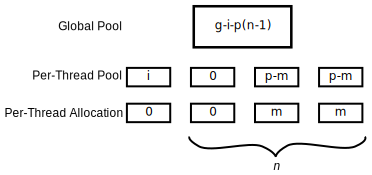
\includegraphics{SMPdesign/smpalloclim}}
	\end{center}
	\caption{Allocator Cache Run-Length Analysis}
	\label{fig:SMPdesign:Allocator Cache Run-Length Analysis}
	\end{figure}

	The relationships between these quantities is shown in
	Figure~\ref{fig:SMPdesign:Allocator Cache Run-Length Analysis}.
	The global pool is shown on the top of this figure, and
	the ``extra'' initializer thread's per-thread pool and
	per-thread allocations are the left-most pair of boxes.
	The initializer thread has no blocks allocated, but has
	$i$ blocks stranded in its per-thread pool.
	The rightmost two pairs of boxes are the per-thread pools and
	per-thread allocations of threads holding the maximum possible
	number of blocks, while the second-from-left pair of boxes
	represents the thread currently trying to allocate.

	The total number of blocks is $g$, and adding up the per-thread
	allocations and per-thread pools, we see that the global pool
	contains $g-i-p(n-1)$ blocks.
	If the allocating thread is to be successful, it needs at least
	$m$ blocks in the global pool, in other words:

	\begin{equation}
		g - i - p(n - 1) \ge m
	\label{sec:SMPdesign:g-vs-m}
	\end{equation}

	The question has $g=40$, $s=3$, and $n=2$.
	Equation~\ref{sec:SMPdesign:i} gives $i=4$, and
	Equation~\ref{sec:SMPdesign:p} gives $p=18$ for $m=18$
	and $p=21$ for $m=19$.
	Plugging these into Equation~\ref{sec:SMPdesign:g-vs-m}
	shows that $m=18$ will not overflow, but that $m=19$ might
	well do so.

	The presence of $i$ could be considered to be a bug.
	After all, why allocate memory only to have it stranded in
	the initialization thread's cache?
	One way of fixing this would be to provide a \co{memblock_flush()}
	function that flushed the current thread's pool into the
	global pool.
	The initialization thread could then invoke this function
	after freeing all of the blocks.

\QuickQAC{chp:Locking}{Locking}
\QuickQ{}
	Just how can serving as a whipping boy be considered to be
	in any way honorable???
\QuickA{}
	The reason locking serves as a research-paper whipping boy is
	because it is heavily used in practice.
	In contrast, if no one used or cared about locking, most research
	papers would not bother even mentioning it.

\QuickQ{}
	But the definition of deadlock only said that each thread
	was holding at least one lock and waiting on another lock
	that was held by some thread.
	How do you know that there is a cycle?
\QuickA{}
	Suppose that there is no cycle in the graph.
	We would then have a directed acyclic graph (DAG), which would
	have at least one leaf node.

	If this leaf node was a lock, then we would have a thread
	that was waiting on a lock that wasn't held by any thread,
	which violates the definition.
	(And in this case the thread would immediately acquire the
	lock.)

	On the other hand, if this leaf node was a thread, then
	we would have a thread that was not waiting on any lock,
	again violating the definition.
	(And in this case, the thread would either be running or
	be blocked on something that is not a lock.)

	Therefore, given this definition of deadlock, there must
	be a cycle in the corresponding graph.

\QuickQ{}
	Are there any exceptions to this rule, so that there really could be
	a deadlock cycle containing locks from both the library and
	the caller, even given that the library code never invokes
	any of the caller's functions?
\QuickA{}
	Indeed there are!
	Here are a few of them:
	\begin{enumerate}
	\item	If one of the library function's arguments is a pointer
		to a lock that this library function acquires, and if
		the library function holds one if its locks while
		acquiring the caller's lock, then we could have a
		deadlock cycle involving both caller and library locks.
	\item	If one of the library functions returns a pointer to
		a lock that is acquired by the caller, and if the
		caller acquires one if its locks while holding the
		library's lock, we could again have a deadlock
		cycle involving both caller and library locks.
	\item	If one of the library functions acquires a lock and
		then returns while still holding it, and if the caller
		acquires one of its locks, we have yet another way
		to create a deadlock cycle involving both caller
		and library locks.
	\item	If the caller has a signal handler that acquires
		locks, then the deadlock cycle can involve both
		caller and library locks.
		In this case, however, the library's locks are
		innocent bystanders in the deadlock cycle.
		That said, please note that acquiring a lock from
		within a signal handler is a no-no in most
		environments---it is not just a bad idea, it
		is unsupported.
	\end{enumerate}

\QuickQ{}
	But if \co{qsort()} releases all its locks before invoking
	the comparison function, how can it protect against races
	with other \co{qsort()} threads?
\QuickA{}
	By privatizing the data elements being compared
	(as discussed in Chapter~\ref{chp:Data Ownership})
	or through use of deferral mechanisms such as
	reference counting (as discussed in
	Chapter~\ref{chp:Deferred Processing}).

\QuickQ{}
	Name one common exception where it is perfectly reasonable
	to pass a pointer to a lock into a function.
\QuickA{}
	Locking primitives, of course!

\QuickQ{}
	Doesn't the fact that \co{pthread_cond_wait()} first releases the
	mutex and then re-acquires it eliminate the possibility of deadlock?
\QuickA{}
	Absolutely not!

	Consider the a program that acquires \co{mutex_a}, and then
	\co{mutex_b}, in that order, and then passes \co{mutex_a}
	to \co{pthread_cond_wait}.
	Now, \co{pthread_cond_wait} will release \co{mutex_a}, but
	will re-acquire it before returning.
	If some other thread acquires \co{mutex_a} in the meantime
	and then blocks on \co{mutex_b}, the program will deadlock.

\QuickQ{}
	Can the transformation from
	Figure~\ref{fig:locking:Protocol Layering and Deadlock} to
	Figure~\ref{fig:locking:Avoiding Deadlock Via Conditional Locking}
	be applied universally?
\QuickA{}
	Absolutely not!

	This transformation assumes that the
	\co{layer_2_processing()} function is idempotent, given that
	it might be executed multiple times on the same packet when
	the \co{layer_1()} routing decision changes.
	Therefore, in real life, this transformation can become
	arbitrarily complex.

\QuickQ{}
	But the complexity in
	Figure~\ref{fig:locking:Avoiding Deadlock Via Conditional Locking}
	is well worthwhile given that it avoids deadlock, right?
\QuickA{}
	Maybe.

	If the routing decision in \co{layer_1()} changes often enough,
	the code will always retry, never making forward progress.
	This is termed ``livelock'' if no thread makes any forward progress or
	``starvation''
	if some threads make forward progress but other do not
	(see Section~\ref{sec:locking:Livelock and Starvation}).

\QuickQ{}
	When using the ``acquire needed locks first'' approach described in
	Section~\ref{sec:locking:Acquire Needed Locks First},
	how can livelock be avoided?
\QuickA{}
	Provide an additional global lock.
	If a given thread has repeatedly tried and failed to acquire the needed
	locks, then have that thread unconditionally acquire the new
	global lock, and then unconditionally acquire any needed locks.
	(Suggested by Doug Lea.)

\QuickQ{}
	Why is it illegal to acquire a Lock~A that is acquired outside
	of a signal handler without blocking signals while holding
	a Lock~B that is acquired within a signal handler?
\QuickA{}
	Because this would lead to deadlock.
	Given that Lock~A is held outside of a signal
	handler without blocking signals, a signal might be handled while
	holding this lock.
	The corresponding signal handler might then acquire
	Lock~B, so that Lock~B is acquired while holding Lock~A.
	Therefore, if we also acquire Lock~A while holding Lock~B
	as called out in the question, we will have a deadlock cycle.

	Therefore, it is illegal to acquire a lock that is acquired outside
	of a signal handler without blocking signals while holding
	a another lock that is acquired within a signal handler.

\QuickQ{}
	How can you legally block signals within a signal handler?
\QuickA{}
	One of the simplest and fastest ways to do so is to use
	the \co{sa_mask} field of the \co{struct sigaction} that
	you pass to \co{sigaction()} when setting up the signal.

\QuickQ{}
	If acquiring locks in signal handlers is such a bad idea, why
	even discuss ways of making it safe?
\QuickA{}
	Because these same rules apply to the interrupt handlers used in
	operating-system kernels and in some embedded applications.

	In many application environments, acquiring locks in signal
	handlers is frowned upon~\cite{OpenGroup1997pthreads}.
	However, that does not stop clever developers from (usually
	unwisely) fashioning home-brew locks out of atomic operations.
	And atomic operations are in many cases perfectly legal in
	signal handlers.

\QuickQ{}
	Given an object-oriented application that passes control freely
	among a group of objects such that there is no straightforward
	locking hierarchy,\footnote{
		Also known as ``object-oriented spaghetti code.''}
	layered or otherwise, how can this
	application be parallelized?
\QuickA{}
	There are a number of approaches:
	\begin{enumerate}
	\item	In the case of parametric search via simulation,
		where a large number of simulations will be run
		in order to converge on (for example) a good design
		for a mechanical or electrical device, leave the
		simulation single-threaded, but run many instances
		of the simulation in parallel.
		This retains the object-oriented design, and
		gains parallelism at a higher level, and likely
		also avoids synchronization overhead.
	\item	Partition the objects into groups such that there
		is no need to operate on objects in
		more than one group at a given time.
		Then associate a lock with each group.
		This is an example of a single-lock-at-a-time
		design, which discussed in
		Section~\ref{sec:locking:Single-Lock-at-a-Time Designs}.
	\item	Partition the objects into groups such that threads
		can all operate on objects in the groups in some
		groupwise ordering.
		Then associate a lock with each group, and impose a
		locking hierarchy over the groups.
	\item	Impose an arbitrarily selected hierarchy on the locks,
		and then use conditional locking if it is necessary
		to acquire a lock out of order, as was discussed in
		Section~\ref{sec:locking:Conditional Locking}.
	\item	Before carrying out a given group of operations, predict
		which locks will be acquired, and attempt to acquire them
		before actually carrying out any updates.
		If the prediction turns out to be incorrect, drop
		all the locks and retry with an updated prediction
		that includes the benefit of experience.
		This approach was discussed in
		Section~\ref{sec:locking:Acquire Needed Locks First}.
	\item	Use transactional memory.
		This approach has a number of advantages and disadvantages
		which will be discussed in
		Section~\ref{sec:future:Transactional Memory}.
	\item	Refactor the application to be more concurrency-friendly.
		This would likely also have the side effect of making
		the application run faster even when single-threaded, but might
		also make it more difficult to modify the application.
	\item	Use techniques from later chapters in addition to locking.
	\end{enumerate}

\QuickQ{}
	How can the livelock shown in
	Figure~\ref{fig:locking:Abusing Conditional Locking}
	be avoided?
\QuickA{}
	Figure~\ref{fig:locking:Avoiding Deadlock Via Conditional Locking}
	provides some good hints.
	In many cases, livelocks are a hint that you should revisit your
	locking design.
	Or visit it in the first place if your locking design
	``just grew''.

	That said, one good-and-sufficient approach due to Doug Lea
	is to use conditional locking as described in
	Section~\ref{sec:locking:Conditional Locking}, but combine this
	with acquiring all needed locks first, before modifying shared
	data, as described in
	Section~\ref{sec:locking:Acquire Needed Locks First}.
	If a given critical section retries too many times,
	unconditionally acquire
	a global lock, then unconditionally acquire all the needed locks.
	This avoids both deadlock and livelock, and scales reasonably
	assuming that the global lock need not be acquired too often.

\QuickQ{}
	What problems can you spot in the code in
	Figure~\ref{fig:locking:Conditional Locking and Exponential Backoff}?
\QuickA{}
	Here are a couple:
	\begin{enumerate}
	\item	A one-second wait is way too long for most uses.
		Wait intervals should begin with roughly the time
		required to execute the critical section, which will
		normally be in the microsecond or millisecond range.
	\item	The code does not check for overflow.
		On the other hand, this bug is nullified
		by the previous bug: 32 bits worth of seconds is
		more than 50 years.
	\end{enumerate}

\QuickQ{}
	Wouldn't it be better just to use a good parallel design
	so that lock contention was low enough to avoid unfairness?
\QuickA{}
	It would be better in some sense, but there are situations
	where it can be appropriate to use
	designs that sometimes result in high lock contentions.

	For example, imagine a system that is subject to a rare error
	condition.
	It might well be best to have a simple error-handling design
	that has poor performance and scalability for the duration of
	the rare error condition, as opposed to a complex and
	difficult-to-debug design that is helpful only when one of
	those rare error conditions is in effect.

	That said, it is usually worth putting some effort into
	attempting to produce a design that both simple as well as
	efficient during error conditions, for example by partitioning
	the problem.

\QuickQ{}
	How might the lock holder be interfered with?
\QuickA{}
	If the data protected by the lock is in the same cache line
	as the lock itself, then attempts by other CPUs to acquire
	the lock will result in expensive cache misses on the part
	of the CPU holding the lock.
	This is a special case of false sharing, which can also occur
	if a pair of variables protected by different locks happen
	to share a cache line.
	In contrast, if the lock is in a different cache line than
	the data that it protects, the CPU holding the lock will
	usually suffer a cache miss only on first access to a given
	variable.

	Of course, the downside of placing the lock and data into separate
	cache lines is that the code will incur two cache misses rather
	than only one in the uncontended case.

\QuickQ{}
	Does it ever make sense to have an exclusive lock acquisition
	immediately followed by a release of that same lock, that is,
	an empty critical section?
\QuickA{}
	This usage is rare, but is occasionally used.
	The point is that the semantics of exclusive locks have two
	components: (1)~the familiar data-protection semantic and
	(2)~a messaging semantic, where releasing a given lock notifies
	a waiting acquisition of that same lock.
	An empty critical section uses the messaging component without
	the data-protection component.

	The rest of this answer provides some example uses of empty
	critical sections, however, these examples should be considered
	``gray magic.''\footnote{
		Thanks to Alexey Roytman for this decription.}
	As such, empty critical sections are almost never used in practice.
	Nevertheless, pressing on into this gray area...

	One historical use of empty critical sections appeared in the
	networking stack of the 2.4 Linux kernel.
	This usage pattern can be thought of as a way of approximating
	the effects of read-copy update (RCU), which is discussed in
	Section~\ref{sec:defer:Read-Copy Update (RCU)}.

	The empty-lock-critical-section idiom can also be used to
	reduce lock contention in some situations.
	For example, consider a multithreaded user-space application where
	each thread processes unit of work maintained in a per-thread
	list, where thread are prohibited from touching each others'
	lists.
	There could also be updates that require that all previously
	scheduled units of work have completed before the update can
	progress.
	One way to handle this is to schedule a unit of work on each
	thread, so that when all of these units of work complete, the
	update may proceed.

	In some applications, threads can come and go.
	For example, each thread might correspond to one user of the
	application, and thus be removed when that user logs out or
	otherwise disconnects.
	In many applications, threads cannot depart atomically: They must
	instead explicitly unravel themselves from various portions of
	the application using a specific sequence of actions.
	One specific action will be refusing to accept further requests
	from other threads, and another specific action will be disposing
	of any remaining units of work on its list, for example, by
	placing these units of work in a global work-item-disposal list
	to be taken by one of the remaining threads.
	(Why not just drain the thread's work-item list by executing
	each item?
	Because a given work item might generate more work items, so
	that the list could not be drained in a timely fashion.)

	If the application is to perform and scale well, a good locking
	design is required.
	One common solution is to have a global lock (call it \co{G})
	protecting the entire
	process of departing (and perhaps other things as well),
	with finer-grained locks protecting the
	individual unraveling operations.

	Now, a departing thread must clearly refuse to accept further
	requests before disposing of the work on its list, because
	otherwise additional work might arrive after the disposal action,
	which would render that disposal action ineffective.
	So simplified pseudocode for a departing thread might be as follows:

	\begin{enumerate}
	\item	Acquire lock \co{G}.
	\item	Acquire the lock guarding communications.
	\item	Refuse further communications from other threads.
	\item	Release the lock guarding communications.
	\item	Acquire the lock guarding the global work-item-disposal list.
	\item	Move all pending work items to the global
		work-item-disposal list.
	\item	Release the lock guarding the global work-item-disposal list.
	\item	Release lock \co{G}.
	\end{enumerate}

	Of course, a thread that needs to wait for all pre-existing work
	items will need to take departing threads into account.
	To see this, suppose that this thread starts waiting for all
	pre-existing work items just after a departing thread has refused
	further communications from other threads.
	How can this thread wait for the departing thread's work items
	to complete, keeping in mind that threads are not allowed to
	access each others' lists of work items?

	One straightforward approach is for this thread to acquire \co{G}
	and then the lock guarding the global work-item-disposal list, then
	move the work items to its own list.
	The thread then release both locks,
	places a work item on the end of it own list,
	and then wait for all of the work items that it placed on each thread's
	list (including its own) to complete.

	This approach does work well in many cases, but if special
	processing is required for each work item as it is pulled in
	from the global work-item-disposal list, the result could be
	excessive contention on \co{G}.
	One way to avoid that contention is to acquire \co{G} and then
	immediately release it.
	Then the process of waiting for all prior work items look
	something like the following:

	\begin{enumerate}
	\item	Set a global counter to one and initialize a condition
		variable to zero.
	\item	Send a message to all threads to cause them to atomically
		increment the global counter, and then to enqueue a
		work item.
		The work item will atomically decrement the global
		counter, and if the result is zero, it will set a
		condition variable to one.
	\item	Acquire \co{G}, which will wait on any currently departing
		thread to finish departing.
		Because only one thread may depart at a time, all the
		remaining threads will have already received the message
		sent in the preceding step.
	\item	Release \co{G}.
	\item	Acquire the lock guarding the global work-item-disposal list.
	\item	Move all work items from the global work-item-disposal list
		to this thread's list, processing them as needed along the way.
	\item	Release the lock guarding the global work-item-disposal list.
	\item	Enqueue an additional work item onto this thread's list.
		(As before, this work item will atomically decrement
		the global counter, and if the result is zero, it will
		set a condition variable to one.)
	\item	Wait for the condition variable to take on the value one.
	\end{enumerate}

	Once this procedure completes, all pre-existing work items are
	guaranteed to have completed.
	The empty critical sections are using locking for messaging as
	well as for protection of data.

\QuickQ{}
	Is there any other way for the VAX/VMS DLM to emulate
	a reader-writer lock?
\QuickA{}
	There are in fact several.
	One way would be to use the null, protected-read, and exclusive
	modes.
	Another way would be to use the null, protected-read, and
	concurrent-write modes.
	A third way would be to use the null, concurrent-read, and
	exclusive modes.

\QuickQ{}
	The code in
	Figure~\ref{fig:locking:Conditional Locking to Reduce Contention}
	is ridiculously complicated!
	Why not conditionally acquire a single global lock?
\QuickA{}
	Conditionally acquiring a single global lock does work very well,
	but only for relatively small numbers of CPUs.
	To see why it is problematic in systems with many hundreds of
	CPUs, look at
	Figure~\ref{fig:count:Atomic Increment Scalability on Nehalem}
	and extrapolate the delay from eight to 1,000 CPUs.

\QuickQ{}
	Wait a minute!
	If we ``win'' the tournament on line~16 of
	Figure~\ref{fig:locking:Conditional Locking to Reduce Contention},
	we get to do all the work of \co{do_force_quiescent_state()}.
	Exactly how is that a win, really?
\QuickA{}
	How indeed?
	This just shows that in concurrency, just as in life, one
	should take care to learn exactly what winning entails before
	playing the game.

\QuickQ{}
	Why not rely on the C language's default initialization of
	zero instead of using the explicit initializer shown on
	line~2 of
	Figure~\ref{fig:locking:Sample Lock Based on Atomic Exchange}?
\QuickA{}
	Because this default initialization does not apply to locks
	allocated as auto variables within the scope of a function.

\QuickQ{}
	Why bother with the inner loop on lines~7-8 of
	Figure~\ref{fig:locking:Sample Lock Based on Atomic Exchange}?
	Why not simply repeatedly do the atomic exchange operation
	on line~6?
\QuickA{}
	Suppose that the lock is held and that several threads
	are attempting to acquire the lock.
	In this situation, if these threads all loop on the atomic
	exchange operation, they will ping-pong the cache line
	containing the lock among themselves, imposing load
	on the interconnect.
	In contrast, if these threads are spinning in the inner
	loop on lines~7-8, they will each spin within their own
	caches, putting negligible load on the interconnect.

\QuickQ{}
	Why not simply store zero into the lock word on line 14 of
	Figure~\ref{fig:locking:Sample Lock Based on Atomic Exchange}?
\QuickA{}
	This can be a legitimate implementation, but only if
	this store is preceded by a memory barrier and makes use
	of \co{ACCESS_ONCE()}.
	The memory barrier is not required when the \co{xchg()}
	operation is used because this operation implies a
	full memory barrier due to the fact that it returns
	a value.

\QuickQ{}
	How can you tell if one counter is greater than another,
	while accounting for counter wrap?
\QuickA{}
	In the C language, the following macro correctly handles this:

\vspace{5pt}
\begin{minipage}[t]{\columnwidth}
\small
\begin{verbatim}
#define ULONG_CMP_LT(a, b) \
        (ULONG_MAX / 2 < (a) - (b))
\end{verbatim}
\end{minipage}
\vspace{5pt}

	Although it is tempting to simply subtract two signed integers,
	this should be avoided because signed overflow is undefined
	in the C language.
	For example, if the compiler knows that one of the values is
	positive and the other negative, it is within its rights to
	simply assume that the positive number is greater than the
	negative number, even though subtracting the negative number
	from the positive number might well result in overflow and
	thus a negative number.

	How could the compiler know the signs of the two numbers?
	It might be able to deduce it based on prior assignments
	and comparisons.
	In this case, if the per-CPU counters were signed, the compiler
	could deduce that they were always increasing in value, and
	then might assume that they would never go negative.
	This assumption could well lead the compiler to generate
	unfortunate code~\cite{PaulEMcKenney2012SignedOverflow,JohnRegehr2010UndefinedBehavior}.

\QuickQ{}
	Which is better, the counter approach or the flag approach?
\QuickA{}
	The flag approach will normally suffer fewer cache misses,
	but a better answer is to try both and see which works best
	for your particular workload.

\QuickQ{}
	How can relying on implicit existence guarantees result in
	a bug?
\QuickA{}
	Here are some bugs resulting from improper use of implicit
	existence guarantees:
	\begin{enumerate}
	\item	A program writes the address of a global variable to
		a file, then a later instance of that same program
		reads that address and attempts to dereference it.
		This can fail due to address-space randomization,
		to say nothing of recompilation of the program.
	\item	A module can record the address of one of its variables
		in a pointer located in some other module, then attempt
		to dereference that pointer after the module has
		been unloaded.
	\item	A function can record the address of one of its on-stack
		variables into a global pointer, which some other
		function might attempt to dereference after that function
		has returned.
	\end{enumerate}
	I am sure that you can come up with additional possibilities.

\QuickQ{}
	What if the element we need to delete is not the first element
	of the list on line~8 of
	Figure~\ref{fig:locking:Per-Element Locking Without Existence Guarantees}?
\QuickA{}
	This is a very simple hash table with no chaining, so the only
	element in a given bucket is the first element.
	The reader is invited to adapt this example to a hash table with
	full chaining.

\QuickQ{}
	What race condition can occur in
	Figure~\ref{fig:locking:Per-Element Locking Without Existence Guarantees}?
\QuickA{}
	Consider the following sequence of events:
	\begin{enumerate}
	\item	Thread~0 invokes \co{delete(0)}, and reaches line~10 of
		the figure, acquiring the lock.
	\item	Thread~1 concurrently invokes \co{delete(0)}, reaching
		line~10, but spins on the lock because Thread~0 holds it.
	\item	Thread~0 executes lines~11-14, removing the element from
		the hashtable, releasing the lock, and then freeing the
		element.
	\item	Thread~0 continues execution, and allocates memory, getting
		the exact block of memory that it just freed.
	\item	Thread~0 then initializes this block of memory as some
		other type of structure.
	\item	Thread~1's \co{spin_lock()} operation fails due to the
		fact that what it believes to be \co{p->lock} is no longer
		a spinlock.
	\end{enumerate}
	Because there is no existence guarantee, the identity of the
	data element can change while a thread is attempting to acquire
	that element's lock on line~10!

\QuickQAC{chp:Data Ownership}{Data Ownership}
\QuickQ{}
	What form of data ownership is extremely difficult
	to avoid when creating shared-memory parallel programs
	(for example, using pthreads) in C or C++?
\QuickA{}
	Use of auto variables in functions.
	By default, these are private to the thread executing the
	current function.

\QuickQ{}
	What synchronization remains in the example shown in
	Section~\ref{sec:owned:Multiple Processes}?
\QuickA{}
	The creation of the threads via the \co{sh} \co{&} operator
	and the joining of thread via the \co{sh} \co{wait}
	command.

	Of course, if the processes explicitly share memory, for
	example, using the \co{shmget()} or \co{mmap()} system
	calls, explicit synchronization might well be needed when
	acccessing or updating the shared memory.
	The processes might also synchronize using any of the following
	interprocess communications mechanisms:
	\begin{enumerate}
	\item	System V semaphores.
	\item	System V message queues.
	\item	UNIX-domain sockets.
	\item	Networking protocols, including TCP/IP, UDP, and a whole
		host of others.
	\item	File locking.
	\item	Use of the \co{open()} system call with the
		\co{O_CREAT} and \co{O_EXCL} flags.
	\item	Use of the \co{rename()} system call.
	\end{enumerate}
	A complete list of possible synchronization mechanisms is left
	as an exercise to the reader, who is warned that it will be
	an extremely long list.
	A surprising number of unassuming system calls can be pressed
	into service as synchronization mechanisms.

\QuickQ{}
	Is there any shared data in the example shown in
	Section~\ref{sec:owned:Multiple Processes}?
\QuickA{}
	That is a philosophical question.

	Those wishing the answer ``no'' might argue that processes by
	definition do not share memory.

	Those wishing to answer ``yes'' might list a large number of
	synchronization mechanisms that do not require shared memory,
	note that the kernel will have some shared state, and perhaps
	even argue that the assignment of process IDs (PIDs) constitute
	shared data.

	Such arguments are excellent intellectual exercise, and are
	also a wonderful way of feeling intelligent, scoring points
	against hapless classmates or colleagues,
	and (especially!) avoiding getting anything useful done.

\QuickQ{}
	Does it ever make sense to have partial data ownership where
	each thread reads only its own instance of a per-thread variable,
	but writes to other threads' instances?
\QuickA{}
	Amazingly enough, yes.
	One example is a simple message-passing system where threads post
	messages to other threads' mailboxes, and where each thread
	is responsible for removing any message it sent once that message
	has been acted on.
	Implementation of such an algorithm is left as an exercise for the
	reader, as is the task of identifying other algorithms with
	similar ownership patterns.

\QuickQ{}
	What mechanisms other than POSIX signals may be used for function
	shipping?
\QuickA{}
	There is a very large number of such mechanisms, including:
	\begin{enumerate}
	\item	System V message queues.
	\item	Shared-memory dequeue (see
		Section~\ref{sec:SMPdesign:Double-Ended Queue}).
	\item	Shared-memory mailboxes.
	\item	UNIX-domain sockets.
	\item	TCP/IP or UDP, possibly augmented by any number of
		higher-level protocols, including RPC, HTTP,
		XML, SOAP, and so on.
	\end{enumerate}
	Compilation of a complete list is left as an exercise to
	sufficiently single-minded readers, who are warned that the
	list will be extremely long.

\QuickQ{}
	But none of the data in the \co{eventual()} function shown on
	lines~15-32 of
	Figure~\ref{fig:count:Array-Based Per-Thread Eventually Consistent Counters}
	is actually owned by the \co{eventual()} thread!
	In just what way is this data ownership???
\QuickA{}
	The key phrase is ``owns the rights to the data''.
	In this case, the rights in question are the rights to access
	the per-thread \co{counter} variable defined on line~1
	of the figure.
	This situation is similar to that described in
	Section~\ref{sec:owned:Partial Data Ownership and pthreads}.

	However, there really is data that is owned by the \co{eventual()}
	thread, namely the \co{t} and \co{sum} variables defined on
	lines~17 and~18 of the figure.

	For other examples of designated threads, look at the kernel
	threads in the Linux kernel, for example, those created by
	\co{kthread_create()} and \co{kthread_run()}.

\QuickQ{}
	Is it possible to obtain greater accuracy while still
	maintaining full privacy of the per-thread data?
\QuickA{}
	Yes.
	One approach is for \co{read_count()} to add the value
	of its own per-thread variable.
	This maintains full ownership and performance, but only
	a slight improvement in accuracy, particulary on systems
	with very large numbers of threads.

	Another approach is for \co{read_count()} to use function
	shipping, for example, in the form of per-thread signals.
	This greatly improves accuracy, but at a significant performance
	cost for \co{read_count()}.

	However, both of these methods have the advantage of eliminating
	cache-line bouncing for the common case of updating counters.

\QuickQAC{chp:Deferred Processing}{Deferred Processing}
\QuickQ{}
	Why not implement reference-acquisition using
	a simple compare-and-swap operation that only
	acquires a reference if the reference counter is
	non-zero?
\QuickA{}
	Although this can resolve the race between the release of
	the last reference and acquisition of a new reference,
	it does absolutely nothing to prevent the data structure
	from being freed and reallocated, possibly as some completely
	different type of structure.
	It is quite likely that the ``simple compare-and-swap
	operation'' would give undefined results if applied to the
	differently typed structure.

	In short, use of atomic operations such as compare-and-swap
	absolutely requires either type-safety or existence guarantees.

\QuickQ{}
	Why isn't it necessary to guard against cases where one CPU
	acquires a reference just after another CPU releases the last
	reference?
\QuickA{}
	Because a CPU must already hold a reference in order
	to legally acquire another reference.
	Therefore, if one CPU releases the last reference,
	there cannot possibly be any CPU that is permitted
	to acquire a new reference.
	This same fact allows the non-atomic check in line~22
	of Figure~\ref{fig:defer:Linux Kernel kref API}.

\QuickQ{}
	Suppose that just after the \co{atomic_sub_and_test()}
	on line~22 of
	Figure~\ref{fig:defer:Linux Kernel kref API} is invoked,
	that some other CPU invokes \co{kref_get()}.
	Doesn't this result in that other CPU now having an illegal
	reference to a released object?
\QuickA{}
	This cannot happen if these functions are used correctly.
	It is illegal to invoke \co{kref_get()} unless you already
	hold a reference, in which case the \co{kref_sub()} could
	not possibly have decremented the counter to zero.

\QuickQ{}
	Suppose that \co{kref_sub()} returns zero, indicating that
	the \co{release()} function was not invoked.
	Under what conditions can the caller rely on the continued
	existence of the enclosing object?
\QuickA{}
	The caller cannot rely on the continued existence of the
	object unless it knows that at least one reference will
	continue to exist.
	Normally, the caller will have no way of knowing this, and
	must therefore carefullly avoid referencing the object after
	the call to \co{kref_sub()}.

\QuickQ{}
	Why not just pass \co{kfree()} as the release function?
\QuickA{}
	Because the \co{kref} structure normally is embedded in
	a larger structure, and it is necessary to free the entire
	structure, not just the \co{kref} field.
	This is normally accomplished by defining a wrapper function
	that does a \co{container_of()} and then a \co{kfree()}.

\QuickQ{}
	Why can't the check for a zero reference count be
	made in a simple ``if'' statement with an atomic
	increment in its ``then'' clause?
\QuickA{}
	Suppose that the ``if'' condition completed, finding
	the reference counter value equal to one.
	Suppose that a release operation executes, decrementing
	the reference counter to zero and therefore starting
	cleanup operations.
	But now the ``then'' clause can increment the counter
	back to a value of one, allowing the object to be
	used after it has been cleaned up.

\QuickQ{}
	Why does \co{hp_store()} in
	Figure~\ref{fig:defer:Hazard-Pointer Storage and Erasure}
	take a double indirection to the data element?
	Why not \co{void *} instead of \co{void **}?
\QuickA{}
	Because \co{hp_record()} must check for concurrent modifications.
	To do that job, it needs a pointer to a pointer to the element,
	so that it can check for a modification to the pointer to the
	element.

\QuickQ{}
	Why does \co{hp_store()}'s caller need to restart its
	traversal from the beginning in case of failure?
	Isn't that inefficient for large data structures?
\QuickA{}
	It might be inefficient in some sense, but the fact is that
	such restarting is absolutely required for correctness.
	To see this, consider a hazard-pointer-protected linked list
	containing elements~A, B, and~C that is subjecte to the
	following sequence of events:

	\begin{enumerate}
	\item	Thread~0 stores a hazard pointer to element~B
		(having presumably traversed to element~B from element~A).
	\item	Thread~1 removes element~B from the list, which sets
		the pointer from element~B to element~C to a special
		\co{HAZPTR_POISON} value in order to mark the deletion.
		Because Thread~0 has a hazard pointer to element~B,
		it cannot yet be freed.
	\item	Thread~1 removes element~C from the list.
		Because there are no hazard pointers referencing element~C,
		it is immediately freed.
	\item	Thread~0 attempts to acquire a hazard pointer to
		now-removed element~B's successor, but sees the
		\co{HAZPTR_POISON} value, and thus returns zero,
		forcing the caller to restart its traversal from the
		beginning of the list.
	\end{enumerate}

	Which is a very good thing, because otherwise Thread~0 would
	have attempted to access the now-freed element~C,
	which might have resulted in arbitrarily horrible
	memory corruption, especially if the memory for
	element~C had since been re-allocated for some other
	purpose.

\QuickQ{}
	Given that papers on hazard pointers use the bottom bits
	of each pointer to mark deleted elements, what is up with
	\co{HAZPTR_POISON}?
\QuickA{}
	The published implementations of hazard pointers used
	non-blocking synchornization techniques for insertion
	and deletion.
	These techniques require that readers traversing the
	data structure ``help'' updaters complete their updates,
	which in turn means that readers need to look at the successor
	of a deleted element.

	In contrast, we will be using locking to synchronize updates,
	which does away with the need for readers to help updaters
	complete their updates, which in turn allows us to leave
	pointers' bottom bits alone.
	This approach allows read-side code to be simpler and faster.

\QuickQ{}
	But don't these restrictions on hazard pointers also apply
	to other forms of reference counting?
\QuickA{}
	These restrictions apply only to reference-counting mechanisms whose
	reference acquisition can fail.

\QuickQ{}
	An \co{atomic_read()} and an \co{atomic_set()} that are
	non-atomic?
	Is this some kind of bad joke???
\QuickA{}
	It might well seem that way, but in situations where no other
	CPU has access to the atomic variable in question, the overhead
	of an actual atomic instruction would be wasteful.
	Two examples where no other CPU has access are
	during initialization and cleanup.

\QuickQ{}
	But hazard pointers don't write to the data structure!
\QuickA{}
	Indeed, they do not.
	However, they do write to the hazard pointers themselves,
	and, more important, require that possible failures be
	handled for all \co{hp_store()} calls, each of which
	might fail.
	Therefore, although hazard pointers are extremely useful,
	it is still worth looking for improved mechanisms.

\QuickQ{}
	Why isn't this sequence-lock discussion in Chapter~\ref{chp:Locking},
	you know, the one on \emph{locking}?
\QuickA{}
	The sequence-lock mechanism is really a combination of two
	separate synchronization mechanisms, sequence counts and
	locking.
	In fact, the sequence-count mechanism is available separately
	in the Linux kernel via the
	\co{write_seqcount_begin()} and \co{write_seqcount_end()}
	primitives.

	However, the combined \co{write_seqlock()} and
	\co{write_sequnlock()} primitives are used much more heavily
	in the Linux kernel.
	More importantly, many more people will understand what you
	mean if you say ``sequence lock'' than if you say
	``sequence count''.

	So this section is entitled ``Sequence Locks'' so that people
	will understand what it is about just from the title, and
	it appears in the ``Deferred Processing'' because (1) of the
	emphasis on the ``sequence count'' aspect of ``sequence locks''
	and (2) because a ``sequence lock'' is much more than merely
	a lock.

\QuickQ{}
	Can you use sequence locks as the only synchronization
	mechanism protecting a linked list supporting concurrent
	addition, deletion, and search?
\QuickA{}
	One trivial way of accomplishing this is to surround all
	accesses, including the read-only accesses, with
	\co{write_seqlock()} and \co{write_sequnlock()}.
	Of course, this solution also prohibits all read-side
	parallelism, and furthermore could just as easily be implemented
	using simple locking.

	If you do come up with a solution that uses \co{read_seqbegin()}
	and \co{read_seqretry()} to protect read-side accesses, make
	sure that you correctly handle the following sequence of events:

	\begin{enumerate}
	\item	CPU~0 is traversing the linked list, and picks up a pointer
		to list element~A.
	\item	CPU~1 removes element~A from the list and frees it.
	\item	CPU~2 allocates an unrelated data structure, and gets
		the memory formerly occupied by element~A.
		In this unrelated data structure, the memory previously
		used for element~A's \co{->next} pointer is now occupied
		by a floating-point number.
	\item	CPU~0 picks up what used to be element~A's \co{->next}
		pointer, gets random bits, and therefore gets a
		segmentation fault.
	\end{enumerate}

	One way to protect against this sort of problem requires use
	of ``type-safe memory'', which will be discussed in
	Section~\ref{sec:defer:RCU is a Way of Providing Type-Safe Memory}.
	But in that case, you would be using some other synchronization
	mechanism in addition to sequence locks!

\QuickQ{}
	Why bother with the check on line~19 of
	\co{read_seqbegin()} in
	Figure~\ref{fig:defer:Sequence-Locking Implementation}?
	Given that a new writer could begin at any time, why not
	simply incorporate the check into line~31 of
	\co{read_seqretry()}?
\QuickA{}
	That would be a legitimate implementation.
	However, it would not save anything to move the check down
	to \co{read_seqretry()}: There would be roughly the same number
	of instructions.
	Furthermore, the reader's accesses from its doomed read-side
	critical section could inflict overhead on the writer in
	the form of cache misses.
	We can avoid these cache misses by placing the check in
	\co{read_seqbegin()} as shown on line~19 of
	Figure~\ref{fig:defer:Sequence-Locking Implementation}.

\QuickQ{}
	Why is the \co{smp_mb()} on line~29 of
	Figure~\ref{fig:defer:Sequence-Locking Implementation}
	needed?
\QuickA{}
	If it was omitted, both the compiler and the CPU would be
	within their rights to move the critical section preceding
	the call to \co{read_seqretry()} down below this function.
	This would prevent the sequence lock from protecting the
	critical section.
	The \co{smp_mb()} primitive prevents such reordering.

\QuickQ{}
	Can't weaker memory barriers be used in the code in
	Figure~\ref{fig:defer:Sequence-Locking Implementation}?
\QuickA{}
	In older versions of the Linux kernel, no.

	In very new versions of the Linux kernel, line~17 could use
	\co{smp_load_acquire()} instead of \co{ACCESS_ONCE()}, which
	in turn would allow the \co{smp_mb()} on line~18 to be dropped.
	Similarly, line~44 could use an \co{smp_store_release()}, for
	example, as follows: \\
	\co{smp_store_release(&slp->seq, ACCESS_ONCE(slp->seq) + 1);} \\
	This would allow the \co{smp_mb()} on line~43 to be dropped.

\QuickQ{}
	What prevents sequence-locking updaters from starving readers?
\QuickA{}
	Nothing.
	This is one of the weaknesses of sequence locking, and as a
	result, you should use sequence locking only in read-mostly
	situations.
	Unless of course read-side starvation is acceptable in your
	situation, in which case, go wild with the sequence-locking updates!

\QuickQ{}
	What if something else serializes writers, so that the lock
	is not needed?
\QuickA{}
	In this case, the \co{->lock} field could be omitted, as it
	is in \co{seqcount_t} in the Linux kernel.

\QuickQ{}
	Why isn't \co{seq} on line 2 of
	Figure~\ref{fig:defer:Sequence-Locking Implementation}
	\co{unsigned} rather than \co{unsigned long}?
	After all, if \co{unsigned} is good enough for the Linux
	kernel, shouldn't it be good enough for everyone?
\QuickA{}
	Not at all.
	The Linux kernel has a number of special attributes that allow
	it to ignore the following sequence of events:
	\begin{enumerate}
	\item	Thread 0 executes \co{read_seqbegin()}, picking up
		\co{->seq} in line~17, noting that the value is even,
		and thus returning to the caller.
	\item	Thread 0 starts executing its read-side critical section,
		but is then preempted for a long time.
	\item	Other threads repeatedly invoke \co{write_seqlock()} and
		\co{write_sequnlock()}, until the value of \co{->seq}
		overflows back to the value that Thread~0 fetched.
	\item	Thread 0 resumes execution, completing its read-side
		critical section with inconsistent data.
	\item	Thread 0 invokes \co{read_seqretry()}, which incorrectly
		concludes that Thread~0 has seen a consistent view of
		the data protected by the sequence lock.
	\end{enumerate}

	The Linux kernel uses sequence locking for things that are
	updated rarely, with time-of-day information being a case
	in point.
	This information is updated at most once per millisecond,
	so that seven weeks would be required to overflow the counter.
	If a kernel thread was preempted for seven weeks, the Linux
	kernel's soft-lockup code would be emitting warnings every two
	minutes for that entire time.

	In contrast, with a 64-bit counter, more than five centuries
	would be required to overflow, even given an update every
	\emph{nano}second.
	Therefore, this implementation uses a type for \co{->seq}
	that is 64 bits on 64-bit systems.

\QuickQ{}
	But doesn't Section~\ref{sec:defer:Sequence Locks}'s seqlock
	also permit readers and updaters to get work done concurrently?
\QuickA{}
	Yes and no.
	Although seqlock readers can run concurrently with
	seqlock writers, whenever this happens, the {\tt read\_seqretry()}
	primitive will force the reader to retry.
	This means that any work done by a seqlock reader running concurrently
	with a seqlock updater will be discarded and redone.
	So seqlock readers can \emph{run} concurrently with updaters,
	but they cannot actually get any work done in this case.

	In contrast, RCU readers can perform useful work even in presence
	of concurrent RCU updaters.

\QuickQ{}
	What prevents the {\tt list\_for\_each\_entry\_rcu()} from
	getting a segfault if it happens to execute at exactly the same
	time as the {\tt list\_add\_rcu()}?
\QuickA{}
	On all systems running Linux, loads from and stores
	to pointers are atomic, that is, if a store to a pointer occurs at
	the same time as a load from that same pointer, the load will return
	either the initial value or the value stored, never some bitwise
	mashup of the two.
	In addition, the {\tt list\_for\_each\_entry\_rcu()} always proceeds
	forward through the list, never looking back.
	Therefore, the {\tt list\_for\_each\_entry\_rcu()} will either see
	the element being added by {\tt list\_add\_rcu()} or it will not,
	but either way, it will see a valid well-formed list.

\QuickQ{}
	Why do we need to pass two pointers into
	{\tt hlist\_for\_each\_entry\_rcu()}
	when only one is needed for {\tt list\_for\_each\_entry\_rcu()}?
\QuickA{}
	Because in an hlist it is necessary to check for
	NULL rather than for encountering the head.
	(Try coding up a single-pointer {\tt hlist\_for\_each\_entry\_rcu()}
	If you come up with a nice solution, it would be a very good thing!)

\QuickQ{}
	How would you modify the deletion example to permit more than two
	versions of the list to be active?
\QuickA{}
	One way of accomplishing this is as shown in
	Figure~\ref{fig:defer:Concurrent RCU Deletion}.

\begin{figure}[htbp]
{ \centering
\begin{verbatim}
  1 spin_lock(&mylock);
  2 p = search(head, key);
  3 if (p == NULL)
  4   spin_unlock(&mylock);
  5 else {
  6   list_del_rcu(&p->list);
  7   spin_unlock(&mylock);
  8   synchronize_rcu();
  9   kfree(p);
 10 }
\end{verbatim}
}
\caption{Concurrent RCU Deletion}
\label{fig:defer:Concurrent RCU Deletion}
\end{figure}

	Note that this means that multiple concurrent deletions might be
	waiting in \co{synchronize_rcu()}.

\QuickQ{}
	How many RCU versions of a given list can be
	active at any given time?
\QuickA{}
	That depends on the synchronization design.
	If a semaphore protecting the update is held across the grace period,
	then there can be at most two versions, the old and the new.

	However, suppose that only the search, the update, and the
	\co{list_replace_rcu()} were protected by a lock, so that
	the \co{synchronize_rcu()} was outside of that lock, similar
	to the code shown in
	Figure~\ref{fig:defer:Concurrent RCU Deletion}.
	Suppose further that a large number of threads undertook an
	RCU replacement at about the same time, and that readers
	are also constantly traversing the data structure.

	Then the following sequence of events could occur, starting from
	the end state of
	Figure~\ref{fig:defer:RCU Replacement in Linked List}:

	\begin{enumerate}
	\item	Thread~A traverses the list, obtaining a reference to
		the 5,2,3 element.
	\item	Thread~B replaces the 5,2,3 element with a new
		5,2,4 element, then waits for its \co{synchronize_rcu()}
		call to return.
	\item	Thread~C traverses the list, obtaining a reference to
		the 5,2,4 element.
	\item	Thread~D replaces the 5,2,4 element with a new
		5,2,5 element, then waits for its \co{synchronize_rcu()}
		call to return.
	\item	Thread~E traverses the list, obtaining a reference to
		the 5,2,5 element.
	\item	Thread~F replaces the 5,2,5 element with a new
		5,2,6 element, then waits for its \co{synchronize_rcu()}
		call to return.
	\item	Thread~G traverses the list, obtaining a reference to
		the 5,2,6 element.
	\item	And the previous two steps repeat quickly, so that all
		of them happen before any of the \co{synchronize_rcu()}
		calls return.
	\end{enumerate}

	Thus, there can be an arbitrary number of versions active,
	limited only by memory and by how many updates could be completed
	within a grace period.
	But please note that data structures that are updated so frequently
	probably are not good candidates for RCU.
	That said, RCU can handle high update rates when necessary.

\QuickQ{}
	How can RCU updaters possibly delay RCU readers, given that the
	{\tt rcu\_read\_lock()} and {\tt rcu\_read\_unlock()}
	primitives neither spin nor block?
\QuickA{}
	The modifications undertaken by a given RCU updater will cause the
	corresponding CPU to invalidate cache lines containing the data,
	forcing the CPUs running concurrent RCU readers to incur expensive
	cache misses.
	(Can you design an algorithm that changes a data structure
	\emph{without}
	inflicting expensive cache misses on concurrent readers?
	On subsequent readers?)

\QuickQ{}
	WTF?
	How the heck do you expect me to believe that RCU has a
	100-femtosecond overhead when the clock period at 3GHz is more than
	300 \emph{picoseconds}?
\QuickA{}
	First, consider that the inner loop used to
	take this measurement is as follows:

\vspace{5pt}
\begin{minipage}[t]{\columnwidth}
\scriptsize
\begin{verbatim}
  1 for (i = 0; i < CSCOUNT_SCALE; i++) {
  2   rcu_read_lock();
  3   rcu_read_unlock();
  4 }
\end{verbatim}
\end{minipage}
\vspace{5pt}

	Next, consider the effective definitions of \co{rcu_read_lock()}
	and \co{rcu_read_unlock()}:

\vspace{5pt}
\begin{minipage}[t]{\columnwidth}
\scriptsize
\begin{verbatim}
  1 #define rcu_read_lock()   do { } while (0)
  2 #define rcu_read_unlock() do { } while (0)
\end{verbatim}
\end{minipage}
\vspace{5pt}

	Consider also that the compiler does simple optimizations,
	allowing it to replace the loop with:

\vspace{5pt}
\begin{minipage}[t]{\columnwidth}
\scriptsize
\begin{verbatim}
i = CSCOUNT_SCALE;
\end{verbatim}
\end{minipage}
\vspace{5pt}

	So the ``measurement'' of 100 femtoseconds is simply the fixed
	overhead of the timing measurements divided by the number of
	passes through the inner loop containing the calls
	to \co{rcu_read_lock()} and \co{rcu_read_unlock()}.
	And therefore, this measurement really is in error, in fact,
	in error by an arbitrary number of orders of magnitude.
	As you can see by the definition of \co{rcu_read_lock()}
	and \co{rcu_read_unlock()} above, the actual overhead
	is precisely zero.

	It certainly is not every day that a timing measurement of
	100 femtoseconds turns out to be an overestimate!

\QuickQ{}
	Why does both the variability and overhead of rwlock decrease as the
	critical-section overhead increases?
\QuickA{}
	Because the contention on the underlying
	\co{rwlock_t} decreases as the critical-section overhead
	increases.
	However, the rwlock overhead will not quite drop to that on a single
	CPU because of cache-thrashing overhead.

\QuickQ{}
	Is there an exception to this deadlock immunity, and if so,
	what sequence of events could lead to deadlock?
\QuickA{}
	One way to cause a deadlock cycle involving
	RCU read-side primitives is via the following (illegal) sequence
	of statements:

\vspace{5pt}
\begin{minipage}[t]{\columnwidth}
\small
\begin{verbatim}
idx = srcu_read_lock(&srcucb);
synchronize_srcu(&srcucb);
srcu_read_unlock(&srcucb, idx);
\end{verbatim}
\end{minipage}
\vspace{5pt}

	The \co{synchronize_srcu()} cannot return until all
	pre-existing SRCU read-side critical sections complete, but
	is enclosed in an SRCU read-side critical section that cannot
	complete until the \co{synchronize_srcu()} returns.
	The result is a classic self-deadlock--you get the same
	effect when attempting to write-acquire a reader-writer lock
	while read-holding it.

	Note that this self-deadlock scenario does not apply to
	RCU Classic, because the context switch performed by the
	\co{synchronize_rcu()} would act as a quiescent state
	for this CPU, allowing a grace period to complete.
	However, this is if anything even worse, because data used
	by the RCU read-side critical section might be freed as a
	result of the grace period completing.

	In short, do not invoke synchronous RCU update-side primitives
	from within an RCU read-side critical section.

\QuickQ{}
	Immunity to both deadlock and priority inversion???
	Sounds too good to be true.
	Why should I believe that this is even possible?
\QuickA{}
	It really does work.
	After all, if it didn't work, the Linux kernel would not run.

\QuickQ{}
	But wait!
	This is exactly the same code that might be used when thinking
	of RCU as a replacement for reader-writer locking!
	What gives?
\QuickA{}
	This is an effect of the Law of Toy Examples:
	beyond a certain point, the code fragments look the same.
	The only difference is in how we think about the code.
	However, this difference can be extremely important.
	For but one example of the importance, consider that if we think
	of RCU as a restricted reference counting scheme, we would never
	be fooled into thinking that the updates would exclude the RCU
	read-side critical sections.

	It nevertheless is often useful to think of RCU as a replacement
	for reader-writer locking, for example, when you are replacing
	reader-writer locking with RCU.

\QuickQ{}
	Why the dip in refcnt overhead near 6 CPUs?
\QuickA{}
	Most likely NUMA effects.
	However, there is substantial variance in the values measured for the
	refcnt line, as can be seen by the error bars.
	In fact, standard deviations range in excess of 10\% of measured
	values in some cases.
	The dip in overhead therefore might well be a statistical aberration.

\QuickQ{}
	What if the element we need to delete is not the first element
	of the list on line~9 of
	Figure~\ref{fig:defer:Existence Guarantees Enable Per-Element Locking}?
\QuickA{}
	As with
	Figure~\ref{fig:locking:Per-Element Locking Without Existence Guarantees},
	this is a very simple hash table with no chaining, so the only
	element in a given bucket is the first element.
	The reader is again invited to adapt this example to a hash table with
	full chaining.

\QuickQ{}
	Why is it OK to exit the RCU read-side critical section on
	line~15 of
	Figure~\ref{fig:defer:Existence Guarantees Enable Per-Element Locking}
	before releasing the lock on line~17?
\QuickA{}
	First, please note that the second check on line~14 is
	necessary because some other
	CPU might have removed this element while we were waiting
	to acquire the lock.
	However, the fact that we were in an RCU read-side critical section
	while acquiring the lock guarantees that this element could not
	possibly have been re-allocated and re-inserted into this
	hash table.
	Furthermore, once we acquire the lock, the lock itself guarantees
	the element's existence, so we no longer need to be in an
	RCU read-side critical section.

	The question as to whether it is necessary to re-check the
	element's key is left as an exercise to the reader.
	% A re-check is necessary if the key can mutate or if it is
	% necessary to reject deleted entries (in cases where deletion
	% is recorded by mutating the key.

\QuickQ{}
	Why not exit the RCU read-side critical section on
	line~23 of
	Figure~\ref{fig:defer:Existence Guarantees Enable Per-Element Locking}
	before releasing the lock on line~22?
\QuickA{}
	Suppose we reverse the order of these two lines.
	Then this code is vulnerable to the following sequence of
	events:
	\begin{enumerate}
	\item	CPU~0 invokes \co{delete()}, and finds the element
		to be deleted, executing through line~15.
		It has not yet actually deleted the element, but
		is about to do so.
	\item	CPU~1 concurrently invokes \co{delete()}, attempting
		to delete this same element.
		However, CPU~0 still holds the lock, so CPU~1 waits
		for it at line~13.
	\item	CPU~0 executes lines~16 and 17, and blocks at
		line~18 waiting for CPU~1 to exit its RCU read-side
		critical section.
	\item	CPU~1 now acquires the lock, but the test on line~14
		fails because CPU~0 has already removed the element.
		CPU~1 now executes line~22 (which we switched with line~23
		for the purposes of this Quick Quiz)
		and exits its RCU read-side critical section.
	\item	CPU~0 can now return from \co{synchronize_rcu()},
		and thus executes line~19, sending the element to
		the freelist.
	\item	CPU~1 now attempts to release a lock for an element
		that has been freed, and, worse yet, possibly
		reallocated as some other type of data structure.
		This is a fatal memory-corruption error.
	\end{enumerate}

\QuickQ{}
	But what if there is an arbitrarily long series of RCU
	read-side critical sections in multiple threads, so that at
	any point in time there is at least one thread in the system
	executing in an RCU read-side critical section?
	Wouldn't that prevent any data from a \co{SLAB_DESTROY_BY_RCU}
	slab ever being returned to the system, possibly resulting
	in OOM events?
\QuickA{}
	There could certainly be an arbitrarily long period of time
	during which at least one thread is always in an RCU read-side
	critical section.
	However, the key words in the description in
	Section~\ref{sec:defer:RCU is a Way of Providing Type-Safe Memory}
	are ``in-use'' and ``pre-existing''.
	Keep in mind that a given RCU read-side critical section is
	conceptually only permitted to gain references to data elements
	that were in use at the beginning of that critical section.
	Furthermore, remember that a slab cannot be returned to the
	system until all of its data elements have been freed, in fact,
	the RCU grace period cannot start until after they have all been
	freed.

	Therefore, the slab cache need only wait for those RCU read-side
	critical sections that started before the freeing of the last element
	of the slab.
	This in turn means that any RCU grace period that begins after
	the freeing of the last element will do---the slab may be returned
	to the system after that grace period ends.

\QuickQ{}
	Suppose that the \co{nmi_profile()} function was preemptible.
	What would need to change to make this example work correctly?
\QuickA{}
	One approach would be to use
	\co{rcu_read_lock()} and \co{rcu_read_unlock()}
	in \co{nmi_profile()}, and to replace the
	\co{synchronize_sched()} with \co{synchronize_rcu()},
	perhaps as shown in
	Figure~\ref{fig:defer:Using RCU to Wait for Mythical Preemptible NMIs to Finish}.

\begin{figure}[tbp]
{ \tt \scriptsize
\begin{verbatim}
  1 struct profile_buffer {
  2   long size;
  3   atomic_t entry[0];
  4 };
  5 static struct profile_buffer *buf = NULL;
  6
  7 void nmi_profile(unsigned long pcvalue)
  8 {
  9   struct profile_buffer *p;
 10
 11   rcu_read_lock();
 12   p = rcu_dereference(buf);
 13   if (p == NULL) {
 14     rcu_read_unlock();
 15     return;
 16   }
 17   if (pcvalue >= p->size) {
 18     rcu_read_unlock();
 19     return;
 20   }
 21   atomic_inc(&p->entry[pcvalue]);
 22   rcu_read_unlock();
 23 }
 24
 25 void nmi_stop(void)
 26 {
 27   struct profile_buffer *p = buf;
 28
 29   if (p == NULL)
 30     return;
 31   rcu_assign_pointer(buf, NULL);
 32   synchronize_rcu();
 33   kfree(p);
 34 }
\end{verbatim}
}
\caption{Using RCU to Wait for Mythical Preemptible NMIs to Finish}
\label{fig:defer:Using RCU to Wait for Mythical Preemptible NMIs to Finish}
\end{figure}


\QuickQ{}
	Why do some of the cells in
	Table~\ref{tab:defer:RCU Wait-to-Finish APIs}
	have exclamation marks (``!'')?
\QuickA{}
	The API members with exclamation marks (\co{rcu_read_lock()},
	\co{rcu_read_unlock()}, and \co{call_rcu()}) were the
	only members of the Linux RCU API that Paul E. McKenney was aware
	of back in the mid-90s.
	During this timeframe, he was under the mistaken impression that
	he knew all that there is to know about RCU.

\QuickQ{}
	How do you prevent a huge number of RCU read-side critical
	sections from indefinitely blocking a \co{synchronize_rcu()}
	invocation?
\QuickA{}
	There is no need to do anything to prevent RCU read-side
	critical sections from indefinitely blocking a
	\co{synchronize_rcu()} invocation, because the
	\co{synchronize_rcu()} invocation need wait only for
	\emph{pre-existing} RCU read-side critical sections.
	So as long as each RCU read-side critical section is
	of finite duration, there should be no problem.

\QuickQ{}
	The \co{synchronize_rcu()} API waits for all pre-existing
	interrupt handlers to complete, right?
\QuickA{}
	Absolutely not!
	And especially not when using preemptible RCU!
	You instead want \co{synchronize_irq()}.
	Alternatively, you can place calls to \co{rcu_read_lock()}
	and \co{rcu_read_unlock()} in the specific interrupt handlers that
	you want \co{synchronize_rcu()} to wait for.

\QuickQ{}
	What happens if you mix and match?
	For example, suppose you use \co{rcu_read_lock()} and
	\co{rcu_read_unlock()} to delimit RCU read-side critical
	sections, but then use \co{call_rcu_bh()} to post an
	RCU callback?
\QuickA{}
	If there happened to be no RCU read-side critical
	sections delimited by \co{rcu_read_lock_bh()} and
	\co{rcu_read_unlock_bh()} at the time \co{call_rcu_bh()}
	was invoked, RCU would be within its rights to invoke the callback
	immediately, possibly freeing a data structure still being used by
	the RCU read-side critical section!
	This is not merely a theoretical possibility: a long-running RCU
	read-side critical section delimited by \co{rcu_read_lock()}
	and \co{rcu_read_unlock()} is vulnerable to this failure mode.

	However, the \co{rcu_dereference()} family of functions apply
	to all flavors of RCU.
	(There was an attempt to have per-flavor variants of
	\co{rcu_dereference()}, but it was just too messy.)

\QuickQ{}
	Hardware interrupt handlers can be thought of as being
	under the protection of an implicit \co{rcu_read_lock_bh()},
	right?
\QuickA{}
	Absolutely not!
	And especially not when using preemptible RCU!
	If you need to access ``rcu\_bh''-protected data structures
	in an interrupt handler, you need to provide explicit calls to
	\co{rcu_read_lock_bh()} and \co{rcu_read_unlock_bh()}.

\QuickQ{}
	What happens if you mix and match RCU Classic and RCU Sched?
\QuickA{}
	In a non-\co{PREEMPT} or a \co{PREEMPT} kernel, mixing these
	two works ``by accident'' because in those kernel builds, RCU Classic
	and RCU Sched map to the same implementation.
	However, this mixture is fatal in \co{PREEMPT_RT} builds using the -rt
	patchset, due to the fact that Realtime RCU's read-side critical
	sections can be preempted, which would permit
	\co{synchronize_sched()} to return before the
	RCU read-side critical section reached its \co{rcu_read_unlock()}
	call.
	This could in turn result in a data structure being freed before the
	read-side critical section was finished with it,
	which could in turn greatly increase the actuarial risk experienced
	by your kernel.

	In fact, the split between RCU Classic and RCU Sched was inspired
	by the need for preemptible RCU read-side critical sections.

\QuickQ{}
	In general, you cannot rely on \co{synchronize_sched()} to
	wait for all pre-existing interrupt handlers,
	right?
\QuickA{}
	That is correct!
	Because -rt Linux uses threaded interrupt handlers, there can
	be context switches in the middle of an interrupt handler.
	Because \co{synchronize_sched()} waits only until each
	CPU has passed through a context switch, it can return
	before a given interrupt handler completes.

	If you need to wait for a given interrupt handler to complete,
	you should instead use \co{synchronize_irq()} or place
	explicit RCU read-side critical sections in the interrupt
	handlers that you wish to wait on.

\QuickQ{}
	Why do both SRCU and QRCU lack asynchronous \co{call_srcu()}
	or \co{call_qrcu()} interfaces?
\QuickA{}
	Given an asynchronous interface, a single task
	could register an arbitrarily large number of SRCU or QRCU callbacks,
	thereby consuming an arbitrarily large quantity of memory.
	In contrast, given the current synchronous
	\co{synchronize_srcu()} and \co{synchronize_qrcu()}
	interfaces, a given task must finish waiting for a given grace period
	before it can start waiting for the next one.

\QuickQ{}
	Under what conditions can \co{synchronize_srcu()} be safely
	used within an SRCU read-side critical section?
\QuickA{}
	In principle, you can use
	\co{synchronize_srcu()} with a given \co{srcu_struct}
	within an SRCU read-side critical section that uses some other
	\co{srcu_struct}.
	In practice, however, doing this is almost certainly a bad idea.
	In particular, the code shown in
	Figure~\ref{fig:defer:Multistage SRCU Deadlocks}
	could still result in deadlock.

\begin{figure}[htbp]
{ \centering
\begin{verbatim}
  1 idx = srcu_read_lock(&ssa);
  2 synchronize_srcu(&ssb);
  3 srcu_read_unlock(&ssa, idx);
  4
  5 /* . . . */
  6
  7 idx = srcu_read_lock(&ssb);
  8 synchronize_srcu(&ssa);
  9 srcu_read_unlock(&ssb, idx);
\end{verbatim}
}
\caption{Multistage SRCU Deadlocks}
\label{fig:defer:Multistage SRCU Deadlocks}
\end{figure}


\QuickQ{}
	Why doesn't \co{list_del_rcu()} poison both the \co{next}
	and \co{prev} pointers?
\QuickA{}
	Poisoning the \co{next} pointer would interfere
	with concurrent RCU readers, who must use this pointer.
	However, RCU readers are forbidden from using the \co{prev}
	pointer, so it may safely be poisoned.

\QuickQ{}
	Normally, any pointer subject to \co{rcu_dereference()} \emph{must}
	always be updated using \co{rcu_assign_pointer()}.
	What is an exception to this rule?
\QuickA{}
	One such exception is when a multi-element linked
	data structure is initialized as a unit while inaccessible to other
	CPUs, and then a single \co{rcu_assign_pointer()} is used
	to plant a global pointer to this data structure.
	The initialization-time pointer assignments need not use
	\co{rcu_assign_pointer()}, though any such assignments that
	happen after the structure is globally visible \emph{must} use
	\co{rcu_assign_pointer()}.

	However, unless this initialization code is on an impressively hot
	code-path, it is probably wise to use \co{rcu_assign_pointer()}
	anyway, even though it is in theory unnecessary.
	It is all too easy for a ``minor'' change to invalidate your cherished
	assumptions about the initialization happening privately.

\QuickQ{}
	Are there any downsides to the fact that these traversal and update
	primitives can be used with any of the RCU API family members?
\QuickA{}
	It can sometimes be difficult for automated
	code checkers such as ``sparse'' (or indeed for human beings) to
	work out which type of RCU read-side critical section a given
	RCU traversal primitive corresponds to.
	For example, consider the code shown in
	Figure~\ref{fig:defer:Diverse RCU Read-Side Nesting}.

\begin{figure}[htbp]
{ \centering
\begin{verbatim}
  1 rcu_read_lock();
  2 preempt_disable();
  3 p = rcu_dereference(global_pointer);
  4
  5 /* . . . */
  6
  7 preempt_enable();
  8 rcu_read_unlock();
\end{verbatim}
}
\caption{Diverse RCU Read-Side Nesting}
\label{fig:defer:Diverse RCU Read-Side Nesting}
\end{figure}

	Is the \co{rcu_dereference()} primitive in an RCU Classic
	or an RCU Sched critical section?
	What would you have to do to figure this out?

\QuickQ{}
	Why wouldn't any deadlock in the RCU implementation in
	Figure~\ref{fig:defer:Lock-Based RCU Implementation}
	also be a deadlock in any other RCU implementation?
\QuickA{}

\begin{figure}[tbp]
{ \scriptsize
\begin{verbatim}
  1 void foo(void)
  2 {
  3   spin_lock(&my_lock);
  4   rcu_read_lock();
  5   do_something();
  6   rcu_read_unlock();
  7   do_something_else();
  8   spin_unlock(&my_lock);
  9 }
 10
 11 void bar(void)
 12 {
 13   rcu_read_lock();
 14   spin_lock(&my_lock);
 15   do_some_other_thing();
 16   spin_unlock(&my_lock);
 17   do_whatever();
 18   rcu_read_unlock();
 19 }
\end{verbatim}
}
\caption{Deadlock in Lock-Based RCU Implementation}
\label{fig:defer:Deadlock in Lock-Based RCU Implementation}
\end{figure}

	Suppose the functions \co{foo()} and \co{bar()} in
	Figure~\ref{fig:defer:Deadlock in Lock-Based RCU Implementation}
	are invoked concurrently from different CPUs.
	Then \co{foo()} will acquire \co{my_lock()} on line~3,
	while \co{bar()} will acquire \co{rcu_gp_lock} on
	line~13.
	When \co{foo()} advances to line~4, it will attempt to
	acquire \co{rcu_gp_lock}, which is held by \co{bar()}.
	Then when \co{bar()} advances to line~14, it will attempt
	to acquire \co{my_lock}, which is held by \co{foo()}.

	Each function is then waiting for a lock that the other
	holds, a classic deadlock.

	Other RCU implementations neither spin nor block in
	\co{rcu_read_lock()}, hence avoiding deadlocks.

\QuickQ{}
	Why not simply use reader-writer locks in the RCU implementation
	in
	Figure~\ref{fig:defer:Lock-Based RCU Implementation}
	in order to allow RCU readers to proceed in parallel?
\QuickA{}
	One could in fact use reader-writer locks in this manner.
	However, textbook reader-writer locks suffer from memory
	contention, so that the RCU read-side critical sections would
	need to be quite long to actually permit parallel
	execution~\cite{McKenney03a}.

	On the other hand, use of a reader-writer lock that is
	read-acquired in \co{rcu_read_lock()} would avoid the
	deadlock condition noted above.

\QuickQ{}
	Wouldn't it be cleaner to acquire all the locks, and then
	release them all in the loop from lines~15-18 of
	Figure~\ref{fig:defer:Per-Thread Lock-Based RCU Implementation}?
	After all, with this change, there would be a point in time
	when there were no readers, simplifying things greatly.
\QuickA{}
	Making this change would re-introduce the deadlock, so
	no, it would not be cleaner.

\QuickQ{}
	Is the implementation shown in
	Figure~\ref{fig:defer:Per-Thread Lock-Based RCU Implementation}
	free from deadlocks?
	Why or why not?
\QuickA{}
	One deadlock is where a lock is
	held across \co{synchronize_rcu()}, and that same lock is
	acquired within an RCU read-side critical section.
	However, this situation could deadlock any correctly designed
	RCU implementation.
	After all, the \co{synchronize_rcu()} primitive must wait for all
	pre-existing RCU read-side critical sections to complete,
	but if one of those critical sections is spinning on a lock
	held by the thread executing the \co{synchronize_rcu()},
	we have a deadlock inherent in the definition of RCU.

	Another deadlock happens when attempting to nest RCU read-side
	critical sections.
	This deadlock is peculiar to this implementation, and might
	be avoided by using recursive locks, or by using reader-writer
	locks that are read-acquired by \co{rcu_read_lock()} and
	write-acquired by \co{synchronize_rcu()}.

	However, if we exclude the above two cases,
	this implementation of RCU does not introduce any deadlock
	situations.
	This is because only time some other thread's lock is acquired is when
	executing \co{synchronize_rcu()}, and in that case, the lock
	is immediately released, prohibiting a deadlock cycle that
	does not involve a lock held across the \co{synchronize_rcu()}
	which is the first case above.

\QuickQ{}
	Isn't one advantage of the RCU algorithm shown in
	Figure~\ref{fig:defer:Per-Thread Lock-Based RCU Implementation}
	that it uses only primitives that are widely available,
	for example, in POSIX pthreads?
\QuickA{}
	This is indeed an advantage, but do not forget that
	\co{rcu_dereference()} and \co{rcu_assign_pointer()}
	are still required, which means \co{volatile} manipulation
	for \co{rcu_dereference()} and memory barriers for
	\co{rcu_assign_pointer()}.
	Of course, many Alpha CPUs require memory barriers for both
	primitives.

\QuickQ{}
	But what if you hold a lock across a call to
	\co{synchronize_rcu()}, and then acquire that same lock within
	an RCU read-side critical section?
\QuickA{}
	Indeed, this would deadlock any legal RCU implementation.
	But is \co{rcu_read_lock()} \emph{really} participating in
	the deadlock cycle?
	If you believe that it is, then please
	ask yourself this same question when looking at the
	RCU implementation in
	Section~\ref{defer:RCU Based on Quiescent States}.

\QuickQ{}
	How can the grace period possibly elapse in 40 nanoseconds when
	\co{synchronize_rcu()} contains a 10-millisecond delay?
\QuickA{}
	The update-side test was run in absence of readers, so the
	\co{poll()} system call was never invoked.
	In addition, the actual code has this \co{poll()}
	system call commented out, the better to evaluate the
	true overhead of the update-side code.
	Any production uses of this code would be better served by
	using the \co{poll()} system call, but then again,
	production uses would be even better served by other implementations
	shown later in this section.

\QuickQ{}
	Why not simply make \co{rcu_read_lock()} wait when a concurrent
	\co{synchronize_rcu()} has been waiting too long in
	the RCU implementation in
	Figure~\ref{fig:defer:RCU Implementation Using Single Global Reference Counter}?
	Wouldn't that prevent \co{synchronize_rcu()} from starving?
\QuickA{}
	Although this would in fact eliminate the starvation, it would
	also mean that \co{rcu_read_lock()} would spin or block waiting
	for the writer, which is in turn waiting on readers.
	If one of these readers is attempting to acquire a lock that
	the spinning/blocking \co{rcu_read_lock()} holds, we again
	have deadlock.

	In short, the cure is worse than the disease.
	See Section~\ref{defer:Starvation-Free Counter-Based RCU}
	for a proper cure.

\QuickQ{}
	Why the memory barrier on line~5 of \co{synchronize_rcu()} in
	Figure~\ref{fig:defer:RCU Update Using Global Reference-Count Pair}
	given that there is a spin-lock acquisition immediately after?
\QuickA{}
	The spin-lock acquisition only guarantees that the spin-lock's
	critical section will not ``bleed out'' to precede the
	acquisition.
	It in no way guarantees that code preceding the spin-lock
	acquisition won't be reordered into the critical section.
	Such reordering could cause a removal from an RCU-protected
	list to be reordered to follow the complementing of
	\co{rcu_idx}, which could allow a newly starting RCU
	read-side critical section to see the recently removed
	data element.

	Exercise for the reader: use a tool such as Promela/spin
	to determine which (if any) of the memory barriers in
	Figure~\ref{fig:defer:RCU Update Using Global Reference-Count Pair}
	are really needed.
	See Section~\ref{chp:formal:Formal Verification}
	for information on using these tools.
	The first correct and complete response will be credited.

\QuickQ{}
	Why is the counter flipped twice in
	Figure~\ref{fig:defer:RCU Update Using Global Reference-Count Pair}?
	Shouldn't a single flip-and-wait cycle be sufficient?
\QuickA{}
	Both flips are absolutely required.
	To see this, consider the following sequence of events:
	\begin{enumerate}
	\item	Line~8 of \co{rcu_read_lock()} in
		Figure~\ref{fig:defer:RCU Read-Side Using Global Reference-Count Pair}
		picks up \co{rcu_idx}, finding its value to be zero.
	\item	Line~8 of \co{synchronize_rcu()} in
		Figure~\ref{fig:defer:RCU Update Using Global Reference-Count Pair}
		complements the value of \co{rcu_idx}, setting its
		value to one.
	\item	Lines~10-13 of \co{synchronize_rcu()} find that the
		value of \co{rcu_refcnt[0]} is zero, and thus
		returns.
		(Recall that the question is asking what happens if
		lines~14-20 are omitted.)
	\item	Lines~9 and 10 of \co{rcu_read_lock()} store the
		value zero to this thread's instance of \co{rcu_read_idx}
		and increments \co{rcu_refcnt[0]}, respectively.
		Execution then proceeds into the RCU read-side critical
		section.
		\label{defer:rcu_rcgp:RCU Read Side Start}
	\item	Another instance of \co{synchronize_rcu()} again complements
		\co{rcu_idx}, this time setting its value to zero.
		Because \co{rcu_refcnt[1]} is zero, \co{synchronize_rcu()}
		returns immediately.
		(Recall that \co{rcu_read_lock()} incremented
		\co{rcu_refcnt[0]}, not \co{rcu_refcnt[1]}!)
		\label{defer:rcu_rcgp:RCU Grace Period Start}
	\item	The grace period that started in
		step~\ref{defer:rcu_rcgp:RCU Grace Period Start}
		has been allowed to end, despite
		the fact that the RCU read-side critical section
		that started beforehand in
		step~\ref{defer:rcu_rcgp:RCU Read Side Start}
		has not completed.
		This violates RCU semantics, and could allow the update
		to free a data element that the RCU read-side critical
		section was still referencing.
	\end{enumerate}

	Exercise for the reader: What happens if \co{rcu_read_lock()}
	is preempted for a very long time (hours!) just after
	line~8?
	Does this implementation operate correctly in that case?
	Why or why not?
	The first correct and complete response will be credited.

\QuickQ{}
	Given that atomic increment and decrement are so expensive,
	why not just use non-atomic increment on line~10 and a
	non-atomic decrement on line~25 of
	Figure~\ref{fig:defer:RCU Read-Side Using Global Reference-Count Pair}?
\QuickA{}
	Using non-atomic operations would cause increments and decrements
	to be lost, in turn causing the implementation to fail.
	See Section~\ref{defer:Scalable Counter-Based RCU}
	for a safe way to use non-atomic operations in
	\co{rcu_read_lock()} and \co{rcu_read_unlock()}.

\QuickQ{}
	Come off it!
	We can see the \co{atomic_read()} primitive in
	\co{rcu_read_lock()}!!!
	So why are you trying to pretend that \co{rcu_read_lock()}
	contains no atomic operations???
\QuickA{}
	The \co{atomic_read()} primitives does not actually execute
	atomic machine instructions, but rather does a normal load
	from an \co{atomic_t}.
	Its sole purpose is to keep the compiler's type-checking happy.
	If the Linux kernel ran on 8-bit CPUs, it would also need to
	prevent ``store tearing'', which could happen due to the need
	to store a 16-bit pointer with two eight-bit accesses on some
	8-bit systems.
	But thankfully, it seems that no one runs Linux on 8-bit systems.

\QuickQ{}
	Great, if we have $N$ threads, we can have $2N$ ten-millisecond
	waits (one set per \co{flip_counter_and_wait()} invocation,
	and even that assumes that we wait only once for each thread.
	Don't we need the grace period to complete \emph{much} more quickly?
\QuickA{}
	Keep in mind that we only wait for a given thread if that thread
	is still in a pre-existing RCU read-side critical section,
	and that waiting for one hold-out thread gives all the other
	threads a chance to complete any pre-existing RCU read-side
	critical sections that they might still be executing.
	So the only way that we would wait for $2N$ intervals
	would be if the last thread still remained in a pre-existing
	RCU read-side critical section despite all the waiting for
	all the prior threads.
	In short, this implementation will not wait unnecessarily.

	However, if you are stress-testing code that uses RCU, you
	might want to comment out the \co{poll()} statement in
	order to better catch bugs that incorrectly retain a reference
	to an RCU-protected data element outside of an RCU
	read-side critical section.

\QuickQ{}
	All of these toy RCU implementations have either atomic operations
	in \co{rcu_read_lock()} and \co{rcu_read_unlock()},
	or \co{synchronize_rcu()}
	overhead that increases linearly with the number of threads.
	Under what circumstances could an RCU implementation enjoy
	light-weight implementations for all three of these primitives,
	all having deterministic ($O\left(1\right)$) overheads and latencies?
\QuickA{}
	Special-purpose uniprocessor implementations of RCU can attain
	this ideal~\cite{PaulEMcKenney2009BloatwatchRCU}.

\QuickQ{}
	If any even value is sufficient to tell \co{synchronize_rcu()}
	to ignore a given task, why don't lines~10 and~11 of
	Figure~\ref{fig:defer:Free-Running Counter Using RCU}
	simply assign zero to \co{rcu_reader_gp}?
\QuickA{}
	Assigning zero (or any other even-numbered constant)
	would in fact work, but assigning the value of
	\co{rcu_gp_ctr} can provide a valuable debugging aid,
	as it gives the developer an idea of when the corresponding
	thread last exited an RCU read-side critical section.

\QuickQ{}
	Why are the memory barriers on lines~19 and~31 of
	Figure~\ref{fig:defer:Free-Running Counter Using RCU}
	needed?
	Aren't the memory barriers inherent in the locking
	primitives on lines~20 and~30 sufficient?
\QuickA{}
	These memory barriers are required because the locking
	primitives are only guaranteed to confine the critical
	section.
	The locking primitives are under absolutely no obligation
	to keep other code from bleeding in to the critical section.
	The pair of memory barriers are therefore requires to prevent
	this sort of code motion, whether performed by the compiler
	or by the CPU.

\QuickQ{}
	Couldn't the update-side batching optimization described in
	Section~\ref{defer:Scalable Counter-Based RCU With Shared Grace Periods}
	be applied to the implementation shown in
	Figure~\ref{fig:defer:Free-Running Counter Using RCU}?
\QuickA{}
	Indeed it could, with a few modifications.
	This work is left as an exercise for the reader.

\QuickQ{}
	Is the possibility of readers being preempted in
	lines~3-4 of Figure~\ref{fig:defer:Free-Running Counter Using RCU}
	a real problem, in other words, is there a real sequence
	of events that could lead to failure?
	If not, why not?
	If so, what is the sequence of events, and how can the
	failure be addressed?
\QuickA{}
	It is a real problem, there is a sequence of events leading to
	failure, and there are a number of possible ways of
	addressing it.
	For more details, see the Quick Quizzes near the end of
	Section~\ref{defer:Nestable RCU Based on Free-Running Counter}.
	The reason for locating the discussion there is to (1) give you
	more time to think about it, and (2) because the nesting support
	added in that section greatly reduces the time required to
	overflow the counter.

\QuickQ{}
	Why not simply maintain a separate per-thread nesting-level
	variable, as was done in previous section, rather than having
	all this complicated bit manipulation?
\QuickA{}
	The apparent simplicity of the separate per-thread variable
	is a red herring.
	This approach incurs much greater complexity in the guise
	of careful ordering of operations, especially if signal
	handlers are to be permitted to contain RCU read-side
	critical sections.
	But don't take my word for it, code it up and see what you
	end up with!

\QuickQ{}
	Given the algorithm shown in
	Figure~\ref{fig:defer:Nestable RCU Using a Free-Running Counter},
	how could you double the time required to overflow the global
	\co{rcu_gp_ctr}?
\QuickA{}
	One way would be to replace the magnitude comparison on
	lines~33 and 34 with an inequality check of the per-thread
	\co{rcu_reader_gp} variable against
	\co{rcu_gp_ctr+RCU_GP_CTR_BOTTOM_BIT}.

\QuickQ{}
	Again, given the algorithm shown in
	Figure~\ref{fig:defer:Nestable RCU Using a Free-Running Counter},
	is counter overflow fatal?
	Why or why not?
	If it is fatal, what can be done to fix it?
\QuickA{}
	It can indeed be fatal.
	To see this, consider the following sequence of events:
	\begin{enumerate}
	\item	Thread~0 enters \co{rcu_read_lock()}, determines
		that it is not nested, and therefore fetches the
		value of the global \co{rcu_gp_ctr}.
		Thread~0 is then preempted for an extremely long time
		(before storing to its per-thread \co{rcu_reader_gp}
		variable).
	\item	Other threads repeatedly invoke \co{synchronize_rcu()},
		so that the new value of the global \co{rcu_gp_ctr}
		is now \co{RCU_GP_CTR_BOTTOM_BIT}
		less than it was when thread~0 fetched it.
	\item	Thread~0 now starts running again, and stores into
		its per-thread \co{rcu_reader_gp} variable.
		The value it stores is
		\co{RCU_GP_CTR_BOTTOM_BIT+1}
		greater than that of the global \co{rcu_gp_ctr}.
	\item	Thread~0 acquires a reference to RCU-protected data
		element~A.
	\item	Thread 1 now removes the data element~A that thread~0
		just acquired a reference to.
	\item	Thread 1 invokes \co{synchronize_rcu()}, which
		increments the global \co{rcu_gp_ctr} by
		\co{RCU_GP_CTR_BOTTOM_BIT}.
		It then checks all of the per-thread \co{rcu_reader_gp}
		variables, but thread~0's value (incorrectly) indicates
		that it started after thread~1's call to
		\co{synchronize_rcu()}, so thread~1 does not wait
		for thread~0 to complete its RCU read-side critical
		section.
	\item	Thread 1 then frees up data element~A, which thread~0
		is still referencing.
	\end{enumerate}

	Note that scenario can also occur in the implementation presented in
	Section~\ref{defer:RCU Based on Free-Running Counter}.

	One strategy for fixing this problem is to use 64-bit
	counters so that the time required to overflow them would exceed
	the useful lifetime of the computer system.
	Note that non-antique members of the 32-bit x86 CPU family
	allow atomic manipulation of 64-bit counters via the
	\co{cmpxchg64b} instruction.

	Another strategy is to limit the rate at which grace periods are
	permitted to occur in order to achieve a similar effect.
	For example, \co{synchronize_rcu()} could record the last time
	that it was invoked, and any subsequent invocation would then
	check this time and block as needed to force the desired
	spacing.
	For example, if the low-order four bits of the counter were
	reserved for nesting, and if grace periods were permitted to
	occur at most ten times per second, then it would take more
	than 300 days for the counter to overflow.
	However, this approach is not helpful if there is any possibility
	that the system will be fully loaded with CPU-bound high-priority
	real-time threads for the full 300 days.
	(A remote possibility, perhaps, but best to consider it ahead
	of time.)

	A third approach is to administratively abolish real-time threads
	from the system in question.
	In this case, the preempted process will age up in priority,
	thus getting to run long before the counter had a chance to
	overflow.
	Of course, this approach is less than helpful for real-time
	applications.

	A final approach would be for \co{rcu_read_lock()} to recheck
	the value of the global \co{rcu_gp_ctr} after storing to its
	per-thread \co{rcu_reader_gp} counter, retrying if the new
	value of the global \co{rcu_gp_ctr} is inappropriate.
	This works, but introduces non-deterministic execution time
	into \co{rcu_read_lock()}.
	On the other hand, if your application is being preempted long
	enough for the counter to overflow, you have no hope of
	deterministic execution time in any case!

	% @@@ A fourth approach is rcu_nest32.[hc].

\QuickQ{}
	Doesn't the additional memory barrier shown on line~14 of
	Figure~\ref{fig:defer:Quiescent-State-Based RCU Read Side},
	greatly increase the overhead of \co{rcu_quiescent_state}?
\QuickA{}
	Indeed it does!
	An application using this implementation of RCU should therefore
	invoke \co{rcu_quiescent_state} sparingly, instead using
	\co{rcu_read_lock()} and \co{rcu_read_unlock()} most of the
	time.

	However, this memory barrier is absolutely required so that
	other threads will see the store on lines~12-13 before any
	subsequent RCU read-side critical sections executed by the
	caller.

\QuickQ{}
	Why are the two memory barriers on lines~19 and 22 of
	Figure~\ref{fig:defer:Quiescent-State-Based RCU Read Side}
	needed?
\QuickA{}
	The memory barrier on line~19 prevents any RCU read-side
	critical sections that might precede the
	call to \co{rcu_thread_offline()} won't be reordered by either
	the compiler or the CPU to follow the assignment on lines~20-21.
	The memory barrier on line~22 is, strictly speaking, unnecessary,
	as it is illegal to have any RCU read-side critical sections
	following the call to \co{rcu_thread_offline()}.

\QuickQ{}
	To be sure, the clock frequencies of Power
	systems in 2008 were quite high, but even a 5GHz clock
	frequency is insufficient to allow
	loops to be executed in 50~picoseconds!
	What is going on here?
\QuickA{}
	Since the measurement loop contains a pair of empty functions,
	the compiler optimizes it away.
	The measurement loop takes 1,000 passes between each call to
	\co{rcu_quiescent_state()}, so this measurement is roughly
	one thousandth of the overhead of a single call to
	\co{rcu_quiescent_state()}.

\QuickQ{}
	Why would the fact that the code is in a library make
	any difference for how easy it is to use the RCU
	implementation shown in
	Figures~\ref{fig:defer:Quiescent-State-Based RCU Read Side} and
	\ref{fig:defer:RCU Update Side Using Quiescent States}?
\QuickA{}
	A library function has absolutely no control over the caller,
	and thus cannot force the caller to invoke \co{rcu_quiescent_state()}
	periodically.
	On the other hand, a library function that made many references
	to a given RCU-protected data structure might be able to invoke
	\co{rcu_thread_online()} upon entry,
	\co{rcu_quiescent_state()} periodically, and
	\co{rcu_thread_offline()} upon exit.

\QuickQ{}
	But what if you hold a lock across a call to
	\co{synchronize_rcu()}, and then acquire that same lock within
	an RCU read-side critical section?
	This should be a deadlock, but how can a primitive that
	generates absolutely no code possibly participate in a
	deadlock cycle?
\QuickA{}
	Please note that the RCU read-side critical section is in
	effect extended beyond the enclosing
	\co{rcu_read_lock()} and \co{rcu_read_unlock()}, out to
	the previous and next call to \co{rcu_quiescent_state()}.
	This \co{rcu_quiescent_state} can be thought of as a
	\co{rcu_read_unlock()} immediately followed by an
	\co{rcu_read_lock()}.

	Even so, the actual deadlock itself will involve the lock
	acquisition in the RCU read-side critical section and
	the \co{synchronize_rcu()}, never the \co{rcu_quiescent_state()}.

\QuickQ{}
	Given that grace periods are prohibited within RCU read-side
	critical sections, how can an RCU data structure possibly be
	updated while in an RCU read-side critical section?
\QuickA{}
	This situation is one reason for the existence of asynchronous
	grace-period primitives such as \co{call_rcu()}.
	This primitive may be invoked within an RCU read-side critical
	section, and the specified RCU callback will in turn be invoked
	at a later time, after a grace period has elapsed.

	The ability to perform an RCU update while within an RCU read-side
	critical section can be extremely convenient, and is analogous
	to a (mythical) unconditional read-to-write upgrade for
	reader-writer locking.

\QuickQ{}
	The statistical-counter implementation shown in
	Figure~\ref{fig:count:Per-Thread Statistical Counters}
	(\url{count_end.c})
	used a global lock to guard the summation in \co{read_count()},
	which resulted in poor performance and negative scalability.
	How could you use RCU to provide \co{read_count()} with
	excellent performance and good scalability.
	(Keep in mind that \co{read_count()}'s scalability will
	necessarily be limited by its need to scan all threads'
	counters.)
\QuickA{}
	Hint: place the global variable \co{finalcount} and the
	array \co{counterp[]} into a single RCU-protected struct.
	At initialization time, this structure would be allocated
	and set to all zero and \co{NULL}.

	The \co{inc_count()} function would be unchanged.

	The \co{read_count()} function would use \co{rcu_read_lock()}
	instead of acquiring \co{final_mutex}, and would need to
	use \co{rcu_dereference()} to acquire a reference to the
	current structure.

	The \co{count_register_thread()} function would set the
	array element corresponding to the newly created thread
	to reference that thread's per-thread \co{counter} variable.

	The \co{count_unregister_thread()} function would need to
	allocate a new structure, acquire \co{final_mutex},
	copy the old structure to the new one, add the outgoing
	thread's \co{counter} variable to the total, \co{NULL}
	the pointer to this same \co{counter} variable,
	use \co{rcu_assign_pointer()} to install the new structure
	in place of the old one, release \co{final_mutex},
	wait for a grace period, and finally free the old structure.

	Does this really work?
	Why or why not?

	See
	Section~\ref{sec:together:RCU and Per-Thread-Variable-Based Statistical Counters}
	on
	page~\pageref{sec:together:RCU and Per-Thread-Variable-Based Statistical Counters}
	for more details.

\QuickQ{}
	Section~\ref{sec:count:Applying Specialized Parallel Counters}
	showed a fanciful pair of code fragments that dealt with counting
	I/O accesses to removable devices.
	These code fragments suffered from high overhead on the fastpath
	(starting an I/O) due to the need to acquire a reader-writer
	lock.
	How would you use RCU to provide excellent performance and
	scalability?
	(Keep in mind that the performance of the common-case first
	code fragment that does I/O accesses is much more important
	than that of the device-removal code fragment.)
\QuickA{}
	Hint: replace the read-acquisitions of the reader-writer lock
	with RCU read-side critical sections, then adjust the
	device-removal code fragment to suit.

	See
	Section~\ref{sec:together:RCU and Counters for Removable I/O Devices}
	on
	Page~\pageref{sec:together:RCU and Counters for Removable I/O Devices}
	for one solution to this problem.

\QuickQ{}
	But can't both reference counting and hazard pointers can also acquire
	a reference to multiple data elements with constant overhead?
	A single reference count can cover multiple data elements, right?
\QuickA{}
	Almost.
	As we will see in the ``Unconditional Acquisition'' column,
	neither reference counting
	nor hazard pointers provide unconditional acquisition of references,
	so acquiring a reference can have non-constant overhead in the face
	of conflicting updates.

	In addition, using a single reference count to cover multiple
	data items can have severe consequences, for example, you cannot
	remove any of the data items until all references to all of them
	have been released.
	This can result in more complex data-element-cleanup code,
	and can also increase memory footprint to rival that of RCU.
	In other words, the increased memory footprint is a consequence
	not of RCU in particular, but of bulk reference-count acquisition
	in general.

\QuickQAC{chp:Data Structures}{Data Structures}
\QuickQ{}
	But there are many types of hash tables, of which the chained
	hash tables described here are but one type.
	Why the focus on chained hash tables?
\QuickA{}
	Chained hash tables are completely partitionable, and thus
	well-suited to concurrent use.
	There are other completely-partitionable hash tables, for
	example, split-ordered list~\cite{OriShalev2006SplitOrderListHash},
	but they are considerably more complex.
	We therefore start with chained hash tables.

\QuickQ{}
	But isn't the double comparison on lines~15-18 in
	Figure~\ref{fig:datastruct:Hash-Table Lookup} inefficient
	in the case where the key fits into an unsigned long?
\QuickA{}
	Indeed it is!
	However, hash tables quite frequently store information with
	keys such as character strings that do not necessarily fit
	into an unsigned long.
	Simplifying the hash-table implementation for the case where
	keys always fit into unsigned longs is left as an exercise
	for the reader.

\QuickQ{}
	Instead of simply increasing the number of hash buckets,
	wouldn't it be better to cache-align the existing hash buckets?
\QuickA{}
	The answer depends on a great many things.
	If the hash table has a large number of elements per bucket, it
	would clearly be better to increase the number of hash buckets.
	On the other hand, if the hash table is lightly loaded,
	the answer depends on the hardware, the effectiveness of the
	hash function, and the workload.
	Interested readers are encouraged to experiment.

\QuickQ{}
	Given the negative scalability of the Schr\"odinger's
	Zoo application across sockets, why not just run multiple
	copies of the application, with each copy having a subset
	of the animals and confined to run on a single socket?
\QuickA{}
	You can do just that!
	In fact, you can extend this idea to large clustered systems,
	running one copy of the application on each node of the cluster.
	This practice is called ``sharding'', and is heavily used in
	practice by large web-based
	retailers~\cite{DeCandia:2007:DAH:1323293.1294281}.

	However, if you are going to shard on a per-socket basis within
	a multisocket system, why not buy separate smaller and cheaper
	single-socket systems, and then run one shard of the database
	on each of those systems?

\QuickQ{}
	But if elements in a hash table can be deleted concurrently
	with lookups, doesn't that mean that a lookup could return
	a reference to a data element that was deleted immediately
	after it was looked up?
\QuickA{}
	Yes it can!
	This is why \co{hashtab_lookup()} must be invoked within an
	RCU read-side critical section, and it is why
	\co{hashtab_add()} and \co{hashtab_del()} must also use
	RCU-aware list-manipulation primitives.
	Finally, this is why the caller of \co{hashtab_del()} must
	wait for a grace period (e.g., by calling \co{synchronize_rcu()})
	before freeing the deleted element.

\QuickQ{}
	The dangers of extrapolating from eight CPUs to 60 CPUs was
	made quite clear in
	Section~\ref{sec:datastruct:Hash-Table Performance}.
	But why should extrapolating up from 60 CPUs be any safer?
\QuickA{}
	It isn't any safer, and a useful exercise would be to run these
	programs on larger systems.
	That said, other testing has shown that RCU read-side primitives
	offer consistent performance and scalability up to at least 1024 CPUs.

\QuickQ{}
	The code in
	Figure~\ref{fig:datastruct:Resizable Hash-Table Bucket Selection}
	computes the hash twice!
	Why this blatant inefficiency?
\QuickA{}
	The reason is that the old and new hash tables might have
	completely different hash functions, so that a hash computed
	for the old table might be completely irrelevant to the
	new table.

\QuickQ{}
	How does the code in
	Figure~\ref{fig:datastruct:Resizable Hash-Table Bucket Selection}
	protect against the resizing process progressing past the
	selected bucket?
\QuickA{}
	It does not provide any such protection.
	That is instead the job of the update-side concurrency-control
	functions described next.

\QuickQ{}
	The code in
	Figures~\ref{fig:datastruct:Resizable Hash-Table Bucket Selection}
	and~\ref{fig:datastruct:Resizable Hash-Table Update-Side Concurrency Control}
	computes the hash and executes the bucket-selection logic twice for
	updates!
	Why this blatant inefficiency?
\QuickA{}
	This approach allows the \co{hashtorture.h} testing infrastructure
	to be reused.
	That said, a production-quality resizable hash table would likely
	be optimized to avoid this double computation.
	Carrying out this optimization is left as an exercise for the reader.

\QuickQ{}
	Suppose that one thread is inserting an element into the
	new hash table during a resize operation.
	What prevents this insertion from being lost due to a subsequent
	resize operation completing before the insertion does?
\QuickA{}
	The second resize operation will not be able to move beyond
	the bucket into which the insertion is taking place due to
	the insertion holding the lock on one of the hash buckets in
	the new hash table (the second hash table of three in this
	example).
	Furthermore, the insertion operation takes place within an
	RCU read-side critical section.
	As we will see when we examine the \co{hashtab_resize()}
	function, this means that the first resize operation will
	use
	\co{synchronize_rcu()} to wait for the insertion's read-side
	critical section to complete.

\QuickQ{}
	In the \co{hashtab_lookup()} function in
	Figure~\ref{fig:datastruct:Resizable Hash-Table Access Functions},
	the code carefully finds the right bucket in the new hash table
	if the element to be looked up has already been distributed
	by a concurrent resize operation.
	This seems wasteful for RCU-protected lookups.
	Why not just stick with the old hash table in this case?
\QuickA{}
	Suppose that a resize operation begins and distributes half of
	the old table's buckets to the new table.
	Suppose further that a thread adds a new element that goes into
	one of the already-distributed buckets, and that this same thread
	now looks up this newly added element.
	If lookups unconditionally traversed only the old hash table,
	this thread would get a lookup failure for the element that it
	just added, which certainly sounds like a bug to me!

\QuickQ{}
	The \co{hashtab_del()} function in
	Figure~\ref{fig:datastruct:Resizable Hash-Table Access Functions}
	does not always remove the element from the old hash table.
	Doesn't this mean that readers might access this newly removed
	element after it has been freed?
\QuickA{}
	No.
	The \co{hashtab_del()} function omits removing the element
	from the old hash table only if the resize operation has
	already progressed beyond the bucket containing the just-deleted
	element.
	But this means that new \co{hashtab_lookup()} operations will
	use the new hash table when looking up that element.
	Therefore, only old \co{hashtab_lookup()} operations that started
	before the \co{hashtab_del()} might encounter the newly
	removed element.
	This means that \co{hashtab_del()} need only wait for an
	RCU grace period to avoid inconveniencing
	\co{hashtab_lookup()} operations.

\QuickQ{}
	In the \co{hashtab_resize()} function in
	Figure~\ref{fig:datastruct:Resizable Hash-Table Access Functions},
	what guarantees that the update to \co{->ht_new} on line~29
	will be seen as happening before the update to \co{->ht_resize_cur}
	on line~36 from the perspective of \co{hashtab_lookup()},
	\co{hashtab_add()}, and \co{hashtab_del()}?
\QuickA{}
	The \co{synchronize_rcu()} on line~30 of
	Figure~\ref{fig:datastruct:Resizable Hash-Table Access Functions}
	ensures that all pre-existing RCU readers have completed between
	the time that we install the new hash-table reference on
	line~29 and the time that we update \co{->ht_resize_cur} on
	line~36.
	This means that any reader that sees a non-negative value
	of \co{->ht_resize_cur} cannot have started before the
	assignment to \co{->ht_new}, and thus must be able to see
	the reference to the new hash table.

\QuickQ{}
	Couldn't the \co{hashtorture.h} code be modified to accommodate
	a version of \co{hashtab_lock_mod()} that subsumes the
	\co{ht_get_bucket()} functionality?
\QuickA{}
	It probably could, and doing so would benefit all of the
	per-bucket-locked hash tables presented in this chapter.
	Making this modification is left as an exercise for the
	reader.

\QuickQ{}
	How much do these specializations really save?
	Are they really worth it?
\QuickA{}
	The answer to the first question is left as an exercise to
	the reader.
	Try specializing the resizable hash table and see how much
	performance improvement results.
	The second question cannot be answered in general, but must
	instead be answered with respect to a specific use case.
	Some use cases are extremely sensitive to performance and
	scalability, while others are less so.

\QuickQAC{chp:Validation}{Validation}
\QuickQ{}
	When in computing is the willingness to follow a fragmentary
	plan critically important?
\QuickA{}
	There are any number of situations, but perhaps the most important
	situation is when no one has ever created anything resembling
	the program to be developed.
	In this case, the only way to create a credible plan is to
	implement the program, create the plan, and implement it a
	second time.
	But whoever implements the program for the first time has no
	choice but to follow a fragmentary plan because any detailed
	plan created in ignorance cannot survive first contact with
	the real world.

	And perhaps this is one reason why evolution has favored insanely
	optimistic human beings who are happy to follow fragmentary plans!

\QuickQ{}
	Suppose that you are writing a script that processes the
	output of the \co{time} command, which looks as follows:

	\vspace{5pt}
	\begin{minipage}[t]{\columnwidth}
	\tt
	\scriptsize
	\begin{verbatim}
		real    0m0.132s
		user    0m0.040s
		sys     0m0.008s
	\end{verbatim}
	\end{minipage}
	\vspace{5pt}

	The script is required to check its input for errors, and to
	give appropriate diagnostics if fed erroneous \co{time} output.
	What test inputs should you provide to this program to test it
	for use with \co{time} output generated by single-threaded programs?
\QuickA{}
	\begin{enumerate}
	\item	Do you have a test case in which all the time is
		consumed in user mode by a CPU-bound program?
	\item	Do you have a test case in which all the time is
		consumed in system mode by a CPU-bound program?
	\item	Do you have a test case in which all three times
		are zero?
	\item	Do you have a test case in which the ``user'' and ``sys''
		times sum to more than the ``real'' time?
		(This would of course be completely legitimate in
		a multithreaded program.)
	\item	Do you have a set of tests cases in which one of the
		times uses more than one second?
	\item	Do you have a set of tests cases in which one of the
		times uses more than ten second?
	\item	Do you have a set of test cases in which one of the
		times has non-zero minutes?  (For example, ``15m36.342s''.)
	\item	Do you have a set of test cases in which one of the
		times has a seconds value of greater than 60?
	\item	Do you have a set of test cases in which one of the
		times overflows 32 bits of milliseconds?  64 bits of
		milliseconds?
	\item	Do you have a set of test cases in which one of the
		times is negative?
	\item	Do you have a set of test cases in which one of the
		times has a positive minutes value but a negative
		seconds value?
	\item	Do you have a set of test cases in which one of the
		times omits the ``m'' or the ``s''?
	\item	Do you have a set of test cases in which one of the
		times is non-numeric?  (For example, ``Go Fish''.)
	\item	Do you have a set of test cases in which one of the
		lines is omitted?  (For example, where there is a
		``real'' value and a ``sys'' value, but no ``user''
		value.)
	\item	Do you have a set of test cases where one of the
		lines is duplicated?  Or duplicated, but with a
		different time value for the duplicate?
	\item	Do you have a set of test cases where a given line
		has more than one time value?  (For example,
		``real 0m0.132s 0m0.008s''.)
	\item	Do you have a set of test cases containing random
		characters?
	\item	In all test cases involving invalid input, did you
		generate all permutations?
	\item	For each test case, do you have an expected outcome
		for that test?
	\end{enumerate}

	If you did not generate test data for a substantial number of
	the above cases, you will need to cultivate a more destructive
	attitude in order to have a chance of generating high-quality
	tests.

	Of course, one way to economize on destructiveness is to
	generate the tests with the to-be-tested source code at hand,
	which is called white-box testing (as opposed to black-box testing).
	However, this is no panacea: You will find that it is all too
	easy to find your thinking limited by what the program can handle,
	thus failing to generate truly destructive inputs.

\QuickQ{}
	You are asking me to do all this validation BS before
	I even start coding???
	That sounds like a great way to never get started!!!
\QuickA{}
	If it is your project, for example, a hobby, do what you like.
	Any time you waste will be your own, and you have no one else
	to answer to for it.
	And there is a good chance that the time will not be completely
	wasted.
	For example, if you are embarking on a first-of-a-kind project,
	the requirements are in some sense unknowable anyway.
	In this case, the best approach might be to quickly prototype
	a number of rough solutions, try them out, and see what works
	best.

	On the other hand, if you are being paid to produce a system that
	is broadly similar to existing systems, you owe it to your users,
	your employer, and your future self to validate early and often.

\QuickQ{}
	How can you implement \co{WARN_ON_ONCE()}?
\QuickA{}
	If you don't mind having a \co{WARN_ON_ONCE()} that
	will sometimes warn twice or three times, simply maintain
	a static variable that is initialized to zero.
	If the condition triggers, check the static variable, and
	if it is non-zero, return.
	Otherwise, set it to one, print the message, and return.

	If you really need the message to never appear more than once,
	perhaps because it is huge, you can use an atomic exchange
	operation in place of ``set it to one'' above.
	Print the message only if the atomic exchange operation returns
	zero.

\QuickQ{}
	Why would anyone bother copying existing code in pen on paper???
	Doesn't that just increase the probability of transcription errors?
\QuickA{}
	If you are worried about transcription errors, please allow me
	to be the first to introduce you to a really cool tool named
	\co{diff}.
	In addition, carrying out the copying can be quite valuable:
	\begin{enumerate}
	\item	If you are copying a lot of code, you are probably failing
		to take advantage of an opportunity for abstraction.
		The act of copying code can provide great motivation
		for abstraction.
	\item	Copying the code gives you an opportunity to think about
		whether the code really works in its new setting.
		Is there some non-obvious constraint, such as the need
		to disable interrupts or to hold some lock?
	\item	Copying the code also gives you time to consider whether
		there is some better way to get the job done.
	\end{enumerate}
	So, yes, copy the code!

\QuickQ{}
	This procedure is ridiculously over-engineered!
	How can you expect to get a reasonable amount of software
	written doing it this way???
\QuickA{}
	Indeed, repeatedly copying code by hand is laborious and slow.
	However, when combined with heavy-duty stress testing and
	proofs of correctness, this approach is also extremely effective
	for complex parallel code where ultimate performance and
	reliability are required and where debugging is difficult.
	The Linux-kernel RCU implementation is a case in point.

	On the other hand, if you are writing a simple single-threaded
	shell script to manipulate some data, then you would be
	best-served by a different methodology.
	For example, you might enter each command one at a time
	into an interactive shell with a test data set to make
	sure that it did what you wanted, then copy-and-paste the
	successful commands into your script.
	Finally, test the script as a whole.

	If you have a friend or colleague who is willing to help out,
	pair programming can work very well, as can any number of
	formal design- and code-review processes.

	And if you are writing code as a hobby, then do whatever you like.

	In short, different types of software need different development
	methodologies.

\QuickQ{}
	Suppose that you had a very large number of systems at your
	disposal.
	For example, at current cloud prices, you can purchase a
	huge amount of CPU time at a reasonably low cost.
	Why not use this approach to get close enough to certainty
	for all practical purposes?
\QuickA{}
	This approach might well be a valuable addition to your
	validation arsenal.
	But it does have a few limitations:
	\begin{enumerate}
	\item	Some bugs have extremely low probabilities of occurrence,
		but nevertheless need to be fixed.
		For example, suppose that the Linux kernel's RCU
		implementation had a bug that is triggered only once
		per century of machine time on average.
		A century of CPU time is hugely expensive even on
		the cheapest cloud platforms, but we could expect
		this bug to result in more than 2,000 failures per day
		on the more than 100 million Linux instances in the
		world as of 2011.
	\item	The bug might well have zero probability of occurrence
		on your test setup, which means that you won't see it
		no matter how much machine time you burn testing it.
	\end{enumerate}
	Of course, if your code is small enough, formal validation
	may be helpful, as discussed in
	Section~\ref{chp:formal:Formal Verification}.
	But beware: formal validation of your code will not find
	errors in your assumptions, misunderstanding of the
	requirements, misunderstanding of the software or hardware
	primitives you use, or errors that you did not think to construct
	a proof for.

\QuickQ{}
	Say what???
	When I plug the earlier example of five tests each with a
	10\% failure rate into the formula, I get 59,050\% and that
	just doesn't make sense!!!
\QuickA{}
	You are right, that makes no sense at all.

	Remember that a probability is a number between zero and one,
	so that you need to divide a percentage by 100 to get a
	probability.
	So 10\% is a probability of 0.1, which gets a probability
	of 0.4095, which rounds to 41\%, which quite sensibly
	matches the earlier result.

\QuickQ{}
	In Equation~\ref{eq:debugging:Binomial Number of Tests Required},
	are the logarithms base-10, base-2, or base-$e$?
\QuickA{}
	It does not matter.
	You will get the same answer no matter what base of logarithms
	you use because the result is a pure ratio of logarithms.
	The only constraint is that you use the same base for both
	the numerator and the denominator.

\QuickQ{}
	Suppose that a bug causes a test failure three times per hour
	on average.
	How long must the test run error-free to provide 99.9\%
	confidence that the fix significantly reduced the probability
	of failure?
\QuickA{}
	We set $n$ to $3$ and $P$ to $99.9$ in
	Equation~\ref{eq:debugging:Error-Free Test Duration}, resulting in:

	\begin{equation}
		T = - \frac{1}{3} \log \frac{100 - 99.9}{100} = 2.3
	\end{equation}

	If the test runs without failure for 2.3 hours, we can be 99.9\%
	certain that the fix reduced the probability of failure.

\QuickQ{}
	Doing the summation of all the factorials and exponentials
	is a real pain.
	Isn't there an easier way?
\QuickA{}
	One approach is to use the open-source symbolic manipulation
	program named ``maxima''.
	Once you have installed this program, which is a part of many
	Debian-based Linux distributions, you can run it and give the
	\co{load(distrib);} command followed by any number of
	\co{bfloat(cdf_poisson(m,l));} commands, where the \co{m}
	is replaced by the desired value of $m$ and the \co{l}
	is replaced by the desired value of $\lambda$.

	In particular, the \co{bfloat(cdf_poisson(2,24));} command
	results in \co{1.181617112359357b-8}, which matches the value
	given by Equation~\ref{eq:debugging:Possion CDF}.

	Alternatively, you can use the rough-and-ready method described in
	Section~\ref{sec:debugging:Abusing Statistics for Discrete Testing}.

\QuickQ{}
	But wait!!!
	Given that there has to be \emph{some} number of failures
	(including the possibility of zero failures),
	shouldn't the summation shown in
	Equation~\ref{eq:debugging:Possion CDF}
	approach the value $1$ as $m$ goes to infinity?
\QuickA{}
	Indeed it should.
	And it does.

	To see this, note that $e^{-\lambda}$ does not depend on $i$,
	which means that it can be pulled out of the summation as follows:

	\begin{equation}
		e^{-\lambda} \sum_{i=0}^\infty \frac{\lambda^i}{i!}
	\end{equation}

	The remaining summation is exactly the Taylor series for
	$e^\lambda$, yielding:

	\begin{equation}
		e^{-\lambda} e^\lambda
	\end{equation}

	The two exponentials are reciprocals, and therefore cancel,
	resulting in exactly $1$, as required.

\QuickQ{}
	How is this approach supposed to help if the corruption affected some
	unrelated pointer, which then caused the corruption???
\QuickA{}
	Indeed, that can happen.
	Many CPUs have hardware-debugging facilities that can help you
	locate that unrelated pointer.
	Furthermore, if you have a core dump, you can search the core
	dump for pointers referencing the corrupted region of memory.
	You can also look at the data layout of the corruption, and
	check pointers whose type matches that layout.

	You can also step back and test the modules making up your
	program more intensively, which will likely confine the corruption
	to the module responsible for it.
	If this makes the corruption vanish, consider adding additional
	argument checking to the functions exported from each module.

	Nevertheless, this is a hard problem, which is why I used the
	words ``a bit of a dark art''.

\QuickQ{}
	But I did the bisection, and ended up with a huge commit.
	What do I do now?
\QuickA{}
	A huge commit?
	Shame on you!
	This is but one reason why you are supposed to keep the commits small.

	And that is your answer: Break up the commit into bite-sized
	pieces and bisect the pieces.
	In my experience, the act of breaking up the commit is often
	sufficient to make the bug painfully obvious.

\QuickQ{}
	Why don't existing conditional-locking primitives provide this
	spurious-failure functionality?
\QuickA{}
	There are locking algorithms that depend on conditional-locking
	primitives telling them the truth.
	For example, if conditional-lock failure signals that
	some other thread is already working on a given job,
	spurious failure might cause that job to never get done,
	possibly resulting in a hang.

\QuickQ{}
	That is ridiculous!!!
	After all, isn't getting the correct answer later than one would like
	better than getting an incorrect answer???
\QuickA{}
	This question fails to consider the option of choosing not to
	compute the answer at all, and in doing so, also fails to consider
	the costs of computing the answer.
	For example, consider short-term weather forecasting, for which
	accurate models exist, but which require large (and expensive)
	clustered supercomputers, at least if you want to actually run
	the model faster than the weather.

	And in this case, any performance bug that prevents the model from
	running faster than the actual weather prevents any forecasting.
	Given that the whole purpose of purchasing the large clustered
	supercomputer was to forecast weather, if you cannot run the
	model faster than the weather, you would be better off not running
	the model at all.

	More severe examples may be found in the area of safety-critical
	real-time computing.

\QuickQ{}
	But if you are going to put in all the hard work of parallelizing
	an application, why not do it right?
	Why settle for anything less than optimal performance and
	linear scalability?
\QuickA{}
	Although I do heartily salute your spirit and aspirations,
	you are forgetting that there may be high costs due to delays
	in the program's completion.
	For an extreme example, suppose that a 40\% performance shortfall
	from a single-threaded application is causing one person to die
	each day.
	Suppose further that in a day you could hack together a
	quick and dirty
	parallel program that ran 50\% faster on an eight-CPU system
	than the sequential version, but that an optimal parallel
	program would require four months of painstaking design, coding,
	debugging, and tuning.

	It is safe to say that more than 100 people would prefer the
	quick and dirty version.

\QuickQ{}
	But what about other sources of error, for example, due to
	interactions between caches and memory layout?
\QuickA{}
	Changes in memory layout can indeed result in unrealistic
	decreases in execution time.
	For example, suppose that a given microbenchmark almost
	always overflows the L0 cache's associativity, but with just the right
	memory layout, it all fits.
	If this is a real concern, consider running your microbenchmark
	using huge pages (or within the kernel or on bare metal) in
	order to completely control the memory layout.

\QuickQ{}
	Wouldn't the techniques suggested to isolate the code under
	test also affect that code's performance, particularly if
	it is running within a larger application?
\QuickA{}
	Indeed it might, although in most microbenchmarking efforts
	you would extract the code under test from the enclosing
	application.
	Nevertheless, if for some reason you must keep the code under
	test within the application, you will very likely need to use
	the techniques discussed in
	Section~\ref{sec:debugging:Detecting Interference}.

\QuickQ{}
	This approach is just plain weird!
	Why not use means and standard deviations, like we were taught
	in our statistics classes?
\QuickA{}
	Because mean and standard deviation were not designed to do this job.
	To see this, try applying mean and standard deviation to the
	following data set, given a 1\% relative error in measurement:

	\begin{quote}
		49,548.4 49,549.4 49,550.2 49,550.9 49,550.9 49,551.0
		49,551.5 49,552.1 49,899.0 49,899.3 49,899.7 49,899.8
		49,900.1 49,900.4 52,244.9 53,333.3 53,333.3 53,706.3
		53,706.3 54,084.5
	\end{quote}

	The problem is that mean and standard deviation do not rest on
	any sort of measurement-error assumption, and they will therefore
	see the difference between the values near 49,500 and those near
	49,900 as being statistically significant, when in fact they are
	well within the bounds of estimated measurement error.

	Of course, it is possible to create a script similar to
	that in
	Figure~\ref{fig:count:Statistical Elimination of Interference}
	that uses standard deviation rather than absolute difference
	to get a similar effect,
	and this is left as an exercise for the interested reader.
	Be careful to avoid divide-by-zero errors arising from strings
	of identical data values!

\QuickQ{}
	But what if all the y-values in the trusted group of data
	are exactly zero?
	Won't that cause the script to reject any non-zero value?
\QuickA{}
	Indeed it will!
	But if your performance measurements often produce a value of
	exactly zero, perhaps you need to take a closer look at your
	performance-measurement code.

	Note that many approaches based on mean and standard deviation
	will have similar problems with this sort of dataset.

\QuickQAC{chp:formal:Formal Verification}{Formal Verification}
\QuickQ{}
	Why is there an unreached statement in
	locker?  After all, isn't this a \emph{full} state-space
	search?
\QuickA{}
	The locker process is an infinite loop, so control
	never reaches the end of this process.
	However, since there are no monotonically increasing variables,
	Promela is able to model this infinite loop with a small
	number of states.

\QuickQ{}
	What are some Promela code-style issues with this example?
\QuickA{}
	There are several:
	\begin{enumerate}
	\item	The declaration of {\tt sum} should be moved to within
		the init block, since it is not used anywhere else.
	\item	The assertion code should be moved outside of the
		initialization loop.  The initialization loop can
		then be placed in an atomic block, greatly reducing
		the state space (by how much?).
	\item	The atomic block covering the assertion code should
		be extended to include the initialization of {\tt sum}
		and {\tt j}, and also to cover the assertion.
		This also reduces the state space (again, by how
		much?).
	\end{enumerate}

\QuickQ{}
	Is there a more straightforward way to code the do-od statement?
\QuickA{}
	Yes.
	Replace it with {\tt if-fi} and remove the two {\tt break} statements.

\QuickQ{}
	Why are there atomic blocks at lines 12-21
	and lines 44-56, when the operations within those atomic
	blocks have no atomic implementation on any current
	production microprocessor?
\QuickA{}
	Because those operations are for the benefit of the
	assertion only.  They are not part of the algorithm itself.
	There is therefore no harm in marking them atomic, and
	so marking them greatly reduces the state space that must
	be searched by the Promela model.

\QuickQ{}
	Is the re-summing of the counters on lines 24-27
	\emph{really} necessary?
\QuickA{}
	Yes.  To see this, delete these lines and run the model.

	Alternatively, consider the following sequence of steps:

	\begin{enumerate}
	\item	One process is within its RCU read-side critical
		section, so that the value of {\tt ctr[0]} is zero and
		the value of {\tt ctr[1]} is two.
	\item	An updater starts executing, and sees that the sum of
		the counters is two so that the fastpath cannot be
		executed.  It therefore acquires the lock.
	\item	A second updater starts executing, and fetches the value
		of {\tt ctr[0]}, which is zero.
	\item	The first updater adds one to {\tt ctr[0]}, flips
		the index (which now becomes zero), then subtracts
		one from {\tt ctr[1]} (which now becomes one).
	\item	The second updater fetches the value of {\tt ctr[1]},
		which is now one.
	\item	The second updater now incorrectly concludes that it
		is safe to proceed on the fastpath, despite the fact
		that the original reader has not yet completed.
	\end{enumerate}

\QuickQ{}
	Given that we have two independent proofs of correctness for
	the QRCU algorithm described herein, and given that the
	proof of incorrectness covers what is likely a different
	algorithm, why is there any room for doubt?
\QuickA{}
	There is always room for doubt.
	In this case, it is important to keep in mind that the two proofs
	of correctness preceded the formalization of real-world memory
	models, raising the possibility that these two proofs are based
	on incorrect memory-ordering assumptions.
	Furthermore, since both proofs were constructed by the same person,
	it is quite possible that they contain a common error.
	Again, there is always room for doubt.

\QuickQ{}
	Yeah, that's just great!
	Now, just what am I supposed to do if I don't happen to have a
	machine with 40GB of main memory???
\QuickA{}
	Relax, there are a number of lawful answers to
	this question:
	\begin{enumerate}
	\item	Further optimize the model, reducing its memory consumption.
	\item	Work out a pencil-and-paper proof, perhaps starting with the
		comments in the code in the Linux kernel.
	\item	Devise careful torture tests, which, though they cannot prove
		the code correct, can find hidden bugs.
	\item	There is some movement towards tools that do model
		checking on clusters of smaller machines.
		However, please note that we have not actually used such
		tools myself, courtesy of some large machines that Paul has
		occasional access to.
	\item	Wait for memory sizes of affordable systems to expand
		to fit your problem.
	\item	Use one of a number of cloud-computing services to rent
		a large system for a short time period.
	\end{enumerate}

\QuickQ{}
	Why not simply increment \co{rcu_update_flag}, and then only
	increment \co{dynticks_progress_counter} if the old value
	of \co{rcu_update_flag} was zero???
\QuickA{}
	This fails in presence of NMIs.
	To see this, suppose an NMI was received just after
	\co{rcu_irq_enter()} incremented \co{rcu_update_flag},
	but before it incremented \co{dynticks_progress_counter}.
	The instance of \co{rcu_irq_enter()} invoked by the NMI
	would see that the original value of \co{rcu_update_flag}
	was non-zero, and would therefore refrain from incrementing
	\co{dynticks_progress_counter}.
	This would leave the RCU grace-period machinery no clue that the
	NMI handler was executing on this CPU, so that any RCU read-side
	critical sections in the NMI handler would lose their RCU protection.

	The possibility of NMI handlers, which, by definition cannot
	be masked, does complicate this code.

\QuickQ{}
	But if line~7 finds that we are the outermost interrupt,
	wouldn't we \emph{always} need to increment
	\co{dynticks_progress_counter}?
\QuickA{}
	Not if we interrupted a running task!
	In that case, \co{dynticks_progress_counter} would
	have already been incremented by \co{rcu_exit_nohz()},
	and there would be no need to increment it again.

\QuickQ{}
	Can you spot any bugs in any of the code in this section?
\QuickA{}
	Read the next section to see if you were correct.

\QuickQ{}
	Why isn't the memory barrier in \co{rcu_exit_nohz()}
	and \co{rcu_enter_nohz()} modeled in Promela?
\QuickA{}
	Promela assumes sequential consistency, so
	it is not necessary to model memory barriers.
	In fact, one must instead explicitly model lack of memory barriers,
	for example, as shown in
	Figure~\ref{fig:analysis:QRCU Unordered Summation} on
	page~\pageref{fig:analysis:QRCU Unordered Summation}.

\QuickQ{}
	Isn't it a bit strange to model \co{rcu_exit_nohz()}
	followed by \co{rcu_enter_nohz()}?
	Wouldn't it be more natural to instead model entry before exit?
\QuickA{}
	It probably would be more natural, but we will need
	this particular order for the liveness checks that we will add later.

\QuickQ{}
	Wait a minute!
	In the Linux kernel, both \co{dynticks_progress_counter} and
	\co{rcu_dyntick_snapshot} are per-CPU variables.
	So why are they instead being modeled as single global variables?
\QuickA{}
	Because the grace-period code processes each
	CPU's \co{dynticks_progress_counter} and
	\co{rcu_dyntick_snapshot} variables separately,
	we can collapse the state onto a single CPU.
	If the grace-period code were instead to do something special
	given specific values on specific CPUs, then we would indeed need
	to model multiple CPUs.
	But fortunately, we can safely confine ourselves to two CPUs, the
	one running the grace-period processing and the one entering and
	leaving dynticks-idle mode.

\QuickQ{}
	Given there are a pair of back-to-back changes to
	\co{gp_state} on lines~25 and 26,
	how can we be sure that line~25's changes won't be lost?
\QuickA{}
	Recall that Promela and spin trace out
	every possible sequence of state changes.
	Therefore, timing is irrelevant: Promela/spin will be quite
	happy to jam the entire rest of the model between those two
	statements unless some state variable specifically prohibits
	doing so.

\QuickQ{}
	But what would you do if you needed the statements in a single
	\co{EXECUTE_MAINLINE()} group to execute non-atomically?
\QuickA{}
	The easiest thing to do would be to put
	each such statement in its own \co{EXECUTE_MAINLINE()}
	statement.

\QuickQ{}
	But what if the \co{dynticks_nohz()} process had
	``if'' or ``do'' statements with conditions,
	where the statement bodies of these constructs
	needed to execute non-atomically?
\QuickA{}
	One approach, as we will see in a later section,
	is to use explicit labels and ``goto'' statements.
	For example, the construct:

	\vspace{5pt}
	\begin{minipage}[t]{\columnwidth}
	\scriptsize
	\begin{verbatim}
		if
		:: i == 0 -> a = -1;
		:: else -> a = -2;
		fi;
	\end{verbatim}
	\end{minipage}
	\vspace{5pt}

	could be modeled as something like:

	\vspace{5pt}
	\begin{minipage}[t]{\columnwidth}
	\scriptsize
	\begin{verbatim}
		EXECUTE_MAINLINE(stmt1,
				 if
				 :: i == 0 -> goto stmt1_then;
				 :: else -> goto stmt1_else;
				 fi)
		stmt1_then: skip;
		EXECUTE_MAINLINE(stmt1_then1, a = -1; goto stmt1_end)
		stmt1_else: skip;
		EXECUTE_MAINLINE(stmt1_then1, a = -2)
		stmt1_end: skip;
	\end{verbatim}
	\end{minipage}
	\vspace{5pt}

	However, it is not clear that the macro is helping much in the case
	of the ``if'' statement, so these sorts of situations will
	be open-coded in the following sections.

\QuickQ{}
	Why are lines~45 and 46 (the \co{in_dyntick_irq = 0;}
	and the \co{i++;}) executed atomically?
\QuickA{}
	These lines of code pertain to controlling the
	model, not to the code being modeled, so there is no reason to
	model them non-atomically.
	The motivation for modeling them atomically is to reduce the size
	of the state space.

\QuickQ{}
	What property of interrupts is this \co{dynticks_irq()}
	process unable to model?
\QuickA{}
	One such property is nested interrupts,
	which are handled in the following section.

\QuickQ{}
	Does Paul \emph{always} write his code in this painfully incremental
	manner?
\QuickA{}
	Not always, but more and more frequently.
	In this case, Paul started with the smallest slice of code that
	included an interrupt handler, because he was not sure how best
	to model interrupts in Promela.
	Once he got that working, he added other features.
	(But if he was doing it again, he would start with a ``toy'' handler.
	For example, he might have the handler increment a variable twice and
	have the mainline code verify that the value was always even.)

	Why the incremental approach?
	Consider the following, attributed to Brian W. Kernighan:

	\begin{quote}
		Debugging is twice as hard as writing the code in the first
		place. Therefore, if you write the code as cleverly as possible,
		you are, by definition, not smart enough to debug it.
	\end{quote}

	This means that any attempt to optimize the production of code should
	place at least 66\% of its emphasis on optimizing the debugging process,
	even at the expense of increasing the time and effort spent coding.
	Incremental coding and testing is one way to optimize the debugging
	process, at the expense of some increase in coding effort.
	Paul uses this approach because he rarely has the luxury of
	devoting full days (let alone weeks) to coding and debugging.

\QuickQ{}
	But what happens if an NMI handler starts running before
	an irq handler completes, and if that NMI handler continues
	running until a second irq handler starts?
\QuickA{}
	This cannot happen within the confines of a single CPU.
	The first irq handler cannot complete until the NMI handler
	returns.
	Therefore, if each of the \co{dynticks} and \co{dynticks_nmi}
	variables have taken on an even value during a given time
	interval, the corresponding CPU really was in a quiescent
	state at some time during that interval.

\QuickQ{}
	This is still pretty complicated.
	Why not just have a \co{cpumask_t} that has a bit set for
	each CPU that is in dyntick-idle mode, clearing the bit
	when entering an irq or NMI handler, and setting it upon
	exit?
\QuickA{}
	Although this approach would be functionally correct, it
	would result in excessive irq entry/exit overhead on
	large machines.
	In contrast, the approach laid out in this section allows
	each CPU to touch only per-CPU data on irq and NMI entry/exit,
	resulting in much lower irq entry/exit overhead, especially
	on large machines.

\QuickQ{}
	But x86 has strong memory ordering!  Why would you need to
	formalize its memory model?
\QuickA{}
	Actually, academics consider the x86 memory model to be weak
	because it can allow prior stores to be reordered with
	subsequent loads.
	From an academic viewpoint, a strong memory model is one
	that allows absolutely no reordering, so that all threads
	agree on the order of all operations visible to them.

\QuickQ{}
	Why does line~8
	of Figure~\ref{fig:sec:formal:PPCMEM Litmus Test}
	initialize the registers?
	Why not instead initialize them on lines~4 and~5?
\QuickA{}
	Either way works.
	However, in general, it is better to use initialization than
	explicit instructions.
	The explicit instructions are used in this example to demonstrate
	their use.
	In addition, many of the litmus tests available on the tool's
	web site (\url{http://www.cl.cam.ac.uk/~pes20/ppcmem/}) were
	automatically generated, which generates explicit
	initialization instructions.

\QuickQ{}
	But whatever happened to line~17 of
	Figure~\ref{fig:sec:formal:PPCMEM Litmus Test},
	the one that is the \co{Fail:} label?
\QuickA{}
	The implementation of powerpc version of \co{atomic_add_return()}
	loops when the \co{stwcx} instruction fails, which it communicates
	by setting non-zero status in the condition-code register,
	which in turn is tested by the bne instruction. Because actually
	modeling the loop would result in state-space explosion, we
	instead branch to the Fail: label, terminating the model with
	the initial value of 2 in thread~1's \co{r3} register, which
	will not trigger the exists assertion.

	There is some debate about whether this trick is universally
	applicable, but I have not seen an example where it fails.

\QuickQ{}
	Does the ARM Linux kernel have a similar bug?
\QuickA{}
	ARM does not have this particular bug because that it places
	\co{smp_mb()} before and after the \co{atomic_add_return()}
	function's assembly-language implementation.
	PowerPC no longer has this bug; it has long since been fixed.
	Finding any other bugs that the Linux kernel might have is left
	as an exercise for the reader.

\QuickQ{}
	In light of the full verification of the L4 microkernel,
	isn't this limited view of formal verification just a little
	bit obsolete?
\QuickA{}
	Unfortunately, no.

	The full verification of the L4 microkernel was a tour de force,
	with a large number of Ph.D.~students hand-verifying code at a
	very slow per-student rate.
	This level of effort could not be applied to most software projects
	because the rate of change is just too great.
	Furthermore, although the L4 microkernel is a large software
	artifact from the viewpoint of formal verification, it is tiny
	compared to the a great number of projects, including LLVM,
	gcc, the Linux kernel, Hadoop, MongoDB, and a great many others.

	Although formal verification is finally starting to show some
	promise, it currently has no chance of completely displacing testing
	in the foreseeable future.
	And although I would dearly love to be proven wrong on this point,
	please note that such a proof will be in the form of a real tool
	that verifies real software, not in the form of a large body of
	rousing rhetoric.

\QuickQAC{chp:Putting It All Together}{Putting It All Together}
\QuickQ{}
	Why on earth did we need that global lock in the first place?
\QuickA{}
	A given thread's \co{__thread} variables vanish when that
	thread exits.
	It is therefore necessary to synchronize any operation that
	accesses other threads' \co{__thread} variables with
	thread exit.
	Without such synchronization, accesses to \co{__thread} variable
	of a just-exited thread will result in segmentation faults.

\QuickQ{}
	Just what is the accuracy of \co{read_count()}, anyway?
\QuickA{}
	Refer to
	Figure~\ref{fig:count:Per-Thread Statistical Counters} on
	Page~\pageref{fig:count:Per-Thread Statistical Counters}.
	Clearly, if there are no concurrent invocations of \co{inc_count()},
	\co{read_count()} will return an exact result.
	However, if there \emph{are} concurrent invocations of
	\co{inc_count()}, then the sum is in fact changing as
	\co{read_count()} performs its summation.
	That said, because thread creation and exit are excluded by
	\co{final_mutex}, the pointers in \co{counterp} remain constant.

	Let's imagine a mythical machine that is able to take an
	instantaneous snapshot of its memory.
	Suppose that this machine takes such a snapshot at the
	beginning of \co{read_count()}'s execution, and another
	snapshot at the end of \co{read_count()}'s execution.
	Then \co{read_count()} will access each thread's counter
	at some time between these two snapshots, and will therefore
	obtain a result that is bounded by those of the two snapshots,
	inclusive.
	The overall sum will therefore be bounded by the pair of sums that
	would have been obtained from each of the two snapshots (again,
	inclusive).

	The expected error is therefore half of the difference between
	the pair of sums that would have been obtained from each of the
	two snapshots, that is to say, half of the execution time of
	\co{read_count()} multiplied by the number of expected calls to
	\co{inc_count()} per unit time.

	Or, for those who prefer equations:
	\begin{equation}
	\epsilon = \frac{T_r R_i}{2}
	\end{equation}
	where $\epsilon$ is the expected error in \co{read_count()}'s
	return value,
	$T_r$ is the time that \co{read_count()} takes to execute,
	and $R_i$ is the rate of \co{inc_count()} calls per unit time.
	(And of course, $T_r$ and $R_i$ should use the same units of
	time: microseconds and calls per microsecond, seconds and calls
	per second, or whatever, as long as they are the same units.)

\QuickQ{}
	Hey!!!
	Line~45 of
	Figure~\ref{fig:together:RCU and Per-Thread Statistical Counters}
	modifies a value in a pre-existing \co{countarray} structure!
	Didn't you say that this structure, once made available to
	\co{read_count()}, remained constant???
\QuickA{}
	Indeed I did say that.
	And it would be possible to make \co{count_register_thread()}
	allocate a new structure, much as \co{count_unregister_thread()}
	currently does.

	But this is unnecessary.
	Recall the derivation of the error bounds of \co{read_count()}
	that was based on the snapshots of memory.
	Because new threads start with initial \co{counter} values of
	zero, the derivation holds even if we add a new thread partway
	through \co{read_count()}'s execution.
	So, interestingly enough, when adding a new thread, this
	implementation gets the effect of allocating a new structure,
	but without actually having to do the allocation.

\QuickQ{}
	Wow!
	Figure~\ref{fig:together:RCU and Per-Thread Statistical Counters}
	contains 69 lines of code, compared to only 42 in
	Figure~\ref{fig:count:Per-Thread Statistical Counters}.
	Is this extra complexity really worth it?
\QuickA{}
	This of course needs to be decided on a case-by-case basis.
	If you need an implementation of \co{read_count()} that
	scales linearly, then the lock-based implementation shown in
	Figure~\ref{fig:count:Per-Thread Statistical Counters}
	simply will not work for you.
	On the other hand, if calls to \co{count_read()} are sufficiently
	rare, then the lock-based version is simpler and might thus be
	better, although much of the size difference is due
	to the structure definition, memory allocation, and \co{NULL}
	return checking.

	Of course, a better question is ``why doesn't the language
	implement cross-thread access to \co{__thread} variables?''
	After all, such an implementation would make both the locking
	and the use of RCU unnecessary.
	This would in turn enable an implementation that
	was even simpler than the one shown in
	Figure~\ref{fig:count:Per-Thread Statistical Counters}, but
	with all the scalability and performance benefits of the
	implementation shown in
	Figure~\ref{fig:together:RCU and Per-Thread Statistical Counters}!

\QuickQ{}
	But cant't the approach shown in
	Figure~\ref{fig:together:Correlated Measurement Fields}
	result in extra cache misses, in turn resulting in additional
	read-side overhead?
\QuickA{}
	Indeed it can.

\begin{figure}[tbp]
{ \scriptsize
\begin{verbatim}
 1 struct measurement {
 2   double meas_1;
 3   double meas_2;
 4   double meas_3;
 5 };
 6 
 7 struct animal {
 8   char name[40];
 9   double age;
10   struct measurement *mp;
11   struct measurement meas;
12   char photo[0]; /* large bitmap. */
13 };
\end{verbatim}
}
\caption{Localized Correlated Measurement Fields}
\label{fig:together:Localized Correlated Measurement Fields}
\end{figure}

	One way to avoid this cache-miss overhead is shown in
	Figure~\ref{fig:together:Localized Correlated Measurement Fields}:
	Simply embed an instance of a \co{measurement} structure
	named \co{meas}
	into the \co{animal} structure, and point the \co{->mp}
	field at this \co{->meas} field.

	Measurement updates can then be carried out as follows:

	\begin{enumerate}
	\item	Allocate a new \co{measurement} structure and place
		the new measurements into it.
	\item	Use \co{rcu_assign_pointer()} to point \co{->mp} to
		this new structure.
	\item	Wait for a grace period to elapse, for example using
		either \co{synchronize_rcu()} or \co{call_rcu()}.
	\item	Copy the measurements from the new \co{measurement}
		structure into the embedded \co{->meas} field.
	\item	Use \co{rcu_assign_pointer()} to point \co{->mp}
		back to the old embedded \co{->meas} field.
	\item	After another grace period elapses, free up the
		new \co{measurement} field.
	\end{enumerate}

	This approach uses a heavier weight update procedure to eliminate
	the extra cache miss in the common case.
	The extra cache miss will be incurred only while an update is
	actually in progress.

\QuickQ{}
	But how does this scan work while a resizable hash table
	is being resized?
	In that case, neither the old nor the new hash table is
	guaranteed to contain all the elements in the hash table!
\QuickA{}
	True, resizable hash tables as described in
	Section~\ref{sec:datastruct:Non-Partitionable Data Structures}
	cannot be fully scanned while being resized.
	One simple way around this is to acquire the
	\co{hashtab} structure's \co{->ht_lock} while scanning,
	but this prevents more than one scan from proceeding
	concurrently.

	Another approach is for updates to mutate the old hash
	table as well as the new one while resizing is in
	progress.
	This would allow scans to find all elements in the old
	hash table.
	Implementing this is left as an exercise for the reader.

\QuickQAC{sec:advsync:Advanced Synchronization}{Advanced Synchronization}
\QuickQ{}
	How on earth could the assertion on line~21 of the code in
	Figure~\ref{fig:advsync:Parallel Hardware is Non-Causal} on
	page~\pageref{fig:advsync:Parallel Hardware is Non-Causal}
	\emph{possibly} fail?
\QuickA{}
	The key point is that the intuitive analysis missed is that
	there is nothing preventing the assignment to C from overtaking
	the assignment to A as both race to reach {\tt thread2()}.
	This is explained in the remainder of this section.

\QuickQ{}
	Great...  So how do I fix it?
\QuickA{}
	The easiest fix is to replace each of the \co{barrier()}s on
	line~12 and line~20 with an \co{smp_mb()}.

	Of course, some hardware is more forgiving than other hardware.
	For example, on x86 the assertion on line~21 of
	Figure~\ref{fig:advsync:Parallel Hardware is Non-Causal} on
	page~\pageref{fig:advsync:Parallel Hardware is Non-Causal}
	cannot trigger.
	On PowerPC, only the \co{barrier()} on line~20 need be
	replaced with \co{smp_mb()} to prevent the assertion from
	triggering.

\QuickQ{}
	What assumption is the code fragment
	in Figure~\ref{fig:advsync:Software Logic Analyzer}
	making that might not be valid on real hardware?
\QuickA{}
	The code assumes that as soon as a given CPU stops
	seeing its own value, it will immediately see the
	final agreed-upon value.
	On real hardware, some of the CPUs might well see several
	intermediate results before converging on the final value.

\QuickQ{}
	How could CPUs possibly have different views of the
	value of a single variable \emph{at the same time?}
\QuickA{}
	Many CPUs have write buffers that record the values of
	recent writes, which are applied once the corresponding
	cache line makes its way to the CPU.
	Therefore, it is quite possible for each CPU to see a
	different value for a given variable at a single point
	in time --- and for main memory to hold yet another value.
	One of the reasons that memory barriers were invented was
	to allow software to deal gracefully with situations like
	this one.

\QuickQ{}
	Why do CPUs~2 and 3 come to agreement so quickly, when it
	takes so long for CPUs~1 and 4 to come to the party?
\QuickA{}
	CPUs~2 and 3 are a pair of hardware threads on the same
	core, sharing the same cache hierarchy, and therefore have
	very low communications latencies.
	This is a NUMA, or, more accurately, a NUCA effect.

	This leads to the question of why CPUs~2 and 3 ever disagree
	at all.
	One possible reason is that they each might have a small amount
	of private cache in addition to a larger shared cache.
	Another possible reason is instruction reordering, given the
	short 10-nanosecond duration of the disagreement and the
	total lack of memory barriers in the code fragment.

\QuickQ{}
	But if the memory barriers do not unconditionally force
	ordering, how the heck can a device driver reliably execute
	sequences of loads and stores to MMIO registers?
\QuickA{}
	MMIO registers are special cases: because they appear
	in uncached regions of physical memory.
	Memory barriers \emph{do} unconditionally force ordering
	of loads and stores to uncached memory, as discussed in
	Section~\ref{sec:advsync:Device Operations}.

\QuickQ{}
	How do we know that modern hardware guarantees that at least
	one of the loads will see the value stored by the other thread
	in the ears-to-mouths scenario?
\QuickA{}
	The scenario is as follows, with A and B both initially zero:

	CPU~0: A=1; \co{smp_mb()}; r1=B;

	CPU~1: B=1; \co{smp_mb()}; r2=A;

	If neither of the loads see the corresponding store, when both
	CPUs finish, both \co{r1} and \co{r2} will be equal to zero.
	Let's suppose that \co{r1} is equal to zero.
	Then we know that CPU~0's load from B happened before CPU~1's
	store to B: After all, we would have had \co{r1} equal to one
	otherwise.
	But given that CPU~0's load from B happened before CPU~1's store
	to B, memory-barrier pairing guarantees that CPU~0's store to A
	happens before CPU~1's load from A, which in turn guarantees that
	\co{r2} will be equal to one, not zero.

	Therefore, at least one of \co{r1} and \co{r2} must be nonzero,
	which means that at least one of the loads saw the value from
	the corresponding store, as claimed.

\QuickQ{}
	How can the other ``Only one store'' entries in
	Table~\ref{tab:advsync:Memory-Barrier Combinations}
	be used?
\QuickA{}
	For combination~2, if CPU~1's load from B sees a value prior
	to CPU~2's store to B, then we know that CPU~2's load from A
	will return the same value as CPU~1's load from A, or some later
	value.

	For combination~4, if CPU~2's load from B sees the value from
	CPU~1's store to B, then we know that CPU~2's load from A
	will return the same value as CPU~1's load from A, or some later
	value.

	For combination~8, if CPU~2's load from A sees CPU~1's store
	to A, then we know that CPU~1's load from B will return the same
	value as CPU~2's load from A, or some later value.

\QuickQ{}
	How could the assertion {\tt b==2} on
	page~\pageref{codesample:advsync:What Can You Count On? 1}
	possibly fail?
\QuickA{}
	If the CPU is not required to see all of its loads and
	stores in order, then the {\tt b=1+a} might well see an
	old version of the variable ``a''.

	This is why it is so very important that each CPU or thread
	see all of its own loads and stores in program order.

\QuickQ{}
	How could the code on
	page~\pageref{codesample:advsync:What Can You Count On? 2}
	possibly leak memory?
\QuickA{}
	Only the first execution of the critical section should
	see {\tt p==NULL}.
	However, if there is no global ordering of critical sections for
	{\tt mylock}, then how can you say that a particular one was
	first?
	If several different executions of that critical section thought
	that they were first, they would all see {\tt p==NULL}, and
	they would all allocate memory.
	All but one of those allocations would be leaked.

	This is why it is so very important that all the critical sections
	for a given exclusive lock appear to execute in some well-defined
	order.

\QuickQ{}
	How could the code on
	page~\pageref{codesample:advsync:What Can You Count On? 2}
	possibly count backwards?
\QuickA{}
	Suppose that the counter started out with the value zero,
	and that three executions of the critical section had therefore
	brought its value to three.
	If the fourth execution of the critical section is not constrained
	to see the most recent store to this variable, it might well see
	the original value of zero, and therefore set the counter to
	one, which would be going backwards.

	This is why it is so very important that loads from a given variable
	in a given critical
	section see the last store from the last prior critical section to
	store to that variable.

\QuickQ{}
	What effect does the following sequence have on the
	order of stores to variables ``a'' and ``b''? \\
	{\tt ~~~~a = 1;} \\
	{\tt ~~~~b = 1;} \\
	{\tt ~~~~<write barrier>}
\QuickA{}
	Absolutely none.  This barrier {\em would} ensure that the
	assignments to ``a'' and ``b'' happened before any subsequent
	assignments, but it does nothing to enforce any order of
	assignments to ``a'' and ``b'' themselves.

\QuickQ{}
	What sequence of LOCK-UNLOCK operations \emph{would}
	act as a full memory barrier?
\QuickA{}
	A series of two back-to-back LOCK-UNLOCK operations, or, somewhat
	less conventionally, an UNLOCK operation followed by a LOCK
	operation.

\QuickQ{}
	What (if any) CPUs have memory-barrier instructions
	from which these semi-permeable locking primitives might
	be constructed?
\QuickA{}
	Itanium is one example.
	The identification of any others is left as an
	exercise for the reader.

\QuickQ{}
	Given that operations grouped in curly braces are executed
	concurrently, which of the rows of
	Table~\ref{tab:advsync:Lock-Based Critical Sections}
	are legitimate reorderings of the assignments to variables
	``A'' through ``F'' and the LOCK/UNLOCK operations?
	(The order in the code is A, B, LOCK, C, D, UNLOCK, E, F.)
	Why or why not?
\QuickA{}
	\begin{enumerate}
	\item	Legitimate, executed in order.
	\item	Legitimate, the lock acquisition was executed concurrently
		with the last assignment preceding the critical section.
	\item	Illegitimate, the assignment to ``F'' must follow the LOCK
		operation.
	\item	Illegitimate, the LOCK must complete before any operation in
		the critical section.  However, the UNLOCK may legitimately
		be executed concurrently with subsequent operations.
	\item	Legitimate, the assignment to ``A'' precedes the UNLOCK,
		as required, and all other operations are in order.
	\item	Illegitimate, the assignment to ``C'' must follow the LOCK.
	\item	Illegitimate, the assignment to ``D'' must precede the UNLOCK.
	\item	Legitimate, all assignments are ordered with respect to the
		LOCK and UNLOCK operations.
	\item	Illegitimate, the assignment to ``A'' must precede the UNLOCK.
	\end{enumerate}

\QuickQ{}
	What are the constraints for
	Table~\ref{tab:advsync:Ordering With Multiple Locks}?
\QuickA{}
	All CPUs must see the following ordering constraints:
	\begin{enumerate}
	\item	LOCK M precedes B, C, and D.
	\item	UNLOCK M follows A, B, and C.
	\item	LOCK Q precedes F, G, and H.
	\item	UNLOCK Q follows E, F, and G.
	\end{enumerate}

\QuickQAC{chp:Parallel Real-Time Computing}{Parallel Real-Time Computing}
\QuickQ{}
	But what about battery-powered systems?
	They don't require energy flowing into the system as a whole.
\QuickA{}
	Sooner or later, either the battery must be recharged, which
	requires energy to flow into the system, or the system will
	stop operating.

\QuickQ{}
	But given the results from queueing theory, won't low utilization
	merely improve the average response time rather than improving
	the worst-case response time, which is the only response time
	that many real-time systems care about?
\QuickA{}
	It depends.
	One situation where the worst-case response time is improved by
	lowering utilization is where there is only one real-time thread
	using the device in question, but where all the threads use
	the device in question.
	Restricting use of that device to the single real-time thread
	eliminates queueing delays, at least assuming that the
	real-time thread refrains from overdriving that device.

\QuickQ{}
	Formal verification is already quite capable, benefiting from
	decades of intensive study.
	Are additional advances \emph{really} required, or is this
	just a practitioner's excuse to continue to be lazy and ignore
	the awesome power of formal verification?
\QuickA{}
	Perhaps this situation is just a theoretician's excuse to avoid
	diving into the messy world of real software?
	Perhaps more constructively, the following advances are required:

	\begin{enumerate}
	\item	Formal verification needs to handle larger software
		artifacts.
		The largest verification efforts have been for systems
		of only about 10,000 lines of code, and those have been
		verifying much simpler properties than real-time latencies.
	\item	Hardware vendors will need to publish formal timing
		guarantees.
		This used to be common practice back when hardware was
		much simpler, but today's complex hardware results in
		excessively complex expressions for worst-case performance.
		Unfortunately, energy-efficiency concerns are pushing
		vendors in the direction of even more complexity.
	\item	Timing analysis needs to be integrated into development
		methodologies and IDEs.
	\end{enumerate}

	All that said, there is hope, given recent work formalizing
	the memory models of real computer
	systems~\cite{JadeAlglave2011ppcmem,Alglave:2013:SVW:2450268.2450306}.

\QuickQ{}
	Differentiating real-time from non-real-time based on what can
	``be achieved straightforwardly by non-real-time systems and
	applications'' is a travesty!
	There is absolutely no theoretical basis for such a distinction!!!
	Can't we do better than that???
\QuickA{}
	This distinction is admittedly unsatisfying from a strictly
	theoretical perspective.
	But on the other hand, it is exactly what the developer needs
	in order to decide whether the application can be cheaply and
	easily developed using standard non-real-time approaches, or
	whether the more difficult and expensive real-time approaches
	are required.
	In other words, theory is quite important, however, for those
	of us who like to get things done, theory supports practice,
	never the other way around.

\QuickQ{}
	But if you only allow one reader at a time to read-acquire
	a reader-writer lock, isn't that the same as an exclusive
	lock???
\QuickA{}
	Indeed it is, other than the API.
	And the API is important because it allows the Linux kernel
	to offer real-time capabilities without having the -rt patchset
	grow to ridiculous sizes.

	However, this approach clearly and severely limits read-side
	scalability.
	The Linux kernel's -rt patchset has been able to live with this
	limitation for several reasons: (1)~Real-time systems have
	traditionally been relatively small, (2)~Real-time systems
	have generally focused on process control, thus being unaffected
	by scalability limitations in the I/O subsystems, and
	(3)~Many of the Linux kernel's reader-writer locks have been
	converted to RCU.

	All that aside, it is quite possible that the Linux kernel
	will some day permit limited read-side parallelism for
	reader-writer locks subject to priority boosting.

\QuickQ{}
	Suppose that preemption occurs just after the load from
	\co{t->rcu_read_unlock_special.s} on line~17 of
	Figure~\ref{fig:rt:Preemptible Linux-Kernel RCU}.
	Mightn't that result in the task failing to invoke
	\co{rcu_read_unlock_special()}, thus failing to remove itself
	from the list of tasks blocking the current grace period,
	in turn causing that grace period to extend indefinitely?
\QuickA{}
	That is a real problem, and it is solved in RCU's scheduler hook.
	If that scheduler hook sees that the value of
	\co{t->rcu_read_lock_nesting} is negative, it invokes
	\co{rcu_read_unlock_special()} if needed before allowing
	the context switch to complete.

\QuickQ{}
	But isn't correct operation despite fail-stop bugs
	a valuable fault-tolerance property?
\QuickA{}
	Yes and no.

	Yes in that non-blocking algorithms can provide fault tolerance
	in the face of fail-stop bugs, but no in that this is grossly
	insufficient for practical fault tolerance.
	For example, suppose you had a wait-free queue, and further
	suppose that a thread has just dequeued an element.
	If that thread now succumbs to a fail-stop bug, the element
	it has just dequeued is effectively lost.
	True fault tolerance requires way more than mere non-blocking
	properties, and is beyond the scope of this book.

\QuickQ{}
	I couldn't help but spot the word ``includes'' before this list.
	Are there other constraints?
\QuickA{}
	Indeed there are, and lots of them.
	However, they tend to be specific to a given situation,
	and many of them can be thought of as refinements of some of
	the constraints listed above.
	For example, the many constraints on choices of data structure
	will help meeting the ``Bounded time spent in any given critical
	section'' constraint.

\QuickQAC{chp:Ease of Use}{Ease of Use}
\QuickQ{}
	Can a similar algorithm be used when deleting elements?
\QuickA{}
	Yes.
	However, since each thread must hold the locks of three
	consecutive elements to delete the middle one, if there
	are $N$ threads, there must be $2N+1$ elements (rather than
	just $N+1$) in order to avoid deadlock.

\QuickQ{}
	Yetch!
	What ever possessed someone to come up with an algorithm
	that deserves to be shaved as much as this one does???
\QuickA{}
	That would be Paul.

	He was considering the \emph{Dining Philosopher's Problem}, which
	involves a rather unsanitary spaghetti dinner attended by
	five philosophers.
	Given that there are five plates and but five forks on the table, and
	given that each philosopher requires two forks at a time to eat,
	one is supposed to come up with a fork-allocation algorithm that
	avoids deadlock.
	Paul's response was ``Sheesh!  Just get five more forks!''.

	This in itself was OK, but Paul then applied this same solution to
	circular linked lists.

	This would not have been so bad either, but he had to go and tell
	someone about it!

\QuickQ{}
	Give an exception to this rule.
\QuickA{}
	One exception would be a difficult and complex algorithm that
	was the only one known to work in a given situation.
	Another exception would be a difficult and complex algorithm
	that was nonetheless the simplest of the set known to work in
	a given situation.
	However, even in these cases, it may be very worthwhile to spend
	a little time trying to come up with a simpler algorithm!
	After all, if you managed to invent the first algorithm
	to do some task, it shouldn't be that hard to go on to
	invent a simpler one.

\QuickQAC{chp:Conflicting Visions of the Future}{Conflicting Visions of the Future}
\QuickQ{}
	What about non-persistent primitives represented by data
	structures in \co{mmap()} regions of memory?
	What happens when there is an \co{exec()} within a critical
	section of such a primitive?
\QuickA{}
	If the \co{exec()}ed program maps those same regions of
	memory, then this program could in principle simply release
	the lock.
	The question as to whether this approach is sound from a
	software-engineering viewpoint is left as an exercise for
	the reader.

\QuickQ{}
	Why would it matter that oft-written variables shared the cache
	line with the lock variable?
\QuickA{}
	If the lock is in the same cacheline as some of the variables
	that it is protecting, then writes to those variables by one CPU
	will invalidate that cache line for all the other CPUs.
	These invalidations will
	generate large numbers of conflicts and retries, perhaps even
	degrading performance and scalability compared to locking.

\QuickQ{}
	Why are relatively small updates important to HTM performance
	and scalability?
\QuickA{}
	The larger the updates, the greater the probability of conflict,
	and thus the greater probability of retries, which degrade
	performance.

\QuickQ{}
	How could a red-black tree possibly efficiently enumerate all
	elements of the tree regardless of choice of synchronization
	mechanism???
\QuickA{}
	In many cases, the enumeration need not be exact.
	In these cases, hazard pointers or RCU may be used to protect
	readers with low probability of conflict with any given insertion
	or deletion.

\QuickQ{}
	But why can't a debugger emulate single stepping by setting
	breakpoints at successive lines of the transaction, relying
	on the retry to retrace the steps of the earlier instances
	of the transaction?
\QuickA{}
	This scheme might work with reasonably high probability, but it
	can fail in ways that would be quite surprising to most users.
	To see this, consider the following transaction:

	\vspace{5pt}
	\begin{minipage}[t]{\columnwidth}
	\small
\begin{verbatim}
  1 begin_trans();
  2 if (a) {
  3   do_one_thing();
  4   do_another_thing();
  5 } else {
  6   do_a_third_thing();
  7   do_a_fourth_thing();
  8 }
  9 end_trans();
\end{verbatim}
	\end{minipage}
	\vspace{5pt}

	Suppose that the user sets a breakpoint at line 3, which triggers,
	aborting the transaction and entering the debugger.
	Suppose that between the time that the breakpoint triggers
	and the debugger gets around to stopping all the threads, some
	other thread sets the value of \co{a} to zero.
	When the poor user attempts to single-step the program, surprise!
	The program is now in the else-clause instead of the then-clause.

	This is \emph{not} what I call an easy-to-use debugger.

\QuickQ{}
	But why would \emph{anyone} need an empty lock-based critical
	section???
\QuickA{}
	See the answer to the Quick Quiz in
	Section~\ref{sec:locking:Exclusive Locks}.

	However, it is claimed that given a strongly atomic HTM
	implementation without forward-progress guarantees, any
	memory-based locking design based on empty critical sections
	will operate correctly in the presence of transactional
	lock elision.
	Although I have not seen a proof of this statement, there
	is a straightforward rationale for this claim.
	The main idea is that in a strongly atomic HTM implementation,
	the results of a given transaction are not visible until
	after the transaction completes successfully.
	Therefore, if you can see that a transaction has started,
	it is guaranteed to have already completed, which means
	that a subsequent empty lock-based critical section will
	successfully ``wait'' on it---after all, there is no waiting
	required.

	This line of reasoning does not apply to weakly atomic
	systems (including many STM implementation), and it also
	does not apply to lock-based programs that use means other
	than memory to communicate.
	One such means is the passage of time (for example, in
	hard real-time systems) or flow of priority (for example,
	in soft real-time systems).

	Locking designs that rely on priority boosting are of particular
	interest.

\QuickQ{}
	Can't transactional lock elision trivially handle locking's
	time-based messaging semantics
	by simply choosing not to elide empty lock-based critical sections?
\QuickA{}
	It could do so, but this would be both unnecessary and
	insufficient.

	It would be unnecessary in cases where the empty critical section
	was due to conditional compilation.
	Here, it might well be that the only purpose of the lock was to
	protect data, so eliding it completely would be the right thing
	to do.
	In fact, leaving the empty lock-based critical section would
	degrade performance and scalability.

	On the other hand, it is possible for a non-empty lock-based
	critical section to be relying on both the data-protection
	and time-based and messaging semantics of locking.
	Using transactional lock elision in such a case would be
	incorrect, and would result in bugs.

\QuickQ{}
	Given modern hardware~\cite{PeterOkech2009InherentRandomness},
	how can anyone possibly expect parallel software relying
	on timing to work?
\QuickA{}
	The short answer is that on commonplace commodity hardware,
	synchronization designs based on any sort of fine-grained
	timing are foolhardy and cannot be expected to operate correctly
	under all conditions.

	That said, there are systems designed for hard real-time use
	that are much more deterministic.
	In the (very unlikely) event that you are using such a system,
	here is a toy example showing how time-based synchronization can
	work.
	Again, do \emph{not} try this on commodity microprocessors,
	as they have highly nondeterministic performance characteristics.

	This example uses multiple worker threads along with a control
	thread.
	Each worker thread corresponds to an outbound data feed, and
	records the current time (for example, from the
	\co{clock_gettime()} system call) in a per-thread
	\co{my_timestamp} variable after executing each unit
	of work.
	The real-time nature of this example results in the following
	set of constraints:

	\begin{enumerate}
	\item	It is a fatal error for a given worker thread to fail
		to update its timestamp for a time period of more than
		\co{MAX_LOOP_TIME}.
	\item	Locks are used sparingly to access and update global
		state.
	item	Locks are granted in strict FIFO order within
		a given thread priority.
	\end{enumerate}

	When worker threads complete their feed, they must disentangle
	themselves from the rest of the application and place a status
	value in a per-thread \co{my_status} variable that is initialized
	to -1.
	Threads do not exit; they instead are placed on a thread pool
	to accommodate later processing requirements.
	The control thread assigns (and re-assigns) worker threads as
	needed, and also maintains a histogram of thread statuses.
	The control thread runs at a real-time priority no higher than
	that of the worker threads.

	Worker threads' code is as follows:

	\vspace{5pt}
	\begin{minipage}[t]{\columnwidth}
	\scriptsize
\begin{verbatim}
  1   int my_status = -1;  /* Thread local. */
  2 
  3   while (continue_working()) {
  4     enqueue_any_new_work();
  5     wp = dequeue_work();
  6     do_work(wp);
  7     my_timestamp = clock_gettime(...);
  8   }
  9 
 10   acquire_lock(&departing_thread_lock);
 11 
 12   /*
 13    * Disentangle from application, might
 14    * acquire other locks, can take much longer
 15    * than MAX_LOOP_TIME, especially if many
 16    * threads exit concurrently.
 17    */
 18   my_status = get_return_status();
 19   release_lock(&departing_thread_lock);
 20 
 21   /* thread awaits repurposing. */
\end{verbatim}
	\end{minipage}
	\vspace{5pt}

	The control thread's code is as follows:

	\vspace{5pt}
	\begin{minipage}[t]{\columnwidth}
	\scriptsize
\begin{verbatim}
  1   for (;;) {
  2     for_each_thread(t) {
  3       ct = clock_gettime(...);
  4       d = ct - per_thread(my_timestamp, t);
  5       if (d >= MAX_LOOP_TIME) {
  6         /* thread departing. */
  7         acquire_lock(&departing_thread_lock);
  8         release_lock(&departing_thread_lock);
  9         i = per_thread(my_status, t);
 10         status_hist[i]++; /* Bug if TLE! */
 11       }
 12     }
 13     /* Repurpose threads as needed. */
 14   }
\end{verbatim}
	\end{minipage}
	\vspace{5pt}

	Line~5 uses the passage of time to deduce that the thread
	has exited, executing lines~6-10 if so.
	The empty lock-based critical section on lines~7 and~8
	guarantees that any thread in the process of exiting
	completes (remember that locks are granted in FIFO order!).

	Once again, do not try this sort of thing on commodity
	microprocessors.
	After all, it is difficult enough to get right on systems
	specifically designed for hard real-time use!

\QuickQ{}
	But the \co{boostee()} function in
	Figure~\ref{fig:future:Exploiting Priority Boosting}
	alternatively acquires its locks in reverse order!
	Won't this result in deadlock?
\QuickA{}
	No deadlock will result.
	To arrive at deadlock, two different threads must each
	acquire the two locks in oppposite orders, which does not
	happen in this example.
	However, deadlock detectors such as
	lockdep~\cite{JonathanCorbet2006lockdep}
	will flag this as a false positive.

\QuickQ{}
	So a bunch of people set out to supplant locking, and they
	mostly end up just optimizing locking???
\QuickA{}
	At least they accomplished something useful!
	And perhaps there will be additional HTM progress over time.

\QuickQAC{cha:app:Important Questions}{Important Questions}
\QuickQ{}
	What SMP coding errors can you see in these examples?
	See \url{time.c} for full code.
\QuickA{}
	\begin{enumerate}
	\item	Missing barrier() or volatile on tight loops.
	\item	Missing Memory barriers on update side.
	\item	Lack of synchronization between producer and consumer.
	\end{enumerate}

\QuickQ{}
	How could there be such a large gap between successive
	consumer reads?
	See \url{timelocked.c} for full code.
\QuickA{}
	\begin{enumerate}
	\item	The consumer might be preempted for long time periods.
	\item	A long-running interrupt might delay the consumer.
	\item	The producer might also be running on a faster CPU than is the
		consumer (for example, one of the CPUs might have had to
		decrease its
		clock frequency due to heat-dissipation or power-consumption
		constraints).
	\end{enumerate}

\QuickQ{}
	Suppose a portion of a program uses RCU read-side primitives
	as its only synchronization mechanism.
	Is this parallelism or concurrency?
\QuickA{}
	Yes.

\QuickQ{}
	In what part of the second (scheduler-based) perspective would
	the lock-based single-thread-per-CPU workload be considered
	``concurrent''?
\QuickA{}
	The people who would like to arbitrarily subdivide and interleave
	the workload.
	Of course, an arbitrary subdivision might end up separating
	a lock acquisition from the corresponding lock release, which
	would prevent any other thread from acquiring that lock.
	If the locks were pure spinlocks, this could even result in
	deadlock.

\QuickQAC{app:primitives:Synchronization Primitives}{Synchronization Primitives}
\QuickQ{}
	Give an example of a parallel program that could be written
	without synchronization primitives.
\QuickA{}
	There are many examples.
	One of the simplest would be a parametric study using a
	single independent variable.
	If the program {\tt run\_study} took a single argument,
	then we could use the following bash script to run two
	instances in parallel, as might be appropriate on a
	two-CPU system:

	{ \scriptsize \tt run\_study 1 > 1.out\& run\_study 2 > 2.out; wait}

	One could of course argue that the bash ampersand operator and
	the ``wait'' primitive are in fact synchronization primitives.
	If so, then consider that
	this script could be run manually in two separate
	command windows, so that the only synchronization would be
	supplied by the user himself or herself.

\QuickQ{}
	What problems could occur if the variable {\tt counter} were
	incremented without the protection of {\tt mutex}?
\QuickA{}
	On CPUs with load-store architectures, incrementing {\tt counter}
	might compile into something like the following:

\vspace{5pt}
\begin{minipage}[t]{\columnwidth}
\small
\begin{verbatim}
LOAD counter,r0
INC r0
STORE r0,counter
\end{verbatim}
\end{minipage}
\vspace{5pt}

	On such machines, two threads might simultaneously load the
	value of {\tt counter}, each increment it, and each store the
	result.
	The new value of {\tt counter} will then only be one greater
	than before, despite two threads each incrementing it.

\QuickQ{}
	How could you work around the lack of a per-thread-variable
	API on systems that do not provide it?
\QuickA{}
	One approach would be to create an array indexed by
	{\tt smp\_thread\_id()}, and another would be to use a hash
	table to map from {\tt smp\_thread\_id()} to an array
	index --- which is in fact what this
	set of APIs does in pthread environments.

	Another approach would be for the parent to allocate a structure
	containing fields for each desired per-thread variable, then
	pass this to the child during thread creation.
	However, this approach can impose large software-engineering
	costs in large systems.
	To see this, imagine if all global variables in a large system
	had to be declared in a single file, regardless of whether or
	not they were C static variables!

\QuickQAC{chp:app:whymb:Why Memory Barriers?}{Why Memory Barriers?}
\QuickQ{}
	Where does a writeback message originate from and where does
	it go to?
\QuickA{}
	The writeback message originates from a given CPU, or in some
	designs from a given level of a given CPU's cache---or even
	from a cache that might be shared among several CPUs.
	The key point is that a given cache does not have room for
	a given data item, so some other piece of data must be ejected
	from the cache to make room.
	If there is some other piece of data that is duplicated in some
	other cache or in memory, then that piece of data may be simply
	discarded, with no writeback message required.

	On the other hand, if every piece of data that might be ejected
	has been modified so that the only up-to-date copy is in this
	cache, then one of those data items must be copied somewhere
	else.
	This copy operation is undertaken using a ``writeback message''.

	The destination of the writeback message has to be something
	that is able to store the new value.
	This might be main memory, but it also might be some other cache.
	If it is a cache, it is normally a higher-level cache for the
	same CPU, for example, a level-1 cache might write back to a
	level-2 cache.
	However, some hardware designs permit cross-CPU writebacks,
	so that CPU~0's cache might send a writeback message to CPU~1.
	This would normally be done if CPU~1 had somehow indicated
	an interest in the data, for example, by having recently
	issued a read request.

	In short, a writeback message is sent from some part of the
	system that is short of space, and is received by some other
	part of the system that can accommodate the data.

\QuickQ{}
	What happens if two CPUs attempt to invalidate the
	same cache line concurrently?
\QuickA{}
	One of the CPUs gains access
	to the shared bus first,
	and that CPU ``wins''.  The other CPU must invalidate its copy of the
	cache line and transmit an ``invalidate acknowledge'' message
	to the other CPU. \\
	Of course, the losing CPU can be expected to immediately issue a
	``read invalidate'' transaction, so the winning CPU's victory will
	be quite ephemeral.

\QuickQ{}
	When an ``invalidate'' message appears in a large multiprocessor,
	every CPU must give an ``invalidate acknowledge'' response.
	Wouldn't the resulting ``storm'' of ``invalidate acknowledge''
	responses totally saturate the system bus?
\QuickA{}
	It might, if large-scale multiprocessors were in fact implemented
	that way.  Larger multiprocessors, particularly NUMA machines,
	tend to use so-called ``directory-based'' cache-coherence
	protocols to avoid this and other problems.

\QuickQ{}
	If SMP machines are really using message passing
	anyway, why bother with SMP at all?
\QuickA{}
	There has been quite a bit of controversy on this topic over
	the past few decades.  One answer is that the cache-coherence
	protocols are quite simple, and therefore can be implemented
	directly in hardware, gaining bandwidths and latencies
	unattainable by software message passing.  Another answer is that
	the real truth is to be found in economics due to the relative
	prices of large SMP machines and that of clusters of smaller
	SMP machines.  A third answer is that the SMP programming
	model is easier to use than that of distributed systems, but
	a rebuttal might note the appearance of HPC clusters and MPI.
	And so the argument continues.

\QuickQ{}
	How does the hardware handle the delayed transitions
	described above?
\QuickA{}
	Usually by adding additional states, though these additional
	states need not be actually stored with the cache line, due to
	the fact that only a few lines at a time will be transitioning.
	The need to delay transitions is but one issue that results in
	real-world cache coherence protocols being much more complex than
	the over-simplified MESI protocol described in this appendix.
	Hennessy and Patterson's classic introduction to computer
	architecture~\cite{Hennessy95a} covers many of these issues.

\QuickQ{}
	What sequence of operations would put the CPUs' caches
	all back into the ``invalid'' state?
\QuickA{}
	There is no such sequence, at least in absence of special
	``flush my cache'' instructions in the CPU's instruction set.
	Most CPUs do have such instructions.

\QuickQ{}
	But if the main purpose of store buffers is to hide acknowledgment
	latencies in multiprocessor cache-coherence protocols, why
	do uniprocessors also have store buffers?
\QuickA{}
	Because the purpose of store buffers is not just to hide
	acknowledgement latencies in multiprocessor cache-coherence protocols,
	but to hide memory latencies in general.
	Because memory is much slower than is cache on uniprocessors,
	store buffers on uniprocessors can help to hide write-miss
	latencies.

\QuickQ{}
	In step~1 above, why does CPU~0 need to issue a ``read invalidate''
	rather than a simple ``invalidate''?
\QuickA{}
	Because the cache line in question contains more than just the
	variable \co{a}.

\QuickQ{}
	In step~1 of the first scenario in
	Section~\ref{sec:app:whymb:Invalidate Queues and Memory Barriers},
	why is an ``invalidate'' sent instead of a ''read invalidate''
	message?
	Doesn't CPU~0 need the values of the other variables that share
	this cache line with ``a''?
\QuickA{}
	CPU~0 already has the values of these variables, given that it
	has a read-only copy of the cache line containing ``a''.
	Therefore, all CPU~0 need do is to cause the other CPUs to discard
	their copies of this cache line.
	An ``invalidate'' message therefore suffices.

\QuickQ{}
	Say what???
	Why do we need a memory barrier here, given that the CPU cannot
	possibly execute the \co{assert()} until after the
	\co{while} loop completes?
\QuickA{}
	CPUs are free to speculatively execute, which can have the effect
	of executing the assertion before the \co{while} loop completes.
	Furthermore, compilers normally assume that only the currently
	executing thread is updating the variables, and this assumption
	allows the compiler to hoist the load of \co{a} to precede the
	loop.

	In fact, some compilers would transform the loop to a branch
	around an infinite loop as follows:

\vspace{5pt}
\begin{minipage}[t]{\columnwidth}
\small
\begin{verbatim}
  1 void foo(void)
  2 {
  3   a = 1;
  4   smp_mb();
  5   b = 1;
  6 }
  7 
  8 void bar(void)
  9 {
 10   if (b == 0)
 11     for (;;)
 12       continue;
 13   smp_mb();
 14   assert(a == 1);
 15 }
\end{verbatim}
\end{minipage}
\vspace{5pt}

	Given this optimization, the assertion could clearly fire.
	You should use volatile casts or (where available) C++
	relaxed atomics to prevent the compiler from optimizing
	your parallel code into oblivion.

	In short, both compilers and CPUs are quite aggressive about
	optimizing, so you must clearly communicate your constraints
	to them, using compiler directives and memory barriers.


\QuickQ{}
	Does the guarantee that each CPU sees its own memory accesses
	in order also guarantee that each user-level thread will see
	its own memory accesses in order?
	Why or why not?
\QuickA{}
	No.  Consider the case where a thread migrates from one CPU to
	another, and where the destination CPU perceives the source
	CPU's recent memory operations out of order.  To preserve
	user-mode sanity, kernel hackers must use memory barriers in
	the context-switch path.  However, the locking already required
	to safely do a context switch should automatically provide
	the memory barriers needed to cause the user-level task to see
	its own accesses in order.  That said, if you are designing a
	super-optimized scheduler, either in the kernel or at user level,
	please keep this scenario in mind!

\QuickQ{}
	Could this code be fixed by inserting a memory barrier
	between CPU~1's ``while'' and assignment to ``c''?
	Why or why not?
\QuickA{}
	No.  Such a memory barrier would only force ordering local to CPU~1.
	It would have no effect on the relative ordering of CPU~0's and
	CPU~1's accesses, so the assertion could still fail.
	However, all mainstream computer systems provide one mechanism
	or another to provide ``transitivity'', which provides
	intuitive causal ordering: if B saw the effects of A's accesses,
	and C saw the effects of B's accesses, then C must also see
	the effects of A's accesses.
	In short, hardware designers have taken at least a little pity
	on software developers.

\QuickQ{}
	Suppose that lines~3-5 for CPUs~1 and 2 in
	Table~\ref{tab:app:whymb:Memory Barrier Example 3}
	are in an interrupt
	handler, and that the CPU~2's line~9 is run at process level.
	What changes, if any, are required to enable the code to work
	correctly, in other words, to prevent the assertion from firing?
\QuickA{}
	The assertion will need to written to ensure that the load of
	``e'' precedes that of ``a''.
	In the Linux kernel, the barrier() primitive may be used to accomplish
	this in much the same way that the memory barrier was used in the
	assertions in the previous examples.

\QuickQ{}
	If CPU~2 executed an \co{assert(e==0||c==1)} in the example in
	Table~\ref{tab:app:whymb:Memory Barrier Example 3},
	would this assert ever trigger?
\QuickA{}
	The result depends on whether the CPU supports ``transitivity.''
	In other words, CPU~0 stored to ``e'' after seeing CPU~1's
	store to ``c'', with a memory barrier between CPU~0's load
	from ``c'' and store to ``e''.
	If some other CPU sees CPU~0's store to ``e'', is it also
	guaranteed to see CPU~1's store?

	All CPUs I am aware of claim to provide transitivity.

\QuickQ{}
	Why is Alpha's \co{smp_read_barrier_depends()} an
	\co{smp_mb()} rather than \co{smp_rmb()}?
\QuickA{}
	First, Alpha has only \co{mb} and \co{wmb} instructions,
	so \co{smp_rmb()} would be implemented by the Alpha \co{mb}
	instruction in either case.

	More importantly, \co{smp_read_barrier_depends()} must
	order subsequent stores.
	For example, consider the following code:

\vspace{5pt}
\begin{minipage}[t]{\columnwidth}
\small
\begin{verbatim}
  1 p = global_pointer;
  2 smp_read_barrier_depends();
  3 if (do_something_with(p->a, p->b) == 0)
  4   p->hey_look = 1;
\end{verbatim}
\end{minipage}
\vspace{5pt}

	Here the store to \co{p->hey_look} must be ordered,
	not just the loads from \co{p->a} and \co{p->b}.

